\chapter{Field Theories}
\section{Field extensions}
We first deal with several basic notions in field theory, mostly inspired by easy linear algebra considerations. The keywords here are finite, simple, finitely generated, algebraic.
\subsection{Basic definitions of field extensions}
The study of fields is (of course) the study of the category $\mathsf{Fld}$ of fields, with ring homomorphisms as morphisms. The task is to understand what fields are and above all what they are in relation to one
another. The place to start is a reminder from elementary ring theory: every ring homomorphisms from a field to a nonzero ring is injective. Indeed, the kernel of a ring homomorphism to a nonzero ring is a proper ideal (because a homomorphism maps $1$ to $1$ by definition and $1\neq 0$ in nonzero rings), and the only proper ideal in a field is $(0)$. In particular, every ring homomorphism of fields is injective (fields are nonzero rings by definition!); every morphism in $\mathsf{Fld}$ is a monomorphism.\par
The coarsest invariant of a field $K$ is its \textbf{characteristic}. We have a unique ring homomorphisms $\iota:\Z\to K$ (recall that $\Z$ is initial in $\mathsf{Ring}$: $1$ must go to $1$ by definition of homomorphism, and this fixes the value of $\iota(n)$ for all $n\in\Z$); the characteristic of $K$, $\char(K)$, is defined to be the nonnegative generator of the ideal $\ker\iota$; that is, $\char(K)=0$ if $\iota$ is injective, and $\char(K)=p>0$ if $\ker\iota=(p)\neq(0)$. Since $\iota(\Z)$ must be an integral domain, $(p)$ is a prime ideal in $\Z$. Therefore, the characteristic of a field is either $0$ or a prime number.
\begin{definition}
A field $E$ containing a field $K$ is called an \textbf{extension field of $\bm{K}$} (or simply an \textbf{extension} of $K$, and we speak of an extension $E/K$). The dimension of $E$ as an $K$-vector space is called the \textbf{degree of $\bm{E}$ over $\bm{K}$}, and is denote by $[E:K]$. We say that $E$ is \textbf{finite} over $K$ when it has finite degree over $K$.
\end{definition}
\begin{example}[\textbf{Example of field extensions}]
\mbox{}
\begin{itemize}
\item[(a)] The field of complex numbers $\C$ has degree $2$ over $\R$, so $\R\sub\C$ is a extension of degree $2$.
\item[(b)] The field of real numbers $\R$ has infinite degree over $\Q$: the field $\Q$ is countable, and so every finite-dimensional $\Q$-vector space is also countable, but a famous argument of Cantor shows that $\R$ is not countable.
\item[(c)] The field of Gaussian numbers
\[\Q(i)=\{a+bi:a,b\in\Q\}\]
has degree $2$ over $\Q$.
\item[(d)] The field $K(X)$ has infinite degree over $K$; in fact, even its subspace $K[X]$ has infinite dimension over $K$.
\end{itemize}
\end{example}
Let $K$ be a subfield of a field $E$, and let $S$ be a subset of $E$. The intersection of all the subfields of $E$ containing $K$ and $S$ is obviously the smallest subfield of $E$ containing both $K$ and $S$. We call it the \textbf{subfield of $\bm{E}$ generated by $\bm{K}$ and $\bm{S}$} (or \textbf{generated over $\bm{K}$ by $\bm{S}$}), and we denote it $K(S)$. It is the field of fractions of the ring $K[S]$ in $E$ because this is a subfield of $E$ containing $K$ and $S$ and contained
in every other such field. When $S=\{\alpha_1,\dots,\alpha_n\}$, we write $K(\alpha_1,\dots,\alpha_n)$ for $K(S)$. Thus, $F[\alpha_1,\dots,\alpha_n]$ consists of all elements of $E$ that can be expressed as polynomials in the $\alpha_i$ with coefficients in $K$, and $K(\alpha_1,\dots,\alpha_n)$ consists of all elements of $E$ that can be expressed
as a quotient of two such polynomials.\par
Let $E$ and $F$ be subfields of a field $L$. The intersection of the subfields of $L$ containing both $E$ and $F$ is obviously the smallest subfield of $L$ containing both $E$ and $F$. We call it the \textbf{composite} of $E$ and $F$ in $L$, and we denote it by $E\cdot F$. It can also be described as the subfield of $L$ generated over $E$ by $F$, or the subfield generated over $F$ by $E$:
\[E\cdot F=E(F)=F(E).\]
More generally, the composite $\bigvee E_i$ of a family $\mathcal{E}=\{E_i:i\in I\}$ of fields, all of which are contained in a single field $L$, is the smallest subfield of $L$ containing all members of the family.\par
A \textbf{monomial} over a family $\mathcal{E}=\{E_i:i\in I\}$ of fields with $E_i\sub L$ is simply a product of a finite number of elements from the union $\bigcup_i E_i$. The set of all finite sums of monomials over $\mathcal{E}$ is the smallest subring $R$ of $L$ containing each field $E_i$ and the set of all quotients of elements of $R$ (the quotient field of $R$) is the composite $\bigvee E_i$. Thus, each element of $\bigvee E_i$ involves only a finite number of elements from the union $\bigcup_iE_i$ and is therefore contained in a composite of a finite number of fields from the family $\mathcal{E}$.\par
The collection of all subfields of a field $L$ forms a complete lattice (under set inclusion), with meet being intersection and join being composite. The bottom element is the prime subfield of $L$ and the top element is $L$ itself.\par
\subsubsection{Distinguished extensions}
We will have much to say about towers of fields of the form $K\sub E\sub F$. Let us refer to such a tower as a \textbf{$\bm{2}$-tower}, where $E$ is the intermediate field, $K\sub E$ is the lower step, $E\sub F$ is the upper step and $K\sub F$ is the full extension.\par
Following Lang, we will say that a class $\mathcal{C}$ of field extensions is \textbf{distinguished} provided that it has the following properties
\begin{itemize}
\item[(1)] (\textbf{The Tower Property}) For any $2$-tower $K\sub E\sub F$, the full extension is in $\mathcal{C}$ if and only if the upper and lower steps are in $\mathcal{C}$. In symbols,
\[(K\sub F)\in\mathcal{C}\Leftrightarrow (K\sub E)\in\mathcal{C}\text{ and }(E\sub F)\in\mathcal{C}.\] 
\item[(2)] (\textbf{The Lifting Property}) The class $\mathcal{C}$ is closed under lifting by an arbitrary field, that is,
\[(K\sub E)\in\mathcal{C}\text{ and }K\sub F\Rightarrow(F\sub EF)\in\mathcal{C}.\] 
provided, of course, that $EF$ is defined. The tower $F\sub EF$ is the \textbf{lifting} of $K\sub E$ by $F$.
\item[(3)] (\textbf{Closure under finite composites}) If $EF$ is defined, then
\[(K\sub E)\in\mathcal{C}\text{ and }(K\sub F)\in\mathcal{C}\Rightarrow(K\sub EF)\in\mathcal{C}.\] 
\end{itemize}
Note that if $\mathcal{C}$ satisfies $(1)$ and $(2)$, then it also satisfies $(3)$. This follows from the fact that $K\sub EF$ can be decomposed into $K\sub F\sub EF$, and the first step is in $\mathcal{C}$, the second step is in $\mathcal{C}$ since it is the lifting of $K\sub E$
by $F$, and so the full extension is in $\mathcal{C}$. Therefore, to show a class $\mathcal{C}$ is distinguished, we noly need to check the properties $(1)$ and $(2)$.\par
If a class $\mathcal{C}$ of extensions has the property that
\[(K\sub E_i)\in\mathcal{C}\Rightarrow(K\sub\bigvee E_i)\in\mathcal{C}\]
for any family $\{E_i\}$ of fields (provided, as always, that the composite is defined), we say that $\mathcal{C}$ is \textbf{closed under arbitrary composites}. This property does not follow from closure under finite composites.\par
Here is a list of the common types of extensions and their distinguishedness. We will verify these statements in due course.
\begin{table}[htbp]
\centering
\begin{tabular}{l|l}
\hline
\text{Distinguished}&\text{Nondistinguished}\\
\hline
Algebraic extensions&Simple extensions\\
Finite extensions&Transcendental extensions\\
Finitely generated extensions&Normal extensions\\
Separable extensions&\\
Purely ineparable extensions&\\
\hline
\end{tabular}
\end{table}
\subsection{Simple, finite, and algebraic extensions}
\subsubsection{Simple extensions}
\begin{definition}
A field extension $E/K$ is \textbf{simple} if there exists an element $\alpha\in K$ such that $E=K(\alpha)$.
\end{definition}
Let $f(X)\in K[X]$ be a monic polynomial of degree $n$, and let $(f(X))$ be the ideal generated by $f$. Consider the quotient ring $K[X]/(f(X))$, and write $\alpha$ for the image of $X$ in $K[X]/(f(X))$. The map $g(X)\mapsto g(\alpha)$ is a homomorphism from $K[X]$ to $K[\alpha]$ sending $f(X)$ to $0$, so we have $f(X)=0$. Moreover, the division algorithm shows that each element $g$ of $K[X]/(f(X))$ is represented by a unique polynomial $r$ of degree $<n$. Hence each element of $K[X]$ can be expressed uniquely as a sum
\[a_0+a_1\alpha+\cdots+a_{n-1}\alpha^{n-1},\quad a_i\in K.\]
If in addition $f(X)$ is irreducible, then every nonzero in $K[\alpha]$ has an inverse, so $K[\alpha]$ becomes a field which extends $K$. From these observations, we conclude:
\begin{proposition}
For a monic irreducible polynomial $f(X)$ of degree $n$ in $K[X]$,
\[E=K[X]/(f(X))\]
is a field of degree $n$ over $K$.
\end{proposition}
It turns out that every simple extension is of the form mentioned above. To be precise, we have the following result.
\begin{proposition}\label{field simple ext char}
Let $K\sub K(\alpha)$ be a simple extension. Consider the evaluation map $\epsilon:K[X]\to K(\alpha)$, defined by $f(X)\mapsto f(\alpha)$. Then we have the following:
\begin{itemize}
\item[(\rmnum{1})] $\epsilon$ is injective if and only if $K(\alpha)/K$ is an infinite extension. In this case, $K(\alpha)$ is isomorphic to the field of rational functions $K(X)$.
\item[(\rmnum{2})] $\epsilon$ is not injective if and only if $K(\alpha)$ is finite. In this case there exists a unique monic irreducible nonconstant polynomial $p(X)\in K[X]$ of degree $n=[K(\alpha):K]$ such that
\[K(\alpha)\cong\dfrac{K[X]}{(p(X))}\]
Via this isomorphism, $\alpha$ corresponds to the coset of $x$. The polynomial $p(X)$ is the monic polynomial of smallest degree in $K[X]$ such that $p(\alpha)=0$ in $K(\alpha)$, it is called the \textbf{minimal polynomial} of $\alpha$ over $K$.
\end{itemize}
\end{proposition}
\begin{proof}
By the first isomorphism theorem, the image of $\epsilon:K[X]\to K(\alpha)$ is isomorphic to $K[X]/\ker\epsilon$. Since $K(\alpha)$ is an integral domain, so is $K[X]/\ker\epsilon$; hence $\ker(\epsilon)$ is a prime ideal in $K[X]$.\par
Assume $\ker\epsilon=0$; that is, $\epsilon$ is an injective map from the integral domain $K[X]$ to the field $K(\alpha)$. By the universal property of fields of fractions, $\epsilon$ extends to a unique homomorphism
\[K(X)\to K(\alpha).\]
The (isomorphic) image of $K(X)$ in $K(\alpha)$ is a field containing $K$ and $\alpha$; hence it equals $K(\alpha)$ by definition of simple extension.\par
Since $\epsilon$ is injective, the powers $1,\alpha,\alpha^2,\cdots$ (that is, the images $\epsilon(X^i)$) are all distinct and linearly independent over $K$ (because the powers $1,X,X^2,\cdots$ are linearly independent over $K$); therefore the extension $K\sub K(\alpha)$ is infinite in this case.\par
If $\ker\epsilon\neq0$, then $\ker\epsilon=(p(X))$ for a unique monic irreducible nonconstant polynomial $p(X)$, which has smallest degree among all nonzero polynomials in $\ker\epsilon$. As $(p(X))$ is then maximal in $K[X]$, the image of $\epsilon$ is a subfield of $K(\alpha)$ containing $\alpha=\epsilon(X)$. By definition of simple extension, $K(\alpha)$ is the image of $\epsilon$; that is, the induced homomorphism
\[\dfrac{K[X]}{(f(X))}\to K(\alpha)\]
is an isomorphism. In this case $[K(\alpha):K]=\deg p(X)$, and in particular the extension is finite, as claimed.
\end{proof}
\begin{example}
Consider the extension $\Q\sub\R$. The polynomial $X^2-2\in\Q[X]$ has roots in $\R$; therefore, there exists a homomorphism (hence a field extension)
\[\epsilon:\dfrac{\Q[X]}{(X^2-2)}\to\R\]
such that the image of (the coset of) $x$ is a root $\alpha$ of $X^2-2$. Proposition~\ref{field simple ext char} simply identifies the image of this homomorphism with $\Q(\alpha)\sub\R$.\par
This is hopefully crystal clear; however, note that even this simple example shows that the induced morphism $\epsilon$ is not unique: because there are more than one root of $X^2-2$ in $\R$. Concretely, there are two possible choices for $\alpha:\alpha=+\sqrt{2}$ and $\alpha=-\sqrt{2}$. The choice of $\alpha$ determines the evaluation map $\epsilon$ and therefore the specific realization of $\Q[X]/(X^2-2)$ as a subfield of $R$.\end{example}
\begin{definition}
Let $E/K$ be a field extension. The \textbf{group of automorphisms} of the extension, denoted $\Aut_K(E)$, is the group of field automorphisms $\sigma:E\to E$ such that $\sigma|_K=\id_K$.
\end{definition}
\begin{corollary}\label{field simple ext order of Aut}
Let $K\sub E=K(\alpha)$ be a simple finite extension, and let $p(X)$ be the minimal polynomial of $\alpha$ over $K$. Then $|\Aut_K(E)|$ equals the number of distinct roots of $p(X)$ in $K$; in particular,
\[|\Aut_K(E)|\leq[E:K]\]
with equality if and only if $p(X)$ factors over $K$ as a product of distinct linear polynomials.
\end{corollary}
The class of simple extensions has all of the properties required of distinguished extensions except that the lower and upper steps being simple does not imply that the full extension is simple. That is, if each step in a $2$-tower is simple
\[K\sub K(\alpha)\sub K(\alpha)(\beta)=K(\alpha,\beta).\]
this does not imply that the full extension is simple.
\begin{example}
Let $u$ and $v$ be independent variables and let $p$ be a prime. In the
tower
\[\F_p(u^p,v^p)\sub\F_p(u,v^p)\sub\F_p(u,v)\]
each step is simple but the full extension is not. We will prove this in due time.
\end{example}
On the other hand, if the full extension is simple: $K\sub K\sub K(\alpha)$, then the upper step is $K\sub K(\alpha)$, which is simple. Also, the lower step is simple, but the nontrivial proof requires us to consider the algebraic and transcendental cases separately. Here we give a proof about the algebraic case.\par

\begin{proposition}\label{field ext finite is simple iff intermediate field}
A finite extension $E/K$ is simple if and only if the number of distinct intermediate fields $K\sub K\sub E$ is finite.
\end{proposition}
\begin{proof}
Assume $E=K(\alpha)$ is simple and algebraic, and let $q(X)$ be the minimal polynomial of $\alpha$ over $K$. Embed $E$ in an algebraic closure $\widebar{K}$ of $K$. If $K$ is an intermediate field, then $E=K(\alpha)$ is also a simple, algebraic extension; denote by $q_K(X)$ the minimal polynomial of $\alpha$ over $K$. Since $q_K(X)\in K[X]$ for all $K$ and $q_K(\alpha)=0$, we know that each $q_K(X)$ is a factor of $q_K(X)$. We claim that $K$ is in fact determined by $q_K(X)$. Since $q_K(X)$ has finitely many factors in $K$, this proves that there are only finitely many intermediate fields, that is, the only if part of the statement.\par
To verigy our claim, let $K_0$ be the field generated by the coefficients of $q_K(X)$. Then $q_K$ has coefficients in $K_0$ and is irreducible over $K_0$ since it is irreducible over $K$. Hence the degree of $\alpha$ over $K_0$ is the same as the degree of $\alpha$ over $K$, and this implies $K=K_0$.\par
Assume that there is only a finite number of fields, intermediate between
$K$ and $E$. Let $\alpha,\beta\in E$. As $c$ ranges over elements of $K$, we can only have a finite number of fields of type $K(c\alpha+\beta)$. Hence there exist elements $c_1,c_2\in K$ with $c_1\neq c_2$ such that
\[K(c_1\alpha+\beta)=K(c_2\alpha+\beta)\]
Note that $c_1\alpha+\beta$ and $c_2\alpha+\beta$ are in the same field, whence so is $(c_1-c_2)\alpha$, and hence so is $\alpha$. Thus $\beta$ is also in that field, and we see that $K(\alpha,\beta)$ can be generated by one element.\par
Proceeding inductively, if $E=K(\alpha_1,\dots,\alpha_n)$ then there will exist elements $c_1,\dots,c_n\in K$ such that
\[E=K(c_1\alpha_1+\cdots+c_n\alpha_n).\]
This proves our claim.
\end{proof}
In view of the previous theorem, it is clear that if $K\sub E\sub K(\alpha)$, where $\alpha$ is \textit{algebraic}, then the lower step $K\sub E$ is also simple. (Note that $K\sub E$ is a finite extension and therefore finitely generated by the elements of a basis for $E$ over $K$, whose elements are algebraic over $K$.)
\subsubsection{Finite and algebraic extensions}
Now we consider more complicated cases. The finite extension and algebraic extension defined below will be of our main consideration. 
\begin{definition}
Let $E/K$ be a field extension, and let $\alpha\in E$. Then $\alpha$ is \textbf{algebraic} over $K$ of degree $n$ if $n=[K(\alpha):K]$ is finite; $\alpha$ is \textbf{transcendantal} over $K$ otherwise. The extension $E/K$ is \textbf{algebraic} if every $\alpha\in E$ is algebraic over $K$.
\end{definition}
By Proposition~\ref{field simple ext char}, $\alpha\in E$ is algebraic over $K$ if and only if there exists a nonzero polynomial $f(X)\in K[X]$ such that $f(\alpha)=0$. The minimal polynomial of $\alpha$ is the monic polynomial of smallest degree satisfying this condition; as we have seen, it is necessarily irreducible. Also note that if $\alpha$ is algebraic over $K$, then every element of $K(\alpha)$ may in fact
be written as a polynomial with coefficients in $K$.\par
It is clear that a finite extension must be algebraic.
\begin{proposition}\label{field extension finite is algebraic}
Let $E/K$ be a finite extension. Then every $\alpha\in E$ is algebraic over $K$, with degree less than $[E:K]$.
\end{proposition}
\begin{proof}
Since $K\sub K(\alpha)\sub E$, the dimension of $K(\alpha)$ as a $K$-vector space is bounded by $\dim_KE=[E:K]$.
\end{proof}
Concretely, if $E/K$ is finite and $\alpha\in E$, then the powers $1,\alpha,\alpha^2,\dots$ are necessarily \textit{linearly dependent}; and any nontrivial linear dependence relation among them provides us with a nonzero polynomial $f(X)\in K[X]$ such that $f(\alpha)=0$.\par
The literal converse of the claim that finite extensions are algebraic is not true; we will see an example in a moment. However, something along these lines holds; understanding the situation requires a more careful look at finiteness conditions.\par
First of all, compositions of finite extensions are finite extensions, and the degree behaves nicely with respect to this operation:
\begin{proposition}[\textbf{Multiplicativity of Degrees}]\label{field ext degree multiplicative}
Consider fields $K\sub E\sub F$. Then $F/K$ is of finite degree if and only if $F/E$ and $E/K$ are both of finite degree, in which case
\[[F:K]=[F:E][E:K].\]
\end{proposition}
\begin{proof}
If $F$ is finite over $K$, then it is certainly finite over $E$; moreover, $E$, being a subspace of a finite-dimensional $K$-vector space, is also finite-dimensional.\par
Thus, assume that $F/E$ and $E/K$ are of finite degree, and let $\{e_1,\dots,e_m\}$ be a basis for $E$ as an $K$-vector space and let $\{f_1,\dots,f_n\}$ be a basis for $F$ as an $E$-vector space. To complete the proof of the proposition, it suffices to show that $\{e_if_j:1\leq i\leq m,1\leq j\leq n\}$ is a basis for $F$ over $K$, because then $F$ will be finite over $K$ of the predicted degree.\par
First, $\{e_if_j\}$ spans $F$: let $\gamma\in F$, then because $\{f_j\}$ spans $F$ as an $E$-vector space, we have
\[\gamma=\sum_j\alpha_jf_j\]
for some $\alpha_j\in E$. Because $\{e_i\}$ spans $E$ as an $K$-vector space, for each $j$ there exist $a_{ij}\in K$ such that
\[\alpha_j=\sum_ia_{ij}e_i.\]
On putting these together, we find that
\[\gamma=\sum_{i,j}a_{ij}e_if_j.\]

Second, $\{e_if_j\}$ is linearly independent. A linear relation $\sum_{ij}a_{ij}e_if_j=0$, $a_{ij}\in K$, can be rewritten into $\sum_j(\sum_ia_{ij}e_i)f_j=0$. The linear independence of the $f_j$'s now shows that $\sum_ia_{ij}e_i=0$ for each $j$, and the linear independence of the $e_i$'s shows that each $a_{ij}=0$.
\end{proof}
As in the case of groups, we draw the immediate (but powerful) consequence, reminiscent of Lagrange's theorem:
\begin{corollary}\label{field ext intermediate field degree divide}
Let $L/K$ be a finite extension, and let $E$ be an intermediate field (that is, $K\sub E\sub L$). Then both $[L:E]$ and $[E:K]$ divide $[L:K]$.
\end{corollary}
\begin{example}
Let $E/K$ be a field extension, and let $\alpha\in E$ be an algebraic element over $K$, of odd order. Then we claim that $\alpha$ may be written as a polynomial in $\alpha^2$, with coefficients in $K$. Indeed, $K(\alpha^2)$ is intermediate between $K$ and $K(\alpha)$: 
\[K\sub K(\alpha^2)\sub K(\alpha)\]
Let $d=[K(\alpha):K(\alpha^2)]$. Since $\alpha$ satisfies the polynomial $X^2-\alpha^2\in K(\alpha^2)[X]$, we get $d\leq 2$. On the other hand, $d$ divides $[K(\alpha):K]$ by Corollary~\ref{field ext intermediate field degree divide}, and $[K(\alpha):K]$ is odd, so $d\neq 2$. Therefore $d=1$, proving $K(\alpha)=K(\alpha^2)$, and in particular $\alpha\in K(\alpha^2)$, which is the claim.
\end{example}
Here is something else that should evoke fond memories for the reader. An algebra is \textbf{finite} over the base ring if it is finitely generated as a \textit{module}, that is, if it admits an onto homomorphism (of modules) from a finitely generated free module; a commutative algebra is of \textbf{finite type} if it admits an onto homomorphism (of algebras) from a polynomial ring in finitely many variables.\par
Something along the same lines is going to occur here. First, it is easy to see that an extension $E/K$ is finite if and only if $\dim_KE$ is finite, that is, if and only if $E$ is a finite $K$-algebra. The other finiteness condition takes the following form.
\begin{definition}
A field extension $E/K$ is \textbf{finitely generated} if there exist $\alpha_1,\dots,\alpha_n\in K$ such that
\[E=K(\alpha_1,\alpha_2,\dots,\alpha_n).\]
\end{definition}
Coming back to the issue of finite vs. algebraic, these two notions do coincide for finitely generated extensions.
\begin{proposition}\label{field ext finitely generated finite iff}
Let $K\sub E=K(\alpha_1,\dots,\alpha_n)$ be a finitely generated field extension. Then the following are equivalent:
\begin{itemize}
\item[(\rmnum{1})] $E/K$ is a finite extension.
\item[(\rmnum{2})] $E/K$ is an algebraic extension.
\item[(\rmnum{3})] Each $\alpha_i$ is algebraic over $K$.
\end{itemize}
If these conditions are satisfied, then 
\[[E:K]\leq\prod_{i=1}^{n}[K(\alpha_i):K].\]
\end{proposition}
\begin{proof}
Proposition~\ref{field extension finite is algebraic} show that $(\rmnum{1})\Rightarrow(\rmnum{2})$, $(\rmnum{2})\Rightarrow(\rmnum{3})$ tivially, so we prove the implication $(\rmnum{3})\Rightarrow(\rmnum{1})$. Assume that each $\alpha_i$ is algebraic over $K$, and let $d_i$ be the degree of $\alpha_i$ over $K$. By definition, $K\sub K(\alpha_i)$ is finite, of degree $d_i$. Since each extension
\[K(\alpha_1,\dots,\alpha_{i-1})\sub K(\alpha_1,\dots,\alpha_i)\]
is finite, of degree $\leq d_i$, Applying Proposition~\ref{field ext intermediate field degree divide} to the composition of extensions
\[K\sub K(\alpha_1)\sub K(\alpha_1,\alpha_2)\sub\cdots\sub K(\alpha_1,\dots,\alpha_n)=E\]
proves that $E/K$ is finite and $[E:K]\leq d_1\cdots d_n$, as needed.
\end{proof}
While rather straightforward, Proposition~\ref{field ext finitely generated finite iff} has always seemed remarkable to us: it says (in particular) that if $\alpha$ and $\beta$ are algebraic over a field $K$, then so are $\alpha\pm\beta,\alpha\beta,\alpha\beta^{-1}$ and any other rational function of $\alpha$ and $\beta$. One immediate consequence of this observation is that the set of algebraic elements of any extension forms a field:
\begin{corollary}\label{field ext algebraic elements form field}
Let $E/K$ be a field extension. Let
\[\widebar{K}=\{\alpha\in E:\alpha\text{ is algebraic over $K$}\}.\]
Then $\widebar{K}$ is a field.
\end{corollary}
\begin{example}
Let $\widebar{\Q}\sub\C$ be the set of complex numbers that are algebraic over $\Q$; then $\widebar{\Q}$ is a field, and the extension $\Q\sub \widebar{\Q}$ is (tautologically) algebraic. Note that $\Q\sub\widebar{\Q}$ is not a finite extension, because in it there are elements of arbitrarily high degree over $\Q$: indeed, there exist irreducible polynomials in $\Q[X]$ of arbitrarily high degree.
\end{example}
\begin{corollary}
If $E$ is algebraic over $K$, then every subring of $E$ containing $K$ is a field.
\end{corollary}
\begin{proof}
Let $A$ be a ring with $K\sub A\sub E$. If $\alpha\in A$, then $K[\alpha]\sub A$. But $K[\alpha]$ is a field because $\alpha$ is algebraic, and so $A$ contains $\alpha^{-1}$. This implies $A$ is a field.
\end{proof}
Another consequence of Proposition~\ref{field ext finitely generated finite iff} is the important fact that compositions of algebraic extensions are algebraic (whether finitely generated or not):
\begin{corollary}\label{field ext intermediate algebraic iff}
Let $K\sub E\sub F$ be field extensions. Then $F/K$ is algebraic if and only if both $F/E$ and $E/K$ are algebraic.
\end{corollary}
\begin{proof}
If $F/K$ is algebraic, then every element of $F$ is algebraic over $K$, hence over $E$, and every element of $E$ is algebraic over $K$; thus $F/K$ and $E/K$ are algebraic.\par
Conversely, assume $F/E$ and $E/K$ are both algebraic, and let $\alpha\in F$. Since $\alpha$ is algebraic over $E$, there exists a polynomial
\[f(X)=X^n+e_{n-1}X^{n-1}+\cdots+e_0\in E[X]\]
such that $f(\alpha)=0$. This implies that $\alpha$ is already algebraic over the subfield $K(e_0,\dots,e_{n-1})$; therefore,
\[K(e_0,\dots,e_{n-1})\sub K(e_0,\dots,e_{n-1},\alpha)\]
is a finite extension. On the other hand, since each $e_i$ is in $E$ and therefore algebraic over $K$, the extension
\[K\sub K(e_0,\dots,e_{n-1})\]
is finite by Proposition~\ref{field ext finitely generated finite iff}. By Proposition~\ref{field ext degree multiplicative} the extension
\[K\sub K(e_0,\dots,e_{n-1},\alpha)\]
is finite. This implies that $\alpha$ is algebraic over $K$.
\end{proof}
\begin{theorem}\label{field ext by algebraic elements is algebraic}
Let $E$ be an extension of $K$ and $X$ a subset of $E$ such that $E=K(X)$ and every element of $X$ is algebraic over $K$. Then $E$ is an algebraic extension of $K$. If $X$ is a finite set, then $E$ is a finite extension of $K$.
\end{theorem}
\begin{proof}
If $\beta\in E$, then $\beta\in K(\alpha_1,\dots,\alpha_n)$ for some $\alpha_1,\dots,\alpha_n\in X$. By Proposition~\ref{field ext finitely generated finite iff}, since $K(\alpha_1,\dots,\alpha_n)$ is finitely generated, we conclude that it is finite. Hence by Proposition~\ref{field extension finite is algebraic} $\beta$ is algebraic over $K$.
\end{proof}
We will essentially deal only with finitely generated extensions, and Proposition~\ref{field ext finitely generated finite iff} will simplify our work considerably. Also, since finitely generated extensions are compositions of simple extensions, the reader should expect that we will
give a careful look at automorphisms of such extensions.\par
It may in fact come as a surprise that, in many cases, finitely generated extensions turn out to be simple to begin with; we will prove a precise statement to this effect in due time. The reader already has enough tools to contemplate easy (but interesting) examples, such as the following. This should serve as an encouragement to look at many more.
\begin{example}
Consider the extension $\Q(\sqrt{2},\sqrt{3})$. This is a finite extension, of degree at most $4$, thus any five elements in $\Q(\sqrt{2},\sqrt{3})$ must be linearly dependent over $\Q$. We consider the powers of $(\sqrt{2}+\sqrt{3})$:
\[1,\quad(\sqrt{2}+\sqrt{3}),\quad(\sqrt{2}+\sqrt{3})^2,\quad(\sqrt{2}+\sqrt{3})^3,\quad(\sqrt{2}+\sqrt{3})^4.\]
These elements must be linearly dependent, and we find
\[q_0+q_1(\sqrt{2}+\sqrt{3})+q_2(\sqrt{2}+\sqrt{3})^2+q_3(\sqrt{2}+\sqrt{3})^3+(\sqrt{2}+\sqrt{3})^4=0\]
is satisfied when $q_0=1,q_1=0,q_2=-10,q_3=0$: that is, $(\sqrt{2}+\sqrt{3})$ is the root of
\[f(X)=X^4-10X^2+1.\]
It follows that $\sqrt{2}+\sqrt{3}$ has degree $4$ over $\Q$, therefore $[\Q(\sqrt{2},\sqrt{3}):\Q]=4$.\par
Consider the composition of extensions
\[\Q\sub\Q(\sqrt{2}+\sqrt{3})\sub\Q(\sqrt{2},\sqrt{3})\]
By Corollary~\ref{field ext intermediate field degree divide}, we have
\[4=[\Q(\sqrt{2}+\sqrt{3}):\Q]\leq[\Q(\sqrt{2},\sqrt{3}):\Q],\]
thus we conclude that $[\Q(\sqrt{2},\sqrt{3}):\Q]=[\Q(\sqrt{2}+\sqrt{3})]$, and it follows that
\[\Q(\sqrt{2},\sqrt{3})=\Q(\sqrt{2}+\sqrt{3}).\]
Staring now at the composition
\[\Q\sub\Q(\sqrt{2})\sub\Q(\sqrt{2},\sqrt{3}),\]
Proposition~\ref{field ext intermediate field degree divide} tells us that $[\Q(\sqrt{2},\sqrt{3}):\Q(\sqrt{2})]=2$. That is, a side-effect of the computation carried out above is that the polynomial $t^2-3$ must be irreducible over $\Q(\sqrt{2})$.\par
The fact that the other roots of the minimal polynomial of $\sqrt{2}+\sqrt{3}$ looked so much like $\sqrt{2}+\sqrt{3}$ is not surprising. Indeed, since $\Q(\sqrt{2})\sub\Q(\sqrt{2}+\sqrt{3})$ is a simple extension, we know that there is an automorphism of $\Q(\sqrt{2},\sqrt{3})$ fixing $\Q(\sqrt{2})$ and swappint $\sqrt{3}$ and $-\sqrt{3}$. Similarly, there is an automorphism fixing $\Q(\sqrt{3})$ and swapping $\sqrt{2}$ and $-\sqrt{2}$. These automorphisms must act on the set of roots of $f(X)$: applying them and their composition to $\sqrt{2}+\sqrt{3}$ produces the other three roots of $f(X)$.\par
In fact, at this point we know that $G=\Aut_{\Q}(\Q(\sqrt{2},\sqrt{3}))$ must consist of $4$ elements and has at least two elements of order $2$ (both automorphisms found above have order $2$). This is enough to conclude that $G$ is not a cyclic group, and hence it must be isomorphic to the group $\Z/2\Z\times\Z/2\Z$.
\end{example}
\subsection{Algebraic closure}
Recall that a field $K$ is \textbf{algebraically closed} if all irreducible polynomials in $K[X]$ have degree $1$, that is, if every polynomial in $K[X]$ factors completely as a product of linear terms. Equivalently every maximal ideal in $K[X]$ is of the form $(X-c)$, for $c\in K$. The following lemma is immediate from the definition.
\begin{lemma}\label{field algebraically closed iff}
For a field $K$, the following are equivalent:
\begin{itemize}
\item $K$ is algebraically closed.
\item $K$ has no nontrivial algebraic extensions.
\item If $L$ is any extension of $K$ and $\alpha\in L$ is algebraic over $K$, then $\alpha\in K$.
\end{itemize}
\end{lemma}
\begin{definition}
An \textbf{algebraic closure} of a field $K$ is an algebraic extension $K\sub\Omega$ such that $\Omega$ is algebraically closed.
\end{definition}
We can now easily establish the existence of algebraic closures.
\begin{theorem}\label{field ext algebraically closed exist}
Let $K$ be a field. Then there is an extension $\Omega$ of $K$ that is
algebraically closed.
\end{theorem}
\begin{proof}
The following proof is due to Emil Artin. The first step is to construct an extension field $K_1$ of $K$, with the property that all nonconstant polynomials in $K[X]$ have a root in $K_1$.\par
To do this, consider a set $\mathscr{T}=\{t_f\}$ in bijection with the set of nonconstant monic polynomials $f(X)\in K[X]$, and let $K[\mathscr{T}]$ be the corresponding polynomial ring in all the indeterminates $t_f$. Let $I\sub K[\mathscr{T}]$ be the ideal generated by all polynomials $f(t_f)$. Then $I$ is a proper ideal. Indeed, otherwise we could write
\begin{align}\label{al clo-1}
1=\sum_{i=1}^{n}a_if_i(t_{f_i})
\end{align}
where $a_i\in K[\mathscr{T}]$. We claim that this cannot be done: indeed, we can construct an extension $E/K$ where the polynomials $f_1,\dots,f_n$ have roots $\alpha_1,\dots,\alpha_n$, respectively; view $(\ref{al clo-1})$ as an identity in $F[\mathscr{T}]$, and plug in $t_{f_i}=\alpha_i$, obtaining
\[1=\sum_{i=1}^{n}a_if(\alpha_i)=\sum_{i=1}^{n}a_i\cdot 0=0\]
which is nonsense.\par
Since $I$ is proper, it is contained in a maximal ideal $\m$ containing $I$. Thus, we obtain a field extension
\[K\sub K_1:=K[\mathscr{T}]/\m.\]
By construction every nonconstant monic (and hence every nonconstant) polynomial $f(X)$ has a root in $K_1$, namely the coset of $t_f$.\par
Using the same technique, we may define a tower of field extensions
\[K\sub K_1\sub K_2\sub\cdots\]
such that each nonconstant polynomial $f(X)\in K_i[X]$ has a root in $K_{i+1}$. The union $\Omega=\bigcup_iK_i$ is an extension field of $K$. Moreover, any polynomial $f(X)\in\Omega[X]$ has all of its coefficients in $K_i$ for some $i$ and so has a root in $K_i$, hence in $\Omega$. It follows that every polynomial in $\Omega[X]$ splits over $\Omega$. Hence $\Omega$ is algebraically closed.
\end{proof}
We can now easily establish the existence of algebraic closures.
\begin{theorem}\label{field ext algebraic closure exist}
Let $K\sub L$ be a field extension where $L$ is algebraically closed. Let
\[\widebar{K}=\{\alpha\in L:\text{$\alpha$ is algebraic over $K$}\}.\]
Then $\widebar{K}$ is the only algebraic closure of $K$ that is contained in $L$. Thus, any field has an algebraic closure.
\end{theorem}
\begin{proof}
By Corollary~\ref{field ext algebraic elements form field}, $\widebar{K}$ is a field, and the extension $K\sub\widebar{K}$ is tautologically algebraic. To verify that $\widebar{K}$ is algebraically closed, let $\alpha$ be algebraic over $\widebar{K}$; then
\[K\sub\widebar{K}\sub\widebar{K}(\alpha)\]
is a composition of algebraic extensions, so $\widebar{K}\sub\widebar{K}(\alpha)$ is algebraic, and in particular $\alpha$ is algebraic over $K$. But then $\alpha\in\widebar{K}$, by definition of the latter. It follows that $\widebar{K}$ is algebraically closed, by Lemma~\ref{field algebraically closed iff}.\par
As to uniqueness, if $K\sub E\sub L$ with $E$ an algebraic closure of $K$, then since $K\sub E$ is algebraic, we have $E\sub\widebar{K}$. But if the inclusion is proper, then there is an $\alpha\in\widebar{K}\setminus E$. It follows that $\min(\alpha,E)$ does not split over $E$, a contradiction to the fact that $E$ is algebraically closed. Hence $\widebar{K}=E$. The final statement comes from Theorem~\ref{field ext algebraically closed exist}.
\end{proof}
We will show a bit later that all algebraic closures of a field $K$ are isomorphic, which is one reason why the notation $\widebar{K}$ is (at least partially) justified.\par
Here is a characterization of algebraic closures.
\begin{proposition}\label{field algebraic closure char}
Let $K\sub E$ be a field extension. The following are equivalent.
\begin{itemize}
\item[(\rmnum{1})] $E$ is an algebraic closure of $K$.
\item[(\rmnum{2})] $E$ is a maximal algebraic extension of $K$, that is, $K\sub E$ is algebraic, and if $E\sub F$ is algebraic then $F=E$.
\item[(\rmnum{3})] $E$ is a minimal algebraically closed extension of $K$, that is, if $K\sub E'\sub E$ where $E'$ is algebraically closed, then $E'=E$.
\item[(\rmnum{4})] $K\sub E$ is algebraic and every nonconstant polynomial in $K[X]$ splits over $E$.
\end{itemize}
\end{proposition}
\begin{proof}
To see that (\rmnum{1}) implies (\rmnum{2}), suppose that $E$ is an algebraic closure of $K$. Then $E/K$ is algebraic by definition. If $E\sub F$ is another algebraic extension, then by Lemma~\ref{field algebraically closed iff} we have $F=E$. Therefore $E$ is a maximal algebraic extension of $K$. Conversely, let $E$ be a maximal algebraic extension of $K$ and let $f(X)\in E[X]$. Let $L$ be the splitting field for $f(X)$ over $E$. Then $K\sub E\sub L$ is an algebraic tower, since $L$ is generated over $E$ by the finite set of roots of $f(X)$. Hence, the maximality of $E$ implies that $E=L$, and so $f(X)$ splits in $E$, which says that $E$ is algebraically closed and therefore an algebraic closure of $K$.\par
To see that (\rmnum{1}) implies (\rmnum{3}), suppose that $E$ is an algebraic closure of $K$ and $K\sub E'\sub E$, where $E'$ is algebraically closed. Since $E'\sub E$ is algebraic, it follows that $E'=E$, by Lemma~\ref{field algebraically closed iff}. Conversely, suppose that $E$ is a minimal algebraically closed extension of $K$. Let $\widebar{K}$ be the algebraic closure of $K$ in $E$. Thus, $K\sub\widebar{K}\sub E$, with $K\sub\widebar{K}$ algebraic. By hypothesis, since $\widebar{K}$ is algebraic closed, we conclude $\widebar{K}=E$, so $E$ is an algebraic closure of $K$.\par
Finally, it is clear that (\rmnum{1}) implies (\rmnum{4}). If (\rmnum{4}) holds, then $E/K$ is algebraic and if $K\sub E\sub L$ is algebraic, then let $\alpha\in L\setminus E$ have minimal polynomial $f(X)$ over $K$. This polynomial splits over $E$ and so $\alpha\in E$, which implies that $E=L$, whence $E$ is a maximal algebraic extension of $K$ and so (\rmnum{2}) holds.
\end{proof}
\subsection{Embeddings and their extensions}
Homomorphisms between fields play a key role in the theory. Since a field has no nontrivial ideals, any homomorphism between fields is actually an embedding. In this part we study the general properties of embedding of fields and the extension of embeddings.\par
Let $\sigma:K\to L$ be an embedding of $K$ into $L$ and let $E$ be an extension of $K$. An embedding $\bar{\sigma}:E\to L$ for which $\bar{\sigma}|_K=\sigma$ is called an \textbf{extension} of $\sigma$ to $E$. An embedding of $E$ that extends the identity map on $K$ is called an \textbf{embedding over $\bm{K}$}, or \textbf{$\bm{K}$-embedding}. The set of all embeddings of $K$ into $L$ is denoted by $\Hom(K,L)$; the set of all embeddings of $E$ into $L$ that extend $\sigma$ is denoted by $\Hom_{\sigma}(E,L)$ and the set of all embeddings over $F$ is denoted by $\Hom_K(E,L)$.\par
Embeddings play a central role in Galois theory, and it is important to know when a given embedding $\sigma:K\to L$ can be extended to a larger field $E$, and how many such embeddings are possible. We will discuss the former issue here, and the latter issue in the next section.\par
First we establish some basic properties of embeddings. If $f(X)=\sum_ia_iX^i\in K[X]$ and if $\sigma:K\to E$ is an embedding, the polynomial $\sum_i\sigma(a_i)X^i$ is denoted by $f^\sigma(X)$.
\begin{proposition}[\textbf{Properties of embeddings}]\label{field embedding prop}
\mbox{}
\begin{itemize}
\item[(\rmnum{1})] (\textbf{Embeddings preserve factorizations and roots}) If $\sigma:K\to L$ is an embedding and $f(X),p(X),q(X)$ are polynomials in $K[X]$, then $f(X)=p(X)q(X)$ if and only if $f^\sigma(X)=p^\sigma(X)q^\sigma(X)$. Also, $\alpha\in K$ is a root of $f(X)$ if and only if $\sigma(\alpha)$ is a root of $f^\sigma(X)$.
\item[(\rmnum{2})] (\textbf{Embeddings preserve the lattice structure}) If $\sigma:F\to L$ is an embedding and $\{E_i:i\in I\}$ is a family of subfields of $F$, then
\[\sigma\Big(\bigcap_iE_i\Big)=\bigcap_i\sigma(E_i),\quad \sigma\Big(\bigvee E_i\Big)=\bigvee\sigma(E_i).\] 
\item[(\rmnum{3})] (\textbf{Embeddings preserve adjoining}) If $\sigma:E\to F$ is an embedding and if $K\sub E$ and $S\sub E$, then
\[\sigma(K(S))=\sigma(K)(\sigma(S)).\] 
\item[(\rmnum{4})] (\textbf{Embeddings preserve being algebraic}) Let $\sigma:K\to L$ is an embedding and let $E/K$ be an algebraic extension. If $\bar{\sigma}:E\to L$ is an extension of $\sigma$, then $\sigma(K)\sub\bar{\sigma}(E)$ is algebraic.
\item[(\rmnum{5})] (\textbf{Embeddings preserve algebraic closures}) Let $\sigma:K\to L$ and let $E$ be an algebraic closure of $K$. If $\bar{\sigma}:E\to L$ is an extension of $\sigma$, then $\bar{\sigma}(E)$ is an algebraic closure of $\sigma(K)$.  
\end{itemize}
\end{proposition}
\begin{proof}
Part (\rmnum{1}) is easy to prove, and part (\rmnum{2}) follows from the following observation
\begin{align*}
\sigma\Big(\bigvee E_i\Big)&=\bigcap\{\sigma(H):E_i\sub H\sub F\text{ for all $i\in I$}\}\\
&=\bigcap\{H':\sigma(E_i)\sub H'\sub\sigma(F)\text{ for all $i\in I$}\}=\bigvee\sigma(E_i).
\end{align*}
Also, part (\rmnum{3}) follows from (\rmnum{2}).\par
For (\rmnum{4}), let $\alpha\in E$, then $\alpha$ is algebraic over $K$, so there is a polynomial $f(X)\in K[X]$ such that $f(\alpha)=0$. By (\rmnum{1}) we know that $\bar{\sigma}(\alpha)$ is a root of $f^{\bar{\sigma}}$, so it is algebraic over $\sigma(K)$, since $\alpha$ is arbitrary, this implies $\bar{\sigma}(E)$ is algebraic over $\sigma(K)$. Finally we prove (\rmnum{5}). Since $E/K$ is algebraic, by (\rmnum{4}) the extension $\bar{\sigma}(E)$ is algebraic over $\sigma(K)$. Let $f^\sigma$ be a polynomial in $\sigma(K)[X]$. Then $f(X)\in K[X]$ so $f(X)$ split in $E$, since $E$ is algebraic closed. It follows that $f^\sigma$ split in $\bar{\sigma}(E)$, in view of (\rmnum{1}), and therefore $\bar{\sigma}(E)$ is an algebraic closure of $\sigma(K)$, by Proposition~\ref{field algebraic closure char}. 
\end{proof}
Even though the next result has a simple proof, the result is of major
importance.
\begin{theorem}\label{field ext algebraic Hom=Aut}
If $K\sub E$ is algebraic and $\sigma:E\to E$ is a $K$-embedding, then $\sigma$ is an automorphism. In other words,
\[\Hom_K(E,E)=\Aut_K(E).\]
\end{theorem}
\begin{proof}
Let $\alpha\in E$ and let $R$ be the set of roots of the minimal polynomial of $\alpha$ that lie in $E$. Then $\sigma|_R$ is an injection on $R$ and so is bijective. Therefore there is a $\beta\in S$ for which $\sigma(\beta)=\alpha$. Hence, $\sigma$ is surjective and thus an automorphism of $E$.
\end{proof}
Now we proceed the construction of extension of embeddings. We first consider simple extensions. Suppose that $\sigma:K\to L$, where $L$ is algebraically closed. Let $\alpha$ be algebraic over $K$. We can easily extend $\sigma$ to $K(\alpha)$, using the minimal polynomial of $\alpha$ over $K$.
\begin{proposition}\label{field embedding ext simple case}
Let $K\sub E$ and let $\alpha\in E$ be algebraic over $K$ with minimal polynomial $f(X)$. Let $\sigma:K\to L$ be an embedding, where $L$ is algebraically closed.
\begin{itemize}
\item[(\rmnum{1})] If $\beta$ is any root of $f^\sigma$ in $L$, then $\sigma$ can be extended to an embedding $\bar{\sigma}:K(\alpha)\to L$ for which $\bar{\sigma}(\alpha)=\beta$. Moreover, any extension of $\sigma$ to $K(\alpha)$ must have this form.
\item[(\rmnum{2})] The number of extensions of $\sigma$ to $K(\alpha)$ is equal to the number of distinct roots of $f(X)$ in $L$.
\end{itemize}
\end{proposition}
\begin{proof}
The key point is that any extension $\bar{\sigma}$ of $\sigma$ is completely determined by its value on $\alpha$ and this value must be a root $\beta$ of $f^\sigma(X)$. In fact, we must have
\[\bar{\sigma}(f(\alpha))=f^\sigma(\beta)\]
for any $f\in K[X]$. This prove (\rmnum{1}), and (\rmnum{2}) follows from (\rmnum{1}).
\end{proof}
The simple case above, together with Zorn's lemma, is just what we need to prove that if $\sigma:K\to L$, with $L$ algebraically closed and if $E/K$ is algebraic, then there is at least one extension of $\sigma$ to $E$.
\begin{theorem}\label{field embedding ext algebraic case}
Let $K\sub E$ be an algebraic extension. Then any embedding $\sigma:K\to L$, where $L$ is algebraically closed, can be extended to an embedding $\bar{\sigma}:E\to L$. Moreover, if $\alpha\in E$, $f(X)=\min(\alpha,K)$, and $\beta$ is a root of $f^\sigma(X)$, then we can choose $\bar{\sigma}$ so that $\bar{\sigma}(\alpha)=\beta$.
\end{theorem}
\begin{proof}
Consider the set $\mathcal{E}$ of homomorphisms $\tau\in\Hom_{\sigma}(K,L)$ such that $\tau(\alpha)=\beta$, where $K$ is an intermediate field; $\mathcal{E}$ is nonempty, since the extension $\sigma_\beta:K(\alpha)\sub L$ defined by $\sigma_\beta(\alpha)=\beta$ gives an element of $\mathcal{E}$. We give a poset structure to $\mathcal{E}$ by defining
\[\tau\preceq\tau'\]
if $K\sub K'\sub E$ and $\tau'$ restricts to $\tau$ on $K$. If $\mathcal{K}=\{\tau_i:K_i\to L\}$ is a chain in $\mathcal{E}$, the map $\tau:\bigcup K_i\to L$ defined by the condition $\tau|_{K_i}=\tau_i$ is an upper bound for $\mathcal{K}$ in $\mathcal{E}$. Zorn's lemma implies the existence of a maximal extension $\tau:K\to L$. We contend that $K=E$, for if not, there is an element $\gamma\in E\setminus K$. But $\gamma$ is algebraic over $K$ and so we may extend $\tau$ to $K(\gamma)$, contradicting the maximality.
\end{proof}
As a corollary, we can establish the essential uniqueness of algebraic closures.
\begin{theorem}\label{field algebraic closure unique}
Every field $K$ admits an algebraic closure $K\sub\widebar{K}$; this extension is unique up to isomorphism.
\end{theorem}
\begin{proof}
We only need to show the second point. Let $L_1$ and $L_2$ be algebraic closures of $K$. The identity map $\id:K\to K$ can be extended to an embedding $\tau:L_1\to L_2$. Since $L_1$ is algebraically closed so is $\sigma(L_1)$ (Properties~\ref{field embedding prop}). But $L_2$ is an algebraic extension of $\sigma(L_1)$ and so $\sigma(L_1)=L_2$. Hence, $\sigma$ is an isomorphism.
\end{proof}
To conclude, we introduce the independence of embedding and prove a very useful result. We choose a somewhat more general setting, however. A \textbf{monoid} is a nonempty set $M$ with an associative binary operation and an identity element. If $M$ and $N$ are monoids, a homomorphism of $M$ into $N$ is a map $\varphi:M\to N$ such that $\varphi(\alpha\beta)=\varphi(\alpha)\varphi(\beta)$ and $\varphi(1)=1$.
\begin{definition}
Let $M$ be a monoid and let $K$ be a field. A homomorphism $\chi:M\to K^\times$, where $K^\times$ is the multiplicative group of all nonzero elements of $K$, is called a \textbf{character} of $M$ in $K$.
\end{definition}
Note that an embedding $\sigma:E\to L$ of fields is a character, when restricted to $E^\times$.
\begin{theorem}[E. Artin]
Any set $\mathcal{T}$ of distinct characters of $M$ in $K$ is linearly independent over $K$.
\end{theorem}
\begin{proof}
Suppose that we have a nontrivial relation
\[\sum_{i=1}^{n}a_i\chi_i=0\]
for some $\chi_i\in\mathcal{T}$ and $a_i\in K$. Look among all such nontrivial linear combinations of the $\chi_i$'s for one with the fewest number of nonzero coefficients and, by relabeling if necessary, assume that these coefficients are $a_1,\dots,a_r$. Thus,
\begin{align}\label{field character independent-1}
a_1\chi_1(g)+\cdots+a_r\chi_r(g)=0
\end{align}
for all $g\in M$ and this is the "shortest" such nontrivial equation (hence $a_i\neq 0$ for all $i$). Note that since $\chi_i(g)\in K^\times$, we have $\chi_i(g)\neq 0$ for all $g\in M$. Hence, $r>1$.\par
Let us find a shorter relation. Since $\chi_1$ is a character, $\chi_1(f)\neq 0$ for all $f\in M$. Multiplying by $\chi_1(f)$ gives
\[a_1\chi_1(f)\chi_1(g)+a_2\chi_1(f)\chi_2(g)+\cdots+a_r\chi_1(f)\chi_r(g)=0.\]
On the other hand, replacing $g$ by $fg$ in $(\ref{field character independent-1})$ gives
\[a_1\chi_1(f)\chi_1(g)+a_2\chi_2(f)\chi_2(g)+\cdots+a_r\chi_r(f)\chi_r(g)=0.\]
Subtracting the two equations cancels the first term, and we get
\[a_2[\chi_1(f)-\chi_2(f)]\chi_2(g)+\cdots+a_r[\chi_1(f)-\chi_r(f)]\chi_r(g)=0.\]
Now, since $\chi_1\neq r$, there is an $f\in M$ for which $\chi_1(f)-\chi_r(f)\neq 0$ and we have a shorter nontrivial relation of the form $(\ref{field character independent-1})$. This contradiction proves the theorem.
\end{proof}
\begin{corollary}[\textbf{Dedekind independence theorem}]\label{field embedding independent}
Let $E$ and $F$ be fields. Any set of distinct embeddings of $E$ into $F$ is linearly independent over $F$.
\end{corollary}
\subsection{Splitting fields and normal extensions}
we have constructed the algebraic closure $\widebar{K}$ of any given field $K$: every polynomial in $K[X]$ factors as a product of linear terms (that is, \textit{splits}) in $\widebar{K}[X]$, and $\widebar{K}$ is the smallest extension of $K$ satisfying this property.\par
Here is an analogous, but more modest, requirement: given a subset $\mathcal{F}\sub K[X]$ of polynomials, construct an extension $E/K$ such that every polynomial in $\mathcal{F}$ splits as a product of linear terms over $E$, and require $E$ to be as small as possible with this property. We then call $E$ the \textit{splitting field} for $\mathcal{F}$. To be precise, we make the following definition.
\begin{definition}\label{split field def}
Let $K$ be a field, and let $\mathcal{F}$ be a family of polynomials in $K[X]$. The \textbf{splitting field} for $\mathcal{F}$ over $K$ is an extension $E$ of $K$ such that each polynomial in $\mathcal{F}$ splits in $E$ and that $E$ is generated by the set of all roots of the polynomials in $\mathcal{F}$.
\end{definition}
The next theorem says that splitting fields not only exist, but are essentially unique.
\begin{theorem}\label{field spliting field exist unique}
Let $\mathcal{F}$ be a family of polynomials over $K$.
\begin{itemize}
\item[(\rmnum{1})] In any algebraic closure $\widebar{K}$ of $K$, there is a unique splitting field for $\mathcal{F}$.
\item[(\rmnum{2})] If $K\sub E_1\sub L_1$ and $K\sub E_2\sub L_2$ are algebraic, where $E_1$ is the splitting field for $\mathcal{F}$ in $L_1$ and $E_2$ is the splitting field for $\mathcal{F}$ in $L_2$, then any embedding $\sigma:L_1\to L_2$ over $K$ maps $E_1$ onto $E_2$.
\item[(\rmnum{3})] Any two splitting fields for $\mathcal{F}$ are isomorphic over $K$.
\end{itemize}
\end{theorem}
\begin{proof}
For part (\rmnum{1}), if $\mathcal{F}$ is a family of polynomials over $K$, then every member of $\mathcal{F}$ splits in $\widebar{K}$ and so $\widebar{K}$ contains the field $E$ generated over $K$ by the roots in $\widebar{K}$ of the polynomials in $\mathcal{F}$, that is, $\widebar{K}$ contains a splitting field for $\mathcal{F}$. It is clear that this splitting field is unique in $\widebar{K}$, because any splitting field in $\widebar{K}$ must be generated, in $\widebar{K}$, by the roots of all polynomials in $\mathcal{F}$.\par
For part (\rmnum{2}), if $R$ is the family of roots of $\mathcal{F}$ contained in $L_1$ then $E_1=K(R)$ and so
\[\sigma(E_1)=\sigma(K(R))=K(\sigma(R)).\]
But $\sigma(R)$ is precisely the set of roots of $\mathcal{F}$ in $L_2$ and so $K(\sigma(R))$ is the splitting field for $\mathcal{F}$ in $L_2$, that is, $\sigma(E_1)=E_2$. Part (\rmnum{3}) follows immediately from part (\rmnum{2}).
\end{proof}
\begin{example}\label{split field of x^8-1}
The splitting field of $X^8-1$ over $\Q$ is generated by $\zeta:=e^{2\pi i}/8$: indeed, the roots of $X^8-1$ are all the $8$-th roots of $1$, and all of them are powers of $\zeta$. In fact, $\zeta$ is a root of the polynomial $X^4+1$, which is irreducible over $\Q$; therefore $E=\Q(\zeta)$ is already the splitting field of $X^4+1$. The degree of $E$ over $\Q$ is
\[[\Q(\zeta):\Q]=4.\]
To understand this splitting field better, note that $i=\zeta^2$ is in $E$, and so is $\sqrt{2}=\zeta+\widebar{\zeta}=\zeta+\zeta^{-1}$; thus $E$ contains $\Q(i,\sqrt{2})$. Conversely, $\zeta=\frac{\sqrt{2}}{2}(1+i)\in\Q(i,\sqrt{2})$. Therefore, the splitting field of $X^4+1$ is $\Q(i,\sqrt{2})$. Analyzing $\Q\sub\Q(i,\sqrt{2})$ shows that its group of automorphisms over $\Q$ is $\Z/2\Z\times\Z/2\Z$.
\end{example}
\begin{example}
The polynomial $X^4-1$ factors over $\Q$:
\[X^4-1=(X^2+1)(X+1)(X-1)\]
and it follows that the splitting field is the same as for $X^2+1$, that is, just $\Q(i)$.
\end{example}
\begin{example}\label{field splitting of x^4+2}
Now consider the polynomial $X^4+2$ over $\Q$. The overoptimistic reader may now hope that the difference between the splitting fields of $X^4+1$ vs. $X^4-1$ over $\Q$ is just due to the fact that the first polynomial is irreducible over $\Q$ and the second is not. This example will nip any such guess in the bud. With notation as above, the roots of $X^4+2$ are
\[\sqrt[4]{2}\zeta,\quad \sqrt[4]{2}\zeta^3,\quad \sqrt[4]{2}\zeta^5,\quad \sqrt[4]{2}\zeta^7\]
Therefore, with $E=\Q(\sqrt[4]{2}\zeta,\sqrt[4]{2}\zeta^3,\sqrt[4]{2}\zeta^5,\sqrt[4]{2}\zeta^7)$ the splitting field of $X^4+2$,
\[E\sub\Q(\zeta,\sqrt[4]{2})=\Q(i,\sqrt{2},\sqrt[4]{2})=\Q(i,\sqrt[4]{2}).\]
On the other hand, 
\[\sqrt{2}=\frac{(\sqrt[4]{2}\zeta)^3}{\sqrt[4]{2}\zeta^3},\quad i=\frac{(\sqrt[4]{2})^2}{\sqrt{2}},\quad \zeta=\frac{\sqrt{2}}{2}(1+i),\quad\sqrt[4]{2}=\frac{\sqrt[4]{2}\zeta}{\zeta}.\]
Therefore, $\Q(i,\sqrt[4]{2})\sub E$, and the conclusion is that the splitting field of $X^4+2$ equals $E=\Q(i,\sqrt[4]{2})$. A simple degree
computation shows $[E:\Q]=8$ and in particular the splitting field of $X^4+2$ is certainly not isomorphic to the splitting field of $X^4+1$.
\end{example}
\begin{example}\label{field splitting x^6+x^3+1}
Consider the polynomial $X^6+X^3+1$ over $\Q$. Let $\omega:=(-1+\sqrt{3}i)/2$. The solutions of $X^2+X+1$ are $\omega,\omega^2$, so the solutions of $X^6+X^3+1$ are
\[\sqrt[3]{\omega},\quad\omega\sqrt[3]{\omega},\quad\omega^2\sqrt[3]{\omega},\quad\sqrt[3]{\omega^2},\quad\omega\sqrt[3]{\omega^2},\quad\omega^2\sqrt[3]{\omega^2}.\]
So the splitting field of $X^6+X^3+1$ is $\Q(\omega^{1/3})$, which has degree $9$ over $\Q$.
\end{example}
Splitting fields will play an important role in the rest of the story. They are even more special than they may appear to be at first: it turns out that not only do they split the given polynomial, but they also automatically split any irreducible polynomial which dares touch them with a root. To make this property crystal clear, we introduce the following terminology.\par
Suppose that $K\sub E\sub\widebar{K}$ is algebraic and that $\sigma:E\to\widebar{K}$ is an embedding over $K$ of $E$ into the algebraic closure $\widebar{K}$. Then $E$ is said to be \textbf{$\bm{\sigma}$-invariant} if $\sigma(E)\sub E$. However, since $E/K$ is algebraic, any embedding of $E$ into itself is an automorphism of $E$ (Theorem~\ref{field ext algebraic Hom=Aut}) and so $E$ is $\sigma$-invariant if and only if $\sigma(E)=E$, that is, if and only if $\sigma$ is an automorphism of $E$.\par
If the field $E$ is $\sigma$-invariant for all embeddings $\sigma:E\to\widebar{K}$ over $K$, then it is not hard to see that any irreducible polynomial $f(X)$ over $K$ that has one root $\alpha$ in $E$ must split over $K$. For if $\beta$ is also a root of $f(X)$ in $\widebar{K}$, then there is an embedding $\sigma\in\Hom_K(E,\widebar{K})$ for which $\sigma(\alpha)=\beta$. Hence, the $\sigma$-invariance of $E$ implies that $\beta\in E$. Put another way, we can say that $E$ is the splitting field for the family
\[\min(E,K):=\{\min(\alpha,K):\alpha\in E\}.\]
We now formulate the observation above into the following theorem.
\begin{theorem}\label{field ext is a spliting iff}
Let $K\sub E\sub\widebar{K}$, where $\widebar{K}$ is an algebraic closure of $K$. The following are equivalent.
\begin{itemize}
\item[(\rmnum{1})] $E$ is a splitting field for a family $\mathcal{F}$ of polynomials over $K$.
\item[(\rmnum{2})] $E$ is invariant under every embedding $\sigma:E\to\widebar{K}$ over $K$.
\item[(\rmnum{3})] Every irreducible polynomial over $E$ having one root in $E$ splits in $E$.
\end{itemize}
\end{theorem}
\begin{proof}
We have already see the implications $(\rmnum{2})\Rightarrow(\rmnum{3})\Rightarrow(\rmnum{1})$. Now we prove $(\rmnum{1})\Rightarrow(\rmnum{2})$. Suppose that $E$ is a splitting field of a family $\mathcal{F}$ of polynomials over $K$. Thus, $E=K(R)$, where $R$ is the set of roots of the polynomials in $\widebar{K}$. But any embedding $\sigma:E\to\widebar{K}$ over $K$ sends roots to roots and so sends $R$ to itself. Hence,
\[\sigma(E)=\sigma(K(R))=K(\sigma(R))=K(R)=E.\]
Since $\sigma$ is an embedding of $E$ into itself over $K$ and $K\sub E$ is algebraic, it follows that $\sigma$ is an automorphism of $E$. Thus the claim follows.
\end{proof}
\begin{definition}
An algebraic extension $K\sub E$ that satisfies any (and hence all) of the conditions in the previous theorem is said to be a \textbf{normal extension}. We also say that $E$ is \textbf{normal} over $K$ and write $K\lhd E$.
\end{definition}
\begin{corollary}\label{field ext finite normal iff split of finite poly}
If $E/K$ is a finite normal extension, then $E$ is the splitting field of a finite family of irreducible polynomials.
\end{corollary}
\begin{proof}
Let $E=K(\alpha_1,\dots,\alpha_n)$. Since $E/K$ is normal, each minimal polynomial $\min(\alpha_i,K)$ splits in $E$. Clearly, $E$ is generated by the roots of the finite family $\mathcal{F}=\{\min(\alpha_i,K):i=1,\dots,n\}$ and so $E$ is the splitting field of $\mathcal{F}$.
\end{proof}
Note that the extension $K\sub\widebar{K}$ is normal, since any nonconstant polynomial $f(X)\in K[X]$ splits in $\widebar{K}$.
\begin{example}
If a complex root of an irreducible polynomial $p(X)\in\Q[X]$ may be expressed as a polynomial in $i$ and $\sqrt[4]{2}$ with rational coefficients, then all roots of $p(X)$ may be expressed likewise in terms of $i$ and $\sqrt[4]{2}$. Indeed, we have checked that $\Q(i,\sqrt[4]{2})$ is a splitting field over $\Q$; hence it is a normal extension of $\Q$.
\end{example}
\begin{example}
Let $E/K$ be a degree $2$ extension. Let $\alpha\in E\setminus K$, then the minimal polynomial of $\alpha$ over $K$ must have degree $2$, and therefore $E=K(\alpha)$. It follows that $\alpha^2\in K$, and so $X^2-\alpha^2$ is a polynomial in $K[X]$. Clearly this is the minimal polynomial of $\alpha$. Since it splits in $E$, it follows that $E$ is normal over $K$.
\end{example}
\subsubsection{Normal extensions are not distinguished}
As it happens, the class of normal extensions is not distinguished, but it does enjoy some of the associated properties.
\begin{example}
The extension $\Q\sub\Q(\sqrt[4]{2})$ is not normal since $\Q(\sqrt[4]{2})$ contains exactly two of the four roots of the irreducible polynomial $X^4-2$. On the other hand,
\[\Q\sub\Q(\sqrt{2})\sub\Q(\sqrt[4]{2})\]
has each step of degree $2$ and therefore each step is normal.
\end{example}
Here is what we can say on the positive side.
\begin{proposition}[\textbf{Properties of normal extensions}]\label{field normal ext prop}
\mbox{}
\begin{itemize}
\item[(a)] (\textbf{Full extension normal implies upper step normal}) Let $K\sub E\sub F$. If $F$ is normal over $K$ then $F$ is normal over $E$.
\item[(b)] (\textbf{Lifting of a normal extension is normal}) If $E$ is normal over $K$ and $K\sub F$, then $EF$ is normal over $F$.
\item[(c)] (\textbf{Arbitrary composites and intersections of normal are normal}) If $\{E_i\}$ is a family of fields, and each $E_i$ is normal over $K$, then $\bigvee E_i$ and $\bigcap E_i$ are both normal over $K$.
\end{itemize}
\end{proposition}
\begin{proof}
Part $(a)$ follows from the fact that a splitting field for a family of polynomials over $K$ is also a splitting field for the same family of polynomials over $E$.\par
For $(b)$, let $E$ be a splitting field for a family $\mathcal{F}$ of polynomials over $K$ and let $R$ be the set of roots in $E$ of all polynomials in $\mathcal{F}$. Then $E=K(R)$. Hence, $EF=F(K(R))=F(R)$, which shows that $EF$ is a splitting field for the family $\mathcal{F}$, thought of as a family of polynomials over $F$. Hence, $EF$ is normal over $F$.\par
For $(c)$, let $\sigma:\bigvee E_i\to\widebar{K}$ be an embedding over $K$. Then $\sigma$ is an embedding when restricted to each $E_i$ and so $\sigma(E_i)=E_i$, whence
\[\sigma\Big(\bigvee E_i\Big)=\bigvee\sigma(E_i)=\bigvee E_i,\]
and so $\sigma$ is an automorphism of $\bigvee E_i$. Similarly, if $\sigma:\bigcap E_i\to\widebar{K}$ over $K$, then
\[\sigma\Big(\bigcap E_i)=\bigcap\sigma(E_i)=\bigcap E_i.\]
This proves the claim.
\end{proof}
\subsubsection{Normal closures}
If the extension $E/K$ is not normal, then there is a smallest extension $N$ of $E$ (in a given algebraic closure $\widebar{K}$) for which $N$ is normal over $K$. Perhaps the simplest way to see this is to observe that $K\sub\widebar{K}$ is normal and the intersection of normal extensions is normal, so
\[N=\bigcap\{F\sub\widebar{K}:\text{$F$ contains $E$ and the extension $F/K$ is normal}\}.\]
\begin{definition}
Let $K\sub E\sub\widebar{K}$. The \textbf{normal closure} of $E$ over $K$ in $\widebar{K}$ is the smallest subfield of $\widebar{K}$ containing $E$ for which $F/K$ is normal. The normal closure is denoted by $\langle E/K\rangle$.
\end{definition}
\begin{theorem}\label{field extension normal closure char}
Let $K\sub E\sub\widebar{K}$ be algebraic extensions, with normal closure $N=\langle E/K\rangle$.
\begin{itemize}
\item[(b)] $N$ is the composition of the image of $E$ under $\Hom_K(E,\widebar{K})$. 
\item[(c)] $N$ is the splitting field in $\widebar{K}$ of the family $\min(E,K)$.
\item[(d)] If $E=K(S)$, where $S\sub E$, then $N$ is the splitting field in $\widebar{K}$ of the family $\min(S,K)$.
\item[(e)] If $E/K$ is finite, then $N/K$ is also finite.
\end{itemize}
\end{theorem}
\begin{proof}
Let $N'$ be the composition field in (a). If $\sigma\in\Hom_{K}(E,\widebar{K})$ then $\sigma$ can be extended to a $K$-embedding of $N$ to $\widebar{K}$, denoted by $\bar{\sigma}$. Since $N$ normal, we have $\bar{\sigma}(N)=N$, and thus
\[\sigma(E)=\bar{\sigma}(E)\sub\bar{\sigma}(N)=N.\]
This shows $N'\sub N$. Conversely, we show that $N'/K$ is normal, so that $N\sub N'$.\par
Let $\tau:N'\to\widebar{K}$ be an $K$-embedding. Then by Theorem~\ref{field embedding ext algebraic case} $\tau$ extends to an automorphism $\varphi$ of $\widebar{K}$. Both of the inclusions of $N'$ into $\widebar{K}$ are $K$-embeddings, so $\varphi$ must be a $K$-automorphism. Now for $\sigma\in\Hom_K(E,\widebar{K})$, we see $\varphi\circ\sigma\in\Hom_K(E,\widebar{K})$, therefore
\[\varphi(N')=\varphi(\bigvee_{\sigma\in\Hom_K(E,\widebar{K})}\sigma(E))=\bigvee_{\sigma\in\Hom_K(E,\widebar{K})}\varphi(\sigma(E))\sub N'.\]
Since $\varphi$ coincides with $\tau$ on $N'$, it follows that $\tau(N')=N'$ and thus $N'$ is normal. This completes the proof of (a). The rest part are easy.
\end{proof}
\subsection{Separable extensions and linearly disjointness}
Our intuition may lead us to think that if a polynomial factors as a product of linear factors and we are not \textit{purposely} repeating one of the factors (as in $(X-1)^2(X-2)$), then these will be \textit{distinct}. For example, surely irreducible polynomials necessarily split as products of distinct factors in an algebraic closure, right? Wrong.
\begin{example}\label{irr insepara eg}
Let $p$ be a prime, and consider the field $\F_p(X)$ of rational functions over $\F_p$. Then the polynomial
\[X^p-t\in \F_p(t)[X]\]
is irreducible: by Eisenstein's criterion it is irreducible in $\F_p[t][X]$ (since $(t)$ is prime in $\F_p[t]$), hence in $\F_p(t)[X]$ by Proposition~\ref{UFD irreducible in field of fraction iff}. Let $\alpha$ be a root of this polynomial in an extension $L$ of $\F_p(X)$ (for example $L$ could be the algebraic closure of $\F_p(X)$, or more modestly a splitting field for the polynomial). Then
\[X^p-t=(X-\alpha)^p\]
in $L[X]$; that is, $\alpha$ has multiplicity $p$ as a root of $f(X)$.\par
In other words, the minimal polynomial over $\F_p(X)$ of $\alpha\in L$ vanishes $p$ times at $\alpha$, and there is nothing to do about this: no smaller power of $(X-\alpha)$ than $(X-\alpha)^p=X^p-t$ has coefficients in $\F_p(X)$ (a smaller power would give a nontrivial factor of $X^p-t$, and $X^p-t$ is irreducible).
\end{example}
We have always found this example difficult to visualize, because of intuition developed in characteristic $0$, and as we will see, no such pathology can occur in characteristic $0$.
\subsubsection{Separable polynomials}
\begin{definition}
Let $K$ be a field. A polynomial $f(X)\in K[X]$ is \textbf{separable} if it has no multiple factors over its splitting field; $f(X)$ is \textbf{inseparable} if it has multiple factors over its splitting field.
\end{definition}
The first, somewhat surprising, observation about separability is that we can in fact detect it without leaving the field of coefficients of $f(X)$. This fact uses a notion borrowed from calculus: for a polynomial
\[f(X)=a_0+a_1X+\cdots+a_nX^n\]
we denote by $f'(X)$ the derivative
\[f'(X)=a_1+2a_2X+\cdots+na_nX^{n-1}.\]
Of course this is a purely formal operation; no limiting process is at work over arbitrary fields. Still, all expected properties of derivatives hold, as the reader should check: for example, $(fg)'=f'g+fg'$ as usual.
\begin{proposition}\label{poloynomial separable iff f'}
Let $K$ be a field, and let $f(X)\in K[X]$. Then $f(X)$ is separable if and only if $f(X)$ and $f'(X)$ are relatively prime.
\end{proposition}
By definition, $f(X)$ and $f'(X)$ are relatively prime precisely when the greatest common divisor of $f(X)$ and $f'(X)$ is $1$. Note that if $E/K$, the gcd of $f(X)$ and $f'(X)$ is the same whether it is considered in $K[X]$ or in $E[X]$: for example because it can be computed by applying the Euclidean algorithm, and this proceeds in exactly the same way whether it is performed in $K[X]$ or in $E[X]$.
\begin{proof}
Over a splitting field $E$ for $f(X)$, we have
\[f(X)=(X-\alpha_1)^{e_1}(X-\alpha_2)^{e_2}\cdots(X-\alpha_n)^{e_n}\]
where the $\alpha_i$'s are distinct. It is easy to see that $f(X)$ and $f'(X)$ have no nontrivial common factors over $E$ if and only if $e_i=1$ for all $i$.
\end{proof}
For example, the polynomial $X^p-t$ may be seen to be inseparable without invoking splitting fields: the derivative of $X^p-t$ equals $pX^{p-1}=0$ in characteristic $p$, and $\gcd(X^p-t,0)=X^p-t\neq 1$. This example captures one of the key features of inseparability:
\begin{corollary}\label{insepara zero}
Let $K$ be a field, and let $f(X)\in K[X]$ be an irreducible polynomial. Then $f(X)$ is separable if and only if $f'(X)\neq 0$.
\end{corollary}
\begin{proof}
Since $\deg(f'(X))<\deg (f(X))$ and $f$ is irreducible, it follows that $f(X)$ and $f'(X)$ are relatively prime if and only if $f'(X)=0$.
\end{proof}
\begin{corollary}
All irreducible polynomials over a field of characteristic $0$ are separable.
\end{corollary}
In fact, Corollary~\ref{insepara zero} gives us a precise picture of what inseparable irreducible polynomials must look like. If
\[f(X)=\sum_{i=0}^{n}a_iX^i\]
is irreducible and inseparable, then the characteristic of the field must be a positive prime $p$, and by Corollary~\ref{insepara zero} we must have
\[f'(X)=\sum_{i=0}^{n}ia_iX^{i-1}=0.\]
That is, $ia_i=0$ for all $i$. Now $ia_i=0$ is automatic if $i$ is a multiple of $p$, and it implies $a_i=0$ for all the indices $i$ which are not multiples of $p$. Therefore, the only nonvanishing coefficients in $f(X)$ must be those corresponding to indices which are multiples of $p$:
\[f(X)=a_0+a_pX^p+a_{2p}X^{2p}+\cdots,\]
therefore, $f(X)$ must in fact be a polynomial in $X^p$.
\begin{corollary}\label{field inseparable irreducible polynomial}
Let $\char(K)=p$. An irreducible polynomial $f(X)$ over $K$ is inseparable if and only if $f(X)$ has the form
\[f(X)=g(X^{p^d})\]
where $d>0$ and $g(X)$ is a nonconstant polynomial. In this case, the integer $d$ can be chosen so that $g(X)$ is separable, in which case every root of $f(X)$ has multiplicity $p^d$. In this case, the number $d$ is called the \textbf{radical exponent} of $f(X)$.
\end{corollary}
\begin{proof}
As we mentioned, if $f(X)$ is inseparable then $f'(X)=0$, which implies that $f(X)=q(X^p)$ for some polynomial $q(X)$. If $q(X)$ has no multiple roots, we are done. If not, then we may repeat the argument with the irreducible polynomial $q(X)$, eventually obtaining the equation $f(X)=g(X^{p^d})$, where $g(X)$ is separable.\par
For the converse, suppose that $f(X)=g(X^{p^d})$ for some $d>0$. Let $K$ be a field in which $f(X)$ and $g(X)$ split. Thus,
\[g(X)=(X-\alpha_1)\cdots(X-\alpha_K)\]
for $\alpha_i\in K$, and so
\[f(X)=(X^{p^d}-\alpha_1)\cdots(X^{p^d}-\alpha_k).\]
Since $f(X)$ splits in $K$, there exist roots $\beta_i\in K$ for each of the factors $(X^{p^d}-\alpha_i$), and so $\beta_i^{p^d}=\alpha_i$. Hence,
\[f(X)=(X^{p^d}-\beta_1^{p^d})\cdots(X^{p^d}-\beta_k^{p^d})=(X-\beta_1)^{p^d}\cdots(X-\beta_k)^{p^d}.\]
This shows that $f(X)$ is inseparable. Finally, if $f(X)=g(X^{p^d})$, where $g(X)$ is separable, then the $\alpha_i$'s above are distinct and so are the $\beta_i$'s. Hence, each root of $f(X)$ has multiplicity $p^d$.
\end{proof}
\subsubsection{Separable extensions}
The terminology examined in the previous part now extends to the language of field extensions.
\begin{definition}
If $E/K$ is an extension and $\alpha\in K$, we say that $\alpha$ is \textbf{separable over $K$} if the minimal polynomial of $\alpha$ over $K$ is separable; otherwise, it is inseparable. Also, the \textbf{radical exponent} of $\alpha$ over $K$ is the radical exponent of $\min(\alpha,K)$. An algebraic field extension $E/K$ is \textbf{separable} if every $\alpha\in K$ is separable over $K$. 
\end{definition}
In particular, algebraic extensions of $\Q$ (or any field of characteristic zero) and of every finite field are necessarily separable.\par
Before proceeding, we record a useful lemma. If $E$ is a field and $S\sub E$ then $S^n$ denotes the set $\{s^n:s\in S\}$.
\begin{lemma}\label{field ext frobenius homo lemma}
Let $E/K$ be algebraic with $\char(K)=p\neq 0$ and let $S\sub E$.
\begin{itemize}
\item[(\rmnum{1})] $K(S)=K(S^{p^n})$ holds for some $n\geq 1$ if and only if it holds for all $n\geq 1$.
\item[(\rmnum{2})] $K=K^{p^n}$ holds for some $n\geq 1$ if and only if it holds for all $n\geq 1$.
\end{itemize}
\end{lemma}
\begin{proof}
For part (\rmnum{1}), suppose that $K(S)=K(S^{p^n})$ holds for some $n\geq 1$. Since
\[K(S)=K(S^{p^n})\sub K(S^p)\sub K(S).\]
it follows that $K(S^p)=K(S)$. Now, since $[K(S)]^p=K^p(S^p)$, we have for any $n\geq 1$,
\[[K(S)]^{p^n}=K^{p^n}(S^{p^n})\]
and so
\[K(S^{p^n})=K(K^{p^n}(S^{p^n}))=K([K(S)]^{p^n})=K([K(S^p)]^{p^n})=K(K^{p^n}(S^{p^{n+1}}))=K(S^{p^{n+1}}).\]
Hence, $K(S)=K(S^{p^n})$ for all $n\geq 1$. The converse part is obvious.\par
For part (\rmnum{2}), we observe that $K^{p^n}\sub K^p\sub K$ and so $K=K^{p^n}$ holds for some $n\geq 1$ if and only if $K=K^p$, which holds if and only if $K=K^{p^n}$ for all $n\geq 1$.
\end{proof}
According to Proposition~\ref{field embedding ext simple case}, the number of extensions of an embedding $\sigma:K\to L$ to $K(\alpha)$, where $L$ is algebraically closed, is equal to the number of distinct roots of $\min(\alpha,K)$. Hence, as we remarked earlier, the size of $\Hom_{\sigma}(K(\alpha),K)$ does not depend on either $\sigma$ or $L$. The same is true for extensions of $\sigma$ to any algebraic extension.
\begin{theorem}\label{field ext algebraic embedding to algebraically closed inv card}
If $E/K$ is algebraic and $\sigma:K\to L$, where $L$ is algebraically closed, then the cardinality of $\Hom_{\sigma}(E,L)$ depends only on the extension $E/K$ and not on $\sigma$ or $L$. In other words, if $\tau:K\to L'$, with $L'$ algebraically closed, then
\[|\Hom_{\sigma}(E,L)|=|\Hom_{\tau}(E,L')|\]
as cardinal numbers.
\end{theorem}
\begin{proof}
Since for any $\bar{\sigma}\in\Hom_{\sigma}(E,L)$, the image $\bar{\sigma}(E)$ is contained in an algebraic closure of $\sigma(K)$, we may assume that $L$ is an algebraic closure of $\sigma(K)$, and similarly, that $L'$ is an algebraic closure of $\tau(K)$.\par
Since $\tau\circ\sigma^{-1}:\sigma(K)\to\tau(K)$ is an isomorphism and $K\sub L$ is algebraic, the map $\tau\circ\sigma^{-1}$ can be extended to an embedding of $L$ into $L'$. Since $\bar{\sigma}(K)\sub L$ is algebraic, so is its image under $\lambda$, which is $\tau(K)\sub L'$, and since $\lambda(L)$ is algebraically closed, we have $\lambda(L)=L'$, implying that $\lambda$ is an isomorphism.
\[\begin{tikzcd}
L'&&L\ar[ll,swap,"\lambda=\widebar{\tau\circ\sigma^{-1}}"]\\
&E\ar[ru,"\bar{\sigma}"]\ar[lu,swap,"\lambda\circ\bar{\sigma}"]&\\
\tau(K)\ar[uu]&K\ar[u]\ar[r,"\sigma"]\ar[l,swap,"\tau"]&\sigma(K)\ar[uu]
\end{tikzcd}\]

Now, if $\bar{\sigma}\in\Hom_{\sigma}(E,L)$, then the map $\lambda\circ\bar{\sigma}$ is an embedding of $E$ into $L'$ extending $\tau$ on $K$. This defines a function from $\Hom_{\sigma}(E,L)$ to $\Hom_{\tau}(E,L')$ given by $\bar{\sigma}=\lambda\circ\bar{\sigma}$. Moreover, if $\tau,\mu\in\Hom_{\sigma}(E,L)$ are distinct, then there is a $\beta\in E$ for which $\tau(\beta)\neq\mu(\beta)$ and since $\lambda$ is injective, $\lambda(\tau(\beta))=\lambda(\mu(\beta))$, which implies that the map $\bar{\sigma}\mapsto\lambda\circ\bar{\sigma}$ is injective. Hence,
\[|\Hom_{\sigma}(E,L)|\leq|\Hom_{\tau}(E,L')|.\]
By a symmetric argument, we have the reverse inequality and so equality
holds.
\end{proof}
In view of Theorem~\ref{field ext algebraic embedding to algebraically closed inv card}, we may make the following definition.
\begin{definition}
Let $E/K$ be algebraic and let $\sigma:K\to L$, where $L$ is algebraically closed. The cardinality of the set $\Hom_{\sigma}(E,L)$ is called the \textbf{separable degree} of $E$ over $K$ and is denoted by $[E:K]_s$.
\end{definition}
This new terminology allows us to rephrase the situation for simple extensions.
\begin{theorem}[\textbf{Separable degree of simple extensions}]\label{field simple ext separable degree}
Let $E/K$ and let $\alpha\in E$ be algebraic over $K$, with minimal polynomial $f(X)$. Then
\begin{itemize}
\item[(a)] If $\alpha$ is separable then 
\[[K(\alpha):K]_s=[K(\alpha):K].\] 
\item[(b)] If $\alpha$ is inseparable with radical exponent $d$, then
\[[K(\alpha):K]_s=\frac{1}{p^d}[K(\alpha):K],\]
and then extension $K(\alpha^{p^d})$ is separable over $K$.
\end{itemize}
\end{theorem}
\begin{proof}
This comes from Proposition~\ref{field embedding ext simple case} and Corollary~\ref{field inseparable irreducible polynomial}.
\end{proof}
We would like to recast separability of simple and finite extensions entirely in the light of separable degree. First of all, we need to establish that the separable degree is multiplicative.
\begin{theorem}\label{field ext separable degree multiplicative}
Let $K\sub E\sub F$ be algebraic extensions. Then 
\[[F:K]_s=[F:E]_s[E:K]_s.\]
\end{theorem}
\begin{proof}
Let $\iota:K\to\widebar{F}$ be the canonical inclusion map. Then the set $\Hom_{\iota}(E,\widebar{F})$ consists of extensions of $\iota$ to an embedding $\widebar{\iota}:E\to\widebar{F}$ and has cardinality $[E:K]_s$. Each extension $\sigma\in\Hom_{\iota}(E,\widebar{F})$ is an embedding of $E$ into $\widebar{F}$ and can be further extended to an embedding of $F$ into $\widebar{F}$. Since the resulting extensions, of which there are $[F:E]_s[E:K]_s$, are distinct extensions of $\iota$ to $E$, we have
\[[F:K]_s\geq[F:E]_s[E:K]_s.\]
On the other hand, if $\sigma\in\Hom_{\iota}(F,\widebar{F})$ then $\sigma|_E$ is the extension of $E$ to $\widebar{F}$, hence an element of $\Hom_{\iota}(E,\widebar{F})$. Since $\sigma$ is an extension of $\sigma|_E$ to $F$, we see that $\sigma$ is obtained by a double extension of $\iota:K\to\widebar{F}$ and so equality holds in the inequality above.
\end{proof}
\begin{proposition}[\textbf{Separability of simple extensions}]\label{field ext simple separable iff}
Let $E/K$ be algebraic, with $\char(K)=p\neq 0$. The following are equivalent.
\begin{itemize}
\item[(\rmnum{1})] $\alpha$ is separable over $K$.
\item[(\rmnum{2})] $K(\alpha)$ is a separable extension over $K$.
\item[(\rmnum{3})] $[K(\alpha):K]_s=[K(\alpha):K]$.
\item[(\rmnum{4})] There is a positive integer $n$ for which $K(\alpha)=K(\alpha^{p^n})$, in which case $K(\alpha)=K(\alpha^{p^n})$ for all $n$.
\end{itemize}
If $\alpha$ is inseparable with radical exponent $d$, then
\[[K(\alpha):K]_s=\frac{1}{p^d}[K(\alpha):K].\]
\end{proposition}
\begin{proof}
By Theorem~\ref{field simple ext separable degree} we now that $(\rmnum{1})\Leftrightarrow(\rmnum{3})$. Let $\alpha$ be separable and $\beta\in K(\alpha)$, then we have the tower
\[K\sub K(\beta)\sub K(\alpha).\]
The separable degree and the ordinary (vector space) degree are multiplicative and, at least for simple extensions, the separable degree does not exceed the ordinary degree. Hence, $[K(\alpha):K]_s=[K(\alpha):K]$ implies that the same is true for each step in the tower, and so $[K(\beta):K]_s=[K(\beta):K]$, which means $\beta$ is separable over $K$.\par
Now we prove $(\rmnum{1})\Rightarrow(\rmnum{4})$. Assume that $\alpha$ is separable. Note that $\alpha$ is a root of the polynomial $f(X)=X^{p}-\alpha^{p}=(X-\alpha)^{p}$ over $K(\alpha^{p})$, and so $\min(\alpha,K(\alpha^{p}))$ divides $(X-\alpha)^{p}$. Since $\alpha$ is separable over $K$, it is also separable over $K(\alpha^p)$, which the implies
\[\min(\alpha,K(\alpha^{p}))=x-\alpha.\]
Hence $\alpha\in K(\alpha^p)$. By Lemma~\ref{field ext frobenius homo lemma} we conclude that (\rmnum{3}) holds.\par
Conversely, assume that $K(\alpha^{p^n})=K(\alpha)$ for all $n\geq 1$. Let $d$ be the radical exponent of $\alpha$, then $K(\alpha^{p^d})=K(\alpha)$. But $K(\alpha^{p^d})$ is a separable extension, therefore $\alpha$ is separable. This completes the proof. 
\end{proof}
\begin{proposition}[\textbf{Separability of finite extensions}]\label{field ext finite separable iff}
Let $E/K$ be a finite extension. Then $[E:K]_s\leq [E:K]$, and the following are equivalent:
\begin{itemize}
\item[(\rmnum{1})] $E=K(\alpha_1,\dots,\alpha_r)$, where each $\alpha_i$ is separable over $K$.
\item[(\rmnum{2})] $E/K$ is separable.
\item[(\rmnum{3})] $[E:K]=[E:K]_s$.
\item[(\rmnum{4})] If $E=K(S)$ for a finite set $S\sub E$, then $K(S)=K(S^{p^n})$ for some $n\geq 1$, in which case $K(S)=K(S^{p^n})$ for all $n\geq 1$.
\end{itemize}
If $E/K$ is not separable, then
\[[E:K]_s=\frac{1}{p^e}[E:K]\]
for some integer $e\geq 1$.
\end{proposition}
\begin{proof}
Since $E$ is finite over $K$, it is finitely generated. Let $F=K(\alpha_1,\dots,\alpha_r)$. Then using Theorem~\ref{field simple ext separable degree}, Theorem~\ref{field ext separable degree multiplicative}, and Proposition~\ref{field ext finitely generated finite iff}, 
\begin{align*}
[E:K]_s&=[K(\alpha_1,\dots,\alpha_{r-1})(\alpha_r):K(\alpha_1,\dots,\alpha_{r-1})]_s\cdots[K(\alpha_1):K]_s\\
&\leq [K(\alpha_1,\dots,\alpha_{r-1})(\alpha_r):K(\alpha_1,\dots,\alpha_{r-1})]\cdots[K(\alpha_1):K]=[E:K].
\end{align*}
This proves the stated inequality.\par
First we show (\rmnum{1})$\Rightarrow$(\rmnum{3}). If each $\alpha_i$ is separable over $K$, then it is separable over the field $K(\alpha_1,\dots,\alpha_{i-1})$, so the inequality above is an equality. For (\rmnum{3})$\Rightarrow$(\rmnum{2}), assume $[E:K]_s=[E:K]$, and let $\alpha\in E$. We have $K\sub K(\alpha)\sub E$; hence by Theorem~\ref{field ext separable degree multiplicative}
\[[E:K(\alpha)]_s[K(\alpha):K]_s=[E:K]_s=[E:K]=[E:K(\alpha)][K(\alpha):K].\]
Since both separable degrees are less than or equal to their plain counterparts, the equality implies
\[[K(\alpha):K]_s=[K(\alpha):K]\]
proving that $\alpha$ is separable, by Theorem~\ref{field simple ext separable degree}. Therefore the extension $E/K$ is separable. Now if $[E:K]_s=[E:K]$ and $E=K(\alpha_1,\dots,\alpha_n)$, then the inequality becomes an equality, and so each $\alpha_i$ is separable over $K$, so (\rmnum{1}) holds.\par
Finnaly, we prove $(\rmnum{2})\Leftrightarrow(\rmnum{4})$. Let $E=K(S)$ where $S$ is a finite set. If $E$ is separable, then any $\alpha\in E$ is separable over $K$ and so
\[K(\alpha)=K(\alpha^{p^n})\sub K(S^{p^n}).\]
for any $n\geq 1$. Thus, $K(S)=K(S^{p^n})$, for any $n\geq 1$. Conversely, if $K(S^{p^n})=K(S)$ for some $n\geq 1$, then Lemma~\ref{field ext frobenius homo lemma} implies that $K(S)=K(S^{p^n})$ for all $n\geq 1$. Since $S$ is a finite set, we can take $p^n$ to be the maximum of the numbers $p^d$, where $d$ varies over all radical exponents of the elements of $S$, in which case each $\alpha^{p^d}$ is separable, and so $K(S^{p^n})$ is separable. Since $K(S)=K(S^{p^d})$, it is also separable.
\end{proof}
Finally, we consider the separability of algebraic extensions.\
\begin{proposition}[\textbf{Separability of algebraic extensions}]\label{field ext algebraic separable iff}
Let $E/K$ be algebraic and $\char(K)=p\neq 0$.
\begin{itemize}
\item[(a)] $E$ is separable if and only if it is generated by separable elements over $K$.
\item[(b)] If $E$ is separable and $E=K(S)$, then $K(S)=K(S^{p^n})$ for all $n\geq 1$.
\end{itemize}
\end{proposition}
\begin{proof}
For part $(a)$, if $E/K$ is separable then $E$ is generated by itself over $K$. For the converse, assume that $E=K(S)$ where each $\alpha\in S$ is separable over $K$ and let $\beta\in E$. Then $\beta\in K(S_0)$ for some finite subset $S_0\sub S$. Since $K(S_0)$ is finitely generated and algebraic, it is finite. Thus, Proposition~\ref{field ext finite separable iff} implies that $K(S_0)$ is separable. Hence $\beta$ is separable over $K$ and so $E$ is separable. As to part $(b)$, we have for any $\alpha\in S$ $n\geq 1$
\[K(\alpha)=K(\alpha^{p^n})\sub K(S^{p^n})\]
which implies that $K(S)\sub K(S^{p^n})$ and so $K(S)=K(S^{p^n})$. 
\end{proof}
Using our characterization of separable extensions, we may now establish that the class of separable extensions is distinguished.
\begin{proposition}
The class of separable extensions is distinguished and is also closed under the taking of arbitrary composites.
\end{proposition}
\begin{proof}
For the tower property, if the full extension in $K\sub E\sub F$ is separable, then by definition so is $K\sub E$. As for the extension $E\sub F$, for any $\alpha\in F$, we have
\[\min(\alpha,K)\mid\min(\alpha,E),\]
and so $\alpha$ separable over $K$ implies $\alpha$ separable over $E$, hence $E\sub F$ is separable. Conversely, suppose now that $K\sub E$ and $E\sub F$ are separable and let $\alpha\in F$. Let $S\sub E$ be the set of coefficients of $\min(\alpha,E)$. Then $\min(\alpha,E)=\min(\alpha,K(S))$ and so $\alpha$ is separable over $K(S)$. It follows that each step in the
tower  $K\sub K(S)\sub K(S,\alpha)$ is finite and separable, implying that $\alpha$ is separable over $K$. Hence, $F$ is separable.\par
For the lifting property, let $K\sub E$ be separable and let $K\sub F$. Since every element of $E$ is separable over $K$, it is also separable over the larger field $F$. Hence $EF=F(E)$ is separably generated and is therefore separable (Proposition~\ref{field ext algebraic separable iff}).\par
The fact that separable extensions are closed under the taking of arbitrary
composites follows from the finitary property of arbitrary composites. That is, each element of an arbitrary composite involves elements from only a finite number of the fields in the composite and so is an element of a finite composite, which is separable.
\end{proof}
\subsubsection{Perfect fields}
It is intersecting to consider certain condition on fields that guarantees the inseparability of its extensions. We make the following definition.
\begin{definition}
A field $K$ is \textbf{perfect} if every irreducible polynomial over $K$ is separable.
\end{definition}
The following property of perfect fields is immediate from definition.
\begin{proposition}\label{field perfect iff algebraic ext is separable}
A field $K$ is perfect if and only if every algebraic extension of $K$ is separable over $K$.
\end{proposition}
\begin{proof}
It is clear from the definitions that if $K$ is perfect then any algebraic extension of $K$ is separable. Conversely, suppose that every algebraic extension of $K$ is separable. If $f(X)\in K[X]$ is irreducible and $\alpha$ is a root of $f(X)$ in some extension of $K$, then $K\sub K(\alpha)$ is algebraic and so $\alpha$ is separable over $K$, that is, $f(X)$ is separable. Thus, $K$ is perfect.
\end{proof}
It is clear that fields with characteristic zero must be perfect. Also, we will prove later that finite fields are all perfect. Therefore if $K$ is not a perfect field, it must be infinite and have nonzero characteristic.
\begin{definition}
Let $K$ be a field of characteristic $p>0$. The \textbf{Frobenius homomorphism} is the map $\sigma:K\to K$ defined by $x\mapsto x^p$.
\end{definition}
The Frobenius homomorphism may not look like a homomorphism of rings, but
it is. It must be injective, as is every nontrivial ring homomorphism
from a field; but it is not necessarily surjective. In fact, it is surjective if and only if the field is perfect.
\begin{proposition}\label{field perfect iff Frobenius}
Let $K$ be a field with characteristic $p>0$. The following are equivalent.
\begin{itemize}
\item[(\rmnum{1})] $K$ is perfect.
\item[(\rmnum{2})] $K=K^{p^n}$ for some $n\geq 1$. 
\item[(\rmnum{3})] The Frobenius homomorphism is an automorphism for $K$.
\end{itemize}
\end{proposition}
\begin{proof}
Suppose $K$ is perfect. Let $\alpha\in K$ and consider the polynomial $f(X)=X^p-\alpha$. If $\beta$ is a root of $f(X)$ in a splitting field then $\beta^p=\alpha$ and so
\[f(X)=X^p-\beta^p=(X-\beta)^p\]
Now, if $g(X)=(X-\beta)^e$ is an irreducible factor of $f(X)$ over $K$, then it must be separable and so $e=1$. Thus $\beta\in K$, that is, $\alpha=\beta^p\in K^p$ and so $K\sub K^p$. Since the reverse inclusion is manifest, we have $K=K^p$. Then (\rmnum{2}) follows from Lemma~\ref{field ext frobenius homo lemma}.\par
Now assume that (\rmnum{2}) holds. Then Lemma~\ref{field ext frobenius homo lemma} implies that $K=K^p$. Suppose that $f(X)\in K[X]$ is irreducible. If $f(X)$ is not separable, then
\[f(X)=g(X^p)=\sum_ia_i(X^p)^i=\sum_ib_i^p(X^i)^p=\sum_i(b_iX^i)^p\]
contradicting the fact that $f(X)$ is irreducible. Hence, every irreducible polynomial is separable and so $K$ is perfect. Thus, (\rmnum{2}) implies (\rmnum{1}). Since the Frobenius map is a monomorphism, statement (\rmnum{2}), which says that $\sigma^n$ is surjective, is equivalent to statement (\rmnum{3}).
\end{proof}
\begin{example}
Let $p$ be a prime. Then the field $\F_p$ is finite and hence perfect. However, if $t$ is an independent variable, then the field $\F_p(t)$ is not perfect, as we have seen in Example~\ref{irr insepara eg}.
\end{example}
While it is true that any algebraic extension of a perfect field is perfect, not all subfields of a perfect field need be perfect.
\begin{proposition}
Let $K\sub E$ be an algebraic extension.
\begin{itemize}
\item[(a)] If $K$ is perfect then $E$ is also perfect.
\item[(b)] If $E/K$ is finite and $E$ is perfect, then $K$ is perfect.
\end{itemize}
\end{proposition}
\begin{proof}
Part $(a)$ follows from Proposition~\ref{field perfect iff algebraic ext is separable} and the fact that every algebraic extension of $E$ is an algebraic extension of $K$.\par
For part (\rmnum{2}), let $p=\char(K)$ and suppose first that $K\sub E$ is simple. Thus, $E=K(\alpha)$ is perfect and $\alpha$ is algebraic over $K$. Since $K(\alpha)$ is perfect, we have $K(\alpha)=[K(\alpha)]^p=K^p(\alpha^p)$. Consider the tower
\[K^p\sub K\sub K(\alpha)=K^p(\alpha^p).\]
If $f(X)=\sum_ia_iX^i$ is the minimal polynomial of $\alpha$ over $K$, then
\[0=\Big(\sum_ia_i\alpha^i\Big)^p=\sum_ia_i^p\alpha^{pi}\]
and so $[K^p(\alpha^p):K^p]\leq [K(\alpha):K]=1$. It follows that in the tower above, $[K:K^p]=1$, that is, $K=K^p$, whence $K$ is perfect. Since $E$ is finitely generated by algebraic elements, the result follows by repetition of the previous argument.
\end{proof}
Note that we cannot drop the finiteness condition in part $(b)$ of the previous theorem since, for example, the extension $K\sub\widebar{K}$ is algebraic and $\widebar{K}$ is perfect for any field $K$, even if $K$ is not.
\subsubsection{Purely inseparability}
The antithesis of a separable element is a purely inseparable element.
\begin{definition}
An element $\alpha$ algebraic over $K$ is \textbf{purely inseparable} over $K$ if its minimal polynomial has the form $(X-\alpha)^n$ for some $n\geq 1$. An algebraic extension $E/K$ is \textbf{purely inseparable} if every element of $E$ is purely inseparable over $K$.
\end{definition}
It is clear that for a purely inseparable element $E$, an element $\alpha\in K$ is separable if and only if $\min(\alpha,K)=x-\alpha$; that is, $\alpha\in K$. In particular, for extensions of fields of characteristic $0$ or finite fields, there are no "interesting" purely
inseparable elements.
\begin{lemma}
Let $E/K$ be a purely inseparable extension with $p=\char(K)\neq 0$. If $\alpha\in E$ is inseparable over $K$ and $d$ is the radical exponent of $\alpha$, then the minimal polynomial of $\alpha$ over $K$ is $(X-\alpha)^{p^d}$.
\end{lemma}
\begin{proof}
By definition, $\min(\alpha,K)=(X-\alpha)^n$ for some $n\geq 1$. For $\alpha\notin K$. Since the coefficient of $X^{n-1}$ in $(X-\alpha)^n$ is $-n\alpha$, it follows that $n$ must be a multiple of $p$, that is,
\[\min(\alpha,K)=(X-\alpha)^{mp^e}.\]
But $\min(\alpha,K)=g(X^{p^d})$, hence $e\geq d$ and we can write
\[\min(\alpha,K)=(X^{p^d}-\alpha^{p^d})^{mp^{e-d}}.\]
which implies that $g(X)=(X-\alpha^{p^d})^{mp^{e-d}}$, which is separable if and only if $m=1$ and $e=d$. Thus,
\[\min(\alpha,K)=(X-\alpha)^{p^d}\]
where $d$ is the radical exponent of $\alpha$ over $K$.
\end{proof}
\begin{example}
Let $\char(K)=p$. If $t$ is transcendental over $K$, then $t$ is purely inseparable over $K(t^p)$, since its minimal polynomial over $K(t^p)$ is $X^p-t^p=(X-t)^p$.
\end{example}
\begin{example}\label{field ext inseparable not pure}
Here we present an example of an element that is neither separable nor purely inseparable over a field $K$. Let $\char(K)=p$ and let $\alpha\in K$ be nonzero. Let $t$ be transcendental over $K$ and let
\[s=\frac{t^{p^2}}{t^p+\alpha}.\]
According to Proposition~\ref{field simple transcendental ext minimal poly of elements}, $K(s)\sub K(t)$ is algebraic and has degree equal to $p^2$, and the  monic polynomial
\[p(X)=X^{p^2}-sX^p-s\alpha\]
is the minimal polynomial for $t$ over $K(s)$. Since $p(X)=q(X^p)$, we deduce that $t$ is not separable over $K(s)$. On the other hand, if $t$ were purely inseparable over $K(s)$, we would have
\[X^{p^2}-sX^p-s\alpha=(X-t)^{p^2}=X^{p^2}-t^{p^2}\]
which would imply that $s=0$, which is not the case. Hence, $t$ is neither
separable nor purely inseparable over $K(s)$.
\end{example}
\begin{definition}
Let $E/K$ be a finite extension. Since $[E:K]_s\mid [E:K]$, we may write
\[[E:K]=[E:K]_i[E:K]_s\]
where $[E:K]_i$ is the \textbf{inseparable degree} of $E$ over $K$.
\end{definition}
Note that while the separable degree is defined for arbitrary extensions, the inseparable degree is defined only for finite extensions.\par
Now we assemble some properties of the inseparable degree.
\begin{proposition}
Let $K\sub E\sub F$ be a finite extensions with $\char(K)=p\neq 0$.
\begin{itemize}
\item[(a)] $[F:K]_i=[F:E]_i[E:K]_i$.
\item[(b)] $E/K$ is separable if and only if $[E:K]_i=1$.
\item[(c)] If $\alpha\in E$ then $[K(\alpha):K]=p^d$, where $d$ is the radical exponent of $\alpha$ over $K$.
\item[(d)] $\alpha\in E$ is purely inseparable if and only if $[K(\alpha):K]_s=1$, if and only if $[K(\alpha):K]_i=[K(\alpha):K]$.
\item[(e)] $[E:K]_i$ is a power of $p$.
\end{itemize}
\end{proposition}
\begin{proof}
The first three statements are clear. Also, $(d)$ follows from the fact that $\alpha$ is purely inseparable if and only if its minimal polynomial has only one distinct root. But this is equivalent to saying that $\Hom_K(K(\alpha),\widebar{K})$ has cardinality $1$. Finally, (e) follows from the fact that $E/K$ is finitely generated and the inseparable degree is multiplicative.
\end{proof}
We next characterize purely inseparable elements.
\begin{proposition}[\textbf{Purely inseparable elements}]\label{field ext pure inseparable element iff}
Let $\char(K)=p\neq 0$. Let $\alpha$ be algebraic over $K$, with radical exponent $d$ and let $f(X)=\min(\alpha,K)$. The following are equivalent.
\begin{itemize}
\item[(\rmnum{1})] $\alpha$ is purely inseparable over $K$.
\item[(\rmnum{2})] $K\sub K(\alpha)$ is a purely inseparable extension.
\item[(\rmnum{3})] $\alpha^{p^n}\in K$ for some $n\geq 1$.
\end{itemize}
\end{proposition}
\begin{proof}
If (\rmnum{1}) holds and $\beta\in K(\alpha)$, then in the tower $K\sub K(\beta)\sub K(\alpha)$ the inseparable degree of the full extension is equal to the degree, and so the same holds for the lower step. Hence, $\beta$ is purely inseparable over $K$ and (\rmnum{2}) holds. Clearly, (\rmnum{2}) implies (\rmnum{1}).\par
If (\rmnum{1}) holds, then $\min(\alpha,K)=X^{p^d}-\alpha^{p^d}$, which implies (\rmnum{3}). If (\rmnum{3}) holds, then $\min(\alpha,K)=X^{p^n}=\alpha^{p^n}$ and, as we have seen, $\alpha$ is purely inseparable.
\end{proof}
One may translate our results into the following remark. Let $\alpha$ be  element in $E$, then we have the following tower of extensions:
\[K(\alpha)\sups K(\alpha^p)\sups\cdots\sups K(\alpha^{p^n})\sups\cdots\sups K.\]
Then Proposition~\ref{field simple ext separable degree} says that if $\alpha$ is separable, then this tower is trivial, with the field all being $K(\alpha)$; and if $\alpha$ is inseparable, then this tower is descending. Now Proposition~\ref{field ext pure inseparable element iff} tells us $\alpha$ is purely inseparability condition if and only if this twoer arrives at $K$. Note that Example~\ref{field ext inseparable not pure} shows that there are cases where the tower is descending but never arrives at $K$.\par
The following result is the analogue of Proposition~\ref{field ext algebraic separable iff}.
\begin{proposition}[\textbf{Purely inseparable extensions}]\label{field ext algebraic purely inseparable iff}
Let $E/K$ be algebraic. The following are equivalent.
\begin{itemize}
\item[(\rmnum{1})] $E$ is \textbf{purely inseparably generated}; that is, generated by purely inseparable elements.
\item[(\rmnum{2})] $E/K$ is \textbf{degreewise purely inseparable}, that is, $[E:K]_s=1$.
\item[(\rmnum{3})] $E/K$ is a purely inseparable extension.  
\end{itemize}
\end{proposition}
\begin{proof}
To prove that (\rmnum{1}) implies (\rmnum{2}), suppose that $E=K(I)$, where all elements of $I$ are purely inseparable over $K$. Let $\sigma:K\to L$ be an embedding to an algebraic closed field $L$. Then any $\tau\in\Hom_\sigma(E,L)$ is uniquely determined by its values on the elements of $I$. But if $\alpha\in I$ then $\tau(\alpha)$ is a root of the minimal polynomial $\min(\alpha,K)=(X-\alpha)^n$ and so $\tau(\alpha)=\alpha$. Hence $\tau$ must be the identity and therefore $[E:K]_s=1$.\par
To show that (\rmnum{2}) implies (\rmnum{3}), let $\alpha\in E$ and suppose that $\beta$ is a root of $\min(\alpha,K)$ in $\widebar{K}$. Then by Proposition~\ref{field embedding ext algebraic case} the identity on $K$ can be extended to an embedding $\sigma:E\to\widebar{K}$, for which $\sigma(\alpha)=\beta$. Since $[E:K]_s=1$, we must have $\sigma=\id$ and so $\beta=\alpha$. Thus, $\min(\alpha,K)$ has only one distinct root in $\widebar{K}$ and so $E$ is purely inseparable. It is clear that (\rmnum{3}) implies (\rmnum{1}).
\end{proof}
Similarly to separable extensions, We can show that the class of purely inseparable extensions is distinguished.
\begin{proposition}
The class of purely inseparable extensions is distinguished. It is
also closed under the taking of arbitrary composites.
\end{proposition}
\begin{proof}
Let $K\sub E\sub F$ be finite extensions. Since pure inseparability is equivalent to degreewise pure inseparability and $[F:K]_i=1$ if and only if $[E:K]_i=1$ and $[F:E]_i=1$, it is clear that the tower property holds. For lifting, suppose that $K\sub E$ is purely inseparable and $K\sub F$. Since every element of $E$ is purely inseparable over $K$, it is also purely inseparable over the larger field $F$. Hence $EF=F(E)$ is purely inseparably generated and therefore purely inseparable.\par
The fact that purely inseparable extensions are closed under the taking of arbitrary composites follows from the finitary property of arbitrary composites, as in the separable case.
\end{proof}
\subsubsection{Separable and purely inseparable closures}
Let $K\sub E$ be an extension. Recall that the algebraic closure of $K$ in $E$ is the set $\widebar{K}$ of all elements of $E$ that are algebraic over $E$. The fact that $\widebar{K}$ is a field is a consequence of the fact that an extension that is generated by algebraic elements is algebraic.\par
We can do exactly the same analysis for separable and purely inseparable
elements. To wit, if $\alpha,\beta\in E$ are separable over $K$, then $K(\alpha,\beta)$ is separable over $K$. It follows that $\alpha\pm\beta$, $\alpha\beta$ and $\alpha\beta^{-1}$ are separable over $K$. Hence, the set of all elements of $E$ that are separable over $K$ is a subfield of $E$. A similar statement holds for separable and purely inseparable elements.
\begin{definition}
Let $E/K$ be algebraic. The field
\[K^{\sep}=\{\alpha\in E:\text{$\alpha$ is separable over $K$}\}\]
is called the \textbf{separable closure} of $K$ in $E$. The field
\[K^{\isep}=\{\alpha\in E:\text{$\alpha$ is purely inseparable over $K$}\}\]
is called the \textbf{purely inseparable closure} of $K$ in $E$.
\end{definition}
The separable closure allows us to decompose an arbitrary algebraic extension into separable and purely inseparable parts.
\begin{proposition}\label{field ext separable closure prop}
Let $E/K$ be algebraic.
\begin{itemize}
\item[(a)] In the tower $K\sub K^{\sep}\sub E$, the first step is separable and the second step is purely inseparable.
\item[(b)] Any automorphism $\sigma$ of $E$ over $K$ is uniquely determined by its restriction to $K^{\sep}$.
\end{itemize}
\end{proposition}
\begin{proof}
For $(a)$, if $\alpha\in E\setminus K$ has radical exponent $d$, then $\alpha^{p^d}$ has a separable minimal polynomial and is therefore in $K^{\sep}$. Thus, Proposition~\ref{field ext pure inseparable element iff} implies that $\alpha$ is purely inseparable over $K^{\sep}$. For $(b)$, let $\alpha$ be purely inseparable over $K$, then any automorphism $\sigma$ of $E$ must send $\alpha$ to a root of $\min(\alpha,K)=(X-\alpha)^{n}$, and so $\sigma|_{K^{\isep}}$ is the identify.
\end{proof}
\begin{corollary}\label{field ext separable closure separable degree}
Let $E/K$ be finite, then $[E:K]_s=[K^{\sep}:K]$ and $[E:K]_i=[E:K^{\isep}]$.
\end{corollary}
\begin{proof}
The first equality follows from part $(b)$ of Proposition~\ref{field ext separable closure prop}, and the second follows from the definition of $[E:K]_i$.
\end{proof}
\begin{corollary}\label{field normal ext separable closure is normal}
If $E/K$ is normal, then $K^{\sep}/K$ is also normal.
\end{corollary}
\begin{proof}
Let $\sigma$ be an embedding of $K^{\sep}$ in $\widebar{K}$ over $K$ and extend $\sigma$ to an embedding of $E$. Then $\sigma$ is an automorphism of $E$ by Proposition~\ref{field ext algebraic Hom=Aut}. Furthermore, $\sigma(K^{\sep})$ is separable over $K$, hence is contained in $K^{\sep}$. Hence $\sigma(K^{\sep})=K^{\sep}$, as contended.
\end{proof}
Proposition~\ref{field ext separable closure prop} shows that any algebraic extension can be decomposed into a separable extension followed by a purely inseparable extension. In general, the reverse is not possible: an algebraic extension can not be decomposed into a purely inseparable extension followed by a separable extension. This is because, although $K\sub K^{\isep}$ is purely inseparable, the elements of $E\setminus K^{\isep}$ need not be separable over $K^{\isep}$; they are simply not purely inseparable over $K$. However, we do have a characterization for the extension $K^{\isep}\sub E$ to be separable. For this we need a lemma.
\begin{lemma}\label{field ext composition of sep and p isep}
Let $E,F$ be two finite extensions of $K$, and assume that $E/K$ is separable, $F/K$ is purely inseparable. Assume $E,F$ are subfields of a common field. Then
\begin{align*}
[EF:F]=[E:K]=[EF:K]_s,\quad [EF:E]=[F:K]=[EF:K]_i.
\end{align*}
\end{lemma}
\begin{proof}
In fact, we have the following picture:
\[\begin{tikzcd}[row sep=scriptsize]
&EF&\\
E\ar[ru,no head,"\text{p isep}"description]&&F\ar[lu,swap,no head,"\text{sep}"description]\\
&K\ar[ru,swap,no head,"\text{p isep}"description]\ar[lu,no head,"\text{sep}"description]&
\end{tikzcd}\]
Since separable and purely inseparable extensions are distinguished, the extension $EF/E$ is purely insepara and $EF/F$ is separable. Therefore, by Proposition~\ref{field ext algebraic separable iff} and Proposition~\ref{field ext algebraic purely inseparable iff}, we have
\[[EF:K]_s=[EF:F]_s[F:K]_s=[EF:F]_s=[EF:F],\]
and the claim for inseparable degree can be proved similarly.
\end{proof}
\begin{proposition}\label{field ext inseparable closure is separable extended iff}
Let $E/K$ be an algebraic extension. Then the extension $E/K^{\isep}$ is separable if and only if we have $E=K^{\sep}K^{\isep}$.
\end{proposition}
\begin{proof}
Consider the following diagram of extensions
\[\begin{tikzcd}[row sep=scriptsize]
&E&\\
&K^{\sep}K^{\isep}\ar[u,no head]&\\
K^{\sep}\ar[ru,no head,"\text{p isep}"description]&&K^{\isep}\ar[lu,swap,no head,"\text{sep}"description]\\
&K\ar[ru,swap,no head,"\text{p isep}"description]\ar[lu,no head,"\text{sep}"description]&
\end{tikzcd}\]
We already know that $E/K^{\sep}$ is purely inseparable, and so $E/K^{\sep}K^{\isep}$ is also purely inseparable. If $E/K^{\isep}$ is separable, then $E/K^{\sep}K^{\isep}$ is also separable, hence we get $E=K^{\sep}K^{\isep}$. The converse is trivial from the diagram above.
\end{proof}
We can obtain further results in the setting of Proposition~\ref{field ext inseparable closure is separable extended iff} when $E/K$ is a normal extension, which includes the case $E=\widebar{K}$. Let $G=\Aut_K(E)$ be the set of all automorphisms of $E$ over $K$. Since $E$ is normal, $G$ is also the set of all embeddings of $E$ into $\widebar{K}$ over $K$. We define the \textbf{fixed field} of $G$ in $E$ by
\[E^G=\{\alpha\in E:\sigma(\alpha)=\alpha\text{ for all }\sigma\in G\}.\]
\begin{proposition}\label{field ext normal inseparable closure is fixed field}
Let $E$ be normal over $K$, $G$ its group of automorphisms over $K$, and $E^G$ the fixed field of $G$. Then $E^G=K^{\isep}$, the extension $E/K^{\isep}$ is separable, and we have $E=K^{\sep}K^{\isep}$.
\end{proposition}
\begin{proof}
Let $\alpha\in E^G$. If $\beta\in\widebar{K}$ is conjugate to $\alpha$ then there exists an embedding $\sigma:E\to \widebar{K}$ over $K$ for which $\sigma(\alpha)=\beta$. But $\sigma(\alpha)=\alpha$ by the definition of $E^G$, and so $\beta=\alpha$. Hence the minimal polynomial of $\alpha$ has only one root and $\alpha\in K^{\isep}$. On the other hand, if $\alpha\in K^{\isep}$ then any $\sigma\in G$ must map $\sigma$ to itself (Proposition~\ref{field ext separable closure prop}). Hence $\alpha\in E^G$. This proves that $E^G=K^{\isep}$.\par
Now let $\alpha\in E$ and $f(X)=\min(\alpha,E^G)$. Let $g(X)=\prod(X-r_i)$ where $R=\{r_1,\dots,r_n\}$ is the set of \textit{distinct} roots of $f(X)$ in $E$. Since any $\sigma\in G$ is a permutation of $R$, we deduce that $g^\sigma(X)=g(X)$ and so the coefficients of $g(X)$ lie in $E^G$. Hence $f(X)=g(X)$ and $\alpha$ is separable over $E^G$.
\end{proof}
\subsubsection{Existence of primitive elements}
We wish now to describe conditions under which a finite extension is simple. The most famous result along these lines is the theorem of the primitive element, which states that a finite separable extension is simple.
\begin{theorem}[\textbf{Theorem of the primitive element}]\label{field ext primitive element}
\mbox{}
\begin{itemize}
\item[(a)] Any extension of the form
\[K\sub K(\alpha_1,\dots,\alpha_n,\beta)\]
where $\alpha_i$ is separable over $K$ and $\beta$ is algebraic over $K$ is a simple extension. Moreover, if $K$ is infinite, this extension has infinitely many primitive elements, of the form $c_1\alpha_1+\cdots+c_n\alpha_n+\beta$, where $c_1,\dots,c_n\in K$.
\item[(b)] For any finite extension $K\sub E$, there exists a $\beta\in E$ such that
\[[K(\beta):K]=[E:K]_s.\]
If $K$ is infinite, there exist infinitely many such elements $\beta$.
\item[(c)] If $K\sub E$ is finite and separable, say
\[E=K(\alpha_1,\dots,\alpha_n)\]
where $\alpha_i$ is separable over $K$, then $K\sub E$ is simple. If $K$ is infinite, there exist infinitely many primitive elements for $E$ over $K$ of the form $c_1\alpha_1+\cdots+c_n\alpha_n$, where $c_i\in K$.
\item[$(d)$] If $K$ has characteristic $0$ or if $K$ is a finite field then any finite extension of $K$ is simple.
\end{itemize}
\end{theorem}
\begin{proof}
If $K$ is a finite field, then so is $E$, since $[E:K]$ is finite. Hence $E^\times=\langle\beta\rangle$ is cyclic and $K\sub E=K(\beta)$ is simple. Let us now assume that $K$ is an infinite field.\par
For $(a)$, we show that if $E=K(\alpha,\beta)$, with $\alpha$ separable over $K$ and $\beta$ algebraic over $K$, then $E=K(\gamma)$, where $\gamma$ is algebraic over $K$. The argument can be repeated to obtain a primitive element in the more general case.\par
Let $f(X)=\min(\alpha,K)$, $g(X)=\min(\beta,K)$, and suppose that the roots of $f(X)$ are $\alpha_1=\alpha,\dots,\alpha_s$ and the roots of $g(X)$ are $\beta_1=\beta,\dots,\beta_t$. Since $f(X)$ is separable, the roots of $f(X)$ are distinct. However, the roots of $g(X)$ need not be distinct. We wish to show that for infinitely many values of $c\in K$, the elements $c\alpha+\beta$ are primitive. To do this, we need only show that $\alpha\in K(c\alpha+\beta)$, for then $\beta\in K(c\alpha+\beta)$ and so $K(\alpha,\beta)=K(c\alpha+\beta)$.\par
The polynomial $h(X)=g(c\alpha+\beta-cx)$ has coefficients in $K(c\alpha+\beta)$ and has $\alpha$ as a root. Thus, $f(X)$ and $g(X)$ have the common factor $x-\alpha$ in some extension of $K$. Moreover, since $\alpha$ is separable, $\alpha$ is a simple root of $f(X)$ and so no higher power of $x-\alpha$ is a factor of $f(X)$. Therefore, if we can choose $c\in K$ so that $f(X)$ and $h(X)$ have no other common roots in any extension of $K$, then it would follow that $\gcd(f(X),h(X))=x-\alpha$, which must therefore be a polynomial over $K(c\alpha+\beta)$. In particular, $\alpha\in K(c\alpha+\beta)$, as desired.\par
The roots of $h$ are the values of $x$ for which $c\alpha+\beta-cx\neq\beta_i$ and we need only choose $c$ so that none of the roots $\alpha_2,\dots,\alpha_s$ satisfy this equation, that is, we need only choose $c$ so that
\[c\neq\frac{\beta_i-\beta}{\alpha-\alpha_j}\]
for $i=2,\dots,t$ and $j=2,\dots,s$. Since $K$ is infinite, there are infinitely many $c\in K$ satisfying this condition.\par
Now $(b)$ follows from $(a)$ by considering the separable closure $K^{\sep}$ of $E$ in $K$. Since $K\sub K^{\sep}$ is separable, with $[K^{\sep}:K]=[E:K]_s$, we can apply part $(a)$ to the separable extension $K^{\sep}/K$. Also, $(c)$ is a direct consequence of $(a)$, as is $(d)$.
\end{proof}
\begin{example}
Consider the extension $\Q\sub\Q(i,\sqrt{2})$. Here we have
\[f(X)=\min(i,\Q)=X^2+1,\quad g(X)=\min(\sqrt{2},\Q)=X^2-2.\]
and so $\alpha_1=i,\alpha_2=-i$, and $\beta_1=\sqrt{2},\beta_2=-\sqrt{2}$.  According to the previous theorem, $ci+\sqrt{2}$ is primitive provided that
\[c\notin\Big\{\frac{\beta_i-\beta}{\alpha-\alpha_2}:i=1,2\Big\}=\{0,\sqrt{2}i\}.\]
In particular, we can choose any nonzero $c\in\Q$.
\end{example}
Theorem~\ref{field ext primitive element} is a good illustration of why separability is a technically desirable condition. One may wonder if there is an example of nonsimple extension. To give an example of this, we first provide a nice criterion for simplicity of algebraic extensions.
\begin{proposition}\label{field ext finite is simple iff radical exponent}
Let $E/K$ be a finite extension with $[E:K]_i=p^d$. Then $E/K$ is simple if and only if $d$ is the smallest nonnegative integer for which $E^{p^d}\sub K^{\sep}$.
\end{proposition}
\begin{proof}
We have seen that if $K\sub E$ is simple then $d$ is the smallest such nonnegative integer. For the converse, note first that if $K$ is a finite field then so is $E$, implying that $E^\times$ is cyclic and so $E/K$ is simple. Let us assume that $K$ is an infinite field and looK at the second step in the tower $K\sub K^{\sep}\sub E$. This step is purely inseparable. Since $K^{\sep}\sub E$ is finite, we have
\[E=K^{\sep}(\beta_1,\dots,\beta_n)\]
If for some $e\leq d$, we have $\beta_i^{p^e}\in K^{\sep}$ for all $i$, then $E^{p^e}\sub K^{\sep}$, contrary to the hypothesis. Hence one of the $\beta_i$'s, say $\beta$, satisfies
\[\beta^{p^d}\in K^{\sep},\quad \beta^{p^e}\notin K^{\sep}\text{ for }e<d.\]
It follows that
\[[K^{\sep}(\beta):K^{\sep}]_i=p^d=[E:K]_i\geq[E:K^{\sep}]_i.\]
Since $K^{\sep}(\beta)\sub E$, we conclude $[K^{\sep}(\beta):K^{\sep}]_i=[E:K^{\sep}]_i$, and since the extensions involved are purely inseparable, we get $[K^{\sep}(\beta):K^{\sep}]=[E:K^{\sep}]$. Hence $E=K^{\sep}(\beta)$.\par
Our tower now has the form $K\sub K^{\sep}\sub K^{\sep}(\beta)$ where $\beta$ is purely inseparable over $K^{\sep}$. In addition, $K^{\sep}/K$ is finite and separable and therefore simple. Thus there exist $\alpha\in K^{\sep}$ such that $K^{\sep}=K(\alpha)$ and therefore $E=K(\alpha,\beta)$, where $\alpha$ is separable over $K$ and $\beta$ is purely inseparable over $K(\alpha)$. By Theorem~\ref{field ext primitive element}, the extension $K\sub K(\alpha,\beta)$ is simple.
\end{proof}
\begin{example}
By Proposition~\ref{field ext primitive element}, if we want to construct a nonsimple finite extension, we have to use inseparable elements. Consider the extension $E/K$, where
\[K=\F_p(u^p,v^p),\quad E=\F_p(u,v).\]
The minimal polynomial of $s$ over $K$ is $X^p-u^p$ and the minimal polynomial of $t$ over $\F_p(u,v^p)$ is $y^p-v^p$, so it follows that $E/K$ is purely inseparable and $[E:K]_i=[E:K]=p^2$. Since $E^p\sub\F_p(u,v)=K$, by Proposition~\ref{field ext finite is simple iff radical exponent} the extension $E/K$ is not simple.\par
Note that $E/K$ has infinitely many intermediate fields: if there are $c,c'\in K$ such that $K(cu+v)=K(c'u+v)$, then we may conclude that $K(u,v)=K(cu+v)$, and in particular
\[[K(cu+v):K]=p^2.\]
But this is not the case, since $(cu+v)^p=c^pu^p+v^p\in K(u^p,v^p)=K$; hence the minimal polynomial of $cu+v$ over $K$ has degree at most $p$. Since $K=\F_p(u^p,v^p)$ is infinite, there are infinitely many intermediate fields, and it follows that $E$ is not a simple extension of $K$.
\end{example}
\subsubsection{Linearly disjointness}
Let $E$ and $F$ be two extensions of a field $K$. By a \textbf{composite extension} of $E$ and $F$ we refer to any triple $(L,\phi,\psi)$, where $L$ is an extension of $K$, $\phi$ is a $K$-homomorphism of $E$ into $L$ and $\psi$ is a $K$-homomorphism of $F$ into $L$, and where the field $L$ is generated by $\phi(E)\cup\psi(F)$.
\[\begin{tikzcd}[row sep=scriptsize]
&L&\\
E\ar[ru,"\phi"]&&F\ar[lu,swap,"\psi"]\\
&K\ar[ru,no head]\ar[lu,no head]&
\end{tikzcd}\]
By an \textbf{isomorphism} of a composite extension $(L,\phi,\psi)$ of $E$ and $F$ onto a composite extension $(L',\phi',\psi')$ of $E$ and $F$ we mean a $K$-isomorphism $\sigma$ of $L$ onto $L'$ such that $\phi'=\sigma\circ\phi$ and $\psi'=\sigma\circ\psi$.\par
Let $(L,\phi,\psi)$ be a composite extension of $E$ and $F$. The $K$-linear mapping of $E\otimes_KF$ into $L$ which sends $x\otimes y$ to $\phi(x)\psi(y)$ is a $K$-algebra homomorphism; in this part, we shall denote it by $\phi\ast\psi$. Its image is the subring of $L$ generated by $\phi(E)\cup\psi(F)$.
\begin{proposition}\label{composite extension char}
Let $E$ and $F$ be two extensions of $K$.
\begin{itemize}
\item[(a)] Let $(L,\phi,\psi)$ be a composite extension of $E$ and $F$; then the kernel $\p$ of the homomorphism $\phi\ast\psi$ of $E\otimes_KF$ into $L$ is a prime ideal.
\item[(b)] Let $\p$ be a prime ideal of $E\otimes_KF$; then there exists a composite extension $(L,\phi,\psi)$ of $E$ and $F$ such that $\p$ is the kernel of $\phi\ast\psi$, and any two such composite extensions are isomorphic.
\end{itemize}
\end{proposition}
\begin{proof}
Assertion (a) follows from the fact that the kernel of a homomorphism of a ring into a field is a prime ideal. Let $\p$ be a prime ideal of $E\otimes_KF$, $A$ be the quotient ring $(E\otimes_KF)/\p$ and $L$ the field of fractions of $A$. For $x\in E$ (resp. $y\in F$) we denote by $\phi(x)$ (resp. $\psi(y)$) the residue class mod $\p$ of $x\otimes 1$ (resp. $1\otimes y$). Then $\phi$ (resp. $\psi$) is a $K$-homomorphism of $E$ (resp. $F$) into $L$ and $\phi(E)\cup\psi(F)$ generates $A$ as a ring, hence $L$ as a field. Therefore $(L,\phi,\psi)$ is a composite extension of $E$ and $F$; we see at once that $\phi\ast\psi$ is the canonical homomorphism of $E\otimes_KF$ into $L$, and its kernel is thus equal to $\p$.\par
Let $(L',\phi',\psi')$ be a composite extension of $E$ and $F$ such that the kernel of $\phi'\ast\psi'$ is equal to $\p$. Since $\phi\ast\psi$ and $\phi'\ast\psi'$ have the same kernel, there exists an isomorphism $\sigma$ of $A$ onto the image $A'$ of $\phi'\ast\psi'$, characterized by $\phi'\ast\psi'=\sigma\circ(\phi\ast\psi)$. But $A'$ is the subring of $L'$ generated by $\phi'(E)\cup\phi'(F)$, hence $L'$ is the field of fractions of $A'$. Therefore $\sigma$ extends to an homomorphism of $L$ onto $L'$ and it is clear that $\sigma$ is an isomorphism of $(L,\phi,\psi)$ onto $(L',\phi',\psi')$.
\end{proof}
\begin{remark}
If $\p$ and $\p'$ are two distinct prime ideals of $E\otimes_KF$, the corresponding composite extensions of $E$ and $F$ (constructed by the procedure of the above proof) are not isomorphic. However, they may nevertheless be isomorphic as extensions of $K$.
\end{remark}
\begin{corollary}
There exist composite extensions of $E$ and $F$.
\end{corollary}
\begin{proof}
For since the commutative ring $E\otimes_KF$ is not reduced to $0$, it has prime ideals: Krull's theorem proves the existence of maximal ideals and every maximal ideal is prime.
\end{proof}
We can make this corollary more precise as follows. Let $(E,\phi)$ and $(F,\psi)$ be two extensions of $K$; choose a maximal ideal $\m$ of the commutative ring $E\otimes_KF$ and put $L=(E\otimes_KF)/\m$; then $L$ is an extension of $K$. For $x\in E$ write $\bar{\phi}(x)$ for the residue class of $x\otimes 1$ mod $\m$ and similarly put $\bar{\psi}(y)$ for the residue class of $1\otimes y$ mod $\m$ for all $y\in F$. We then have a commutative diagram of field homomorphisms
\[\begin{tikzcd}[row sep=scriptsize]
&L&\\
E\ar[ru,"\bar{\phi}"]&&F\ar[lu,swap,"\bar{\psi}"]\\
&K\ar[ru,swap,"\phi"]\ar[lu,"\psi"]&
\end{tikzcd}\]
By replacing $(L,\bar{\phi})$ by an isomorphic extension of $E$ we may suppose that $L$ contains $E$ as subfield and that $\bar{\phi}$ is the canonical injection of $E$ in $L$. By changing notation we thus obtain the following corollary:
\begin{corollary}
Let $K$ and $E$ be two fields and $\phi$ a homomorphism of $K$ into $E$. If $K$ is a field containing $K$ as subfield, there exists a field $E'$ containing $E$ as subfield and a homomorphism $\phi'$ of $K'$ into $E'$ extending $\phi$.
\end{corollary}
Let $A$ and $B$ be two sub-$K$-algebras of $\Omega$. There exists an algebra homomorphism $\varphi:A\otimes_KB\to\Omega$ which maps $x\otimes y$ to $xy$. The image of $\varphi$ is a subring $C$ of $\Omega$ generated by $A\cup B$. Moreover, if $(b_\mu)$ is a basis of $B$ over $K$ and $(a_\lambda)$ a basis of $A$ over $K$, then $C$ coincides with the set of linear combinations $\sum c_{\lambda\mu}a_\lambda b_\mu$ where $c_{\lambda\mu}\in K$.\par
We shall say that $A$ and $B$ are \textbf{linearly disjoint over $\bm{K}$}, if $\varphi$ is an isomorphism of $A\otimes_KB$ onto $C$. We then have $A\cap B=K$; every free subset of $B$ (resp. $A$) with respect to $K$ is then free with respect to $A$ (resp. $B$) ; conversely, for $A$ and $B$ to be linearly disjoint over $K$, it is sufficient that there should exist one basis of $B$ over $K$ (for example) which is free with respect to $A$.\par
Consider particularly the case where $A$ and $B$ are subextensions of $\Omega$, we have the following proposition.
\begin{proposition}\label{linearly disjoint field and composite}
Let $E$ and $F$ be two extensions of $K$ contained in a field $\Omega$.
\begin{itemize}
\item[(a)] If $F$ has finite degree over $K$, then the subring of a generated by $E\cup F$ is a field, coinciding with $EF$ and the degree of $EF$ over $E$ is finite; we have $[EF:E]\leq [F:K]$, with equality ifand only if $E$ and $F$ are linearly disjoint over $K$. In that case $EF$ is $E$-isomorphic to $E\otimes_KF$.
\item[(b)] If $E$ and $F$ are both of finite degree over $K$, then $EF$ is of finite degree over $K$. We have $[EF:K]\leq [E:K][F:K]$ with equality if and only if $E$ and $F$ are linearly disjoint over $K$.
\end{itemize}
\end{proposition}

\subsection{Exercise}
\begin{exercise}\label{integral domain finite dimensional vector space is field}
Let $R$ be an integral domain containing a subfield $K$ (as a subring). If $R$ is finite-dimensional when regarded as an $K$-vector space, then it is a field.
\end{exercise}
\begin{proof}
Let $\alpha$ be a nonzero element of $R$. The map $x\mapsto\alpha x$ is an injective linear map of finite-dimensional $K$-vector spaces, and is therefore surjective. In particular, there is an element $\beta\in R$ such that $\alpha\beta=1$. Since $\alpha$ is arbitrary, we conclude that $R$ is a field.
\end{proof}
\begin{exercise}
Let $K\sub K(\alpha)$ be a simple extension, with $\alpha$ transcendental over $K$. Let $E$ be a subfield of $K(\alpha)$ properly containing $K$. Prove that $K(\alpha)$ is a finite extension of $E$.
\end{exercise}
\begin{proof}
Let $a$ be an element in $E$, then 
\[a=\dfrac{f(\alpha)}{g(\alpha)},\quad f,g\in K[X]\]
Now in the polynomial ring $E[X]$,
\[h(X):=\dfrac{f(\alpha)}{g(\alpha)}g(X)-f(X)=ag(X)-f(X)\in E[X]\]
satisfies $h(\alpha)=$, hence $E\sub K(\alpha)$ is finite.
\end{proof}
\begin{exercise}\label{irr exercise}
Let $f(X)\in K[X]$ be a polynomial over a field $K$ of degree $n$, and let $r_1,\dots,r_n$ be the roots of $f(X)$. For a subset $I\sub\{1,\dots,n\}$, denote by $r_I$ the sum $\sum_{i\in I}r_i$. Assume that $r_I\in K$ only for $I=\emp$ and $I=\{1,\dots,n\}$. Prove that $f(X)$ is irreducible over $K$.
\end{exercise}
\begin{proof}
Let 
\[p(X)=(X-r_{i_1})\cdots(X-r_{i_d})\in K[X]\]
be a factor of $f(X)$. Then the coefficient of $X^{n-1}$ will be
\[(-1)^{d-1}(r_{i_1}+\cdots+r_{i_d})=(-1)^{d-1}a_{i_1\dots i_d}\]
which belongs to $K$. This implies $d=n$, so $f(X)$ is irreducible.
\end{proof}
\begin{exercise}
Let $K$ be a field. Prove that the ring of square $n\times n$ matrices $\mathcal{M}_n(F)$ contains an isomorphic copy of every extension of $K$ of degree $\leq n$.
\end{exercise}
\begin{proof}
Assume $K$ is an extension of $K$ with degree $n$. For any element $\alpha\in K$. Multiplication by $\alpha$ defines a $K$-linear transformation on $K$, and since $\alpha$ has a minimal polynomial 
\[m_\alpha(X)=t^n+r_{n-1}t^{n-1}+\cdots+r_0\] 
we choose the basis $1,\alpha,\dots,\alpha^{n-1}$, then the correponding matrix has the form
\[\begin{pmatrix}
0&0&0&\cdots&0&-r_0\\
1&0&0&\cdots&0&-r_1\\
0&1&0&\cdots&0&-r_2\\
\vdots&\vdots&\vdots&\ddots&\vdots&\vdots\\
0&0&0&\cdots&0&-r_{n-2}\\
0&0&0&\cdots&1&-r_{n-1}\\
\end{pmatrix}\]
\end{proof}
\begin{exercise}
Let $E/K$ be a finite field extension, and let $p(X)$ be the characteristic polynomial of the $K$-linear transformation of $K$ given by multiplication by $\alpha$. Prove that $p(\alpha)=0$.\par
This gives an effective way to find a polynomial satisfied by an element of an extension. Use it to find a polynomial satisfied by $\sqrt{2}+\sqrt{3}$ over $\Q$.
\end{exercise}
\begin{exercise}
Let $E/K$ be a finite field extension, and let $\alpha\in K$. The norm of $\alpha$, $N_{E/K}(\alpha)$, is the determinant of the linear transformation of $K$ given by multiplication by $\alpha$.\par
Prove that the norm is multiplicative: for $\alpha,\beta\in f$,
\[N_{E/K}(\alpha\beta)=N_{E/K}(\alpha)N_{E/K}(\beta)\]
Compute the norm of a complex number viewed as an element of the extension $\R\sub\C$ $($and marvel at the excellent choice of terminology$)$. Do the same for elements of an extension $\Q(\sqrt{d})$ of $\Q$, where $d$ is an integer that is not a square,
\end{exercise}
\begin{proof}
For an element $\alpha$, assume
\[m_\alpha(X)=t^n+r_{n-1}t^{n-1}+\cdots+r_0\]
we choose $1,\alpha,\dots,\alpha^{n-1}$, then the map $L_\alpha:x\mapsto \alpha x$ has the matrix:
\[\begin{pmatrix}
0&0&0&\cdots&0&-r_0\\
1&0&0&\cdots&0&-r_1\\
0&1&0&\cdots&0&-r_2\\
\vdots&\vdots&\vdots&\ddots&\vdots&\vdots\\
0&0&0&\cdots&0&-r_{n-2}\\
0&0&0&\cdots&1&-r_{n-1}\\
\end{pmatrix}\]
from which we get $N_{E/K}(\alpha)=(-1)^{n}r_0$. The multiplicative comes from that of determinant.\par
Let $z=a+bi\in\C$, then $z$ has minimal polynomial $X^2-2aX+a^2+b^2$ in $\R$. Hence we have $N_{\C/\R}(z)=a^2+b^2=|z|^2$.\par
Finally, consider $\Q\sub\Q(\sqrt{d})$, then $m_{\sqrt{d}}=X^2-d$, and $N(\sqrt{d})=-d$.
\end{proof}
\begin{exercise}\label{norm trace formula}
Define the trace $\tr_{E/K}(\alpha)$ of an element $\alpha$ of a finite extension $K$ of a field $K$ by following the lead of Exercise above. Prove that the trace is additive:
\[\tr_{E/K}(\alpha+\beta)=\tr_{E/K}(\alpha)+\tr_{E/K}(\beta)\]
for $\alpha,\beta\in K$. Compute the trace of an element of an extension $\Q\sub\Q(\sqrt{d})$ for $d$ an integer that is not a square.
\end{exercise}
\begin{proof}
For two matrix, $\tr(A+B)=\tr(A)+\tr(B)$. For the extension $\Q\sub\Q(\sqrt{d})$, $\tr(\sqrt{d})=0$.
For $\alpha$ satisfying $m_\alpha(X)=t^n+r_{n-1}t^{n-1}+\cdots+r_0$, we have
\[N(\alpha)=(-1)^nr_0,\quad \tr(\alpha)=-r_{n-1}\]
\end{proof}
\begin{exercise}
Let $E/K$ be a finite extension, and let $\alpha\in E$. Assume $[E:K(\alpha)]=r$. Prove that
\[\tr_{E/K}(\alpha)=r\,\tr_{K(\alpha)/K}(\alpha),\quad N_{E/K}(\alpha)=N_{K(\alpha)/K}(\alpha)^r.\]
\end{exercise}
\begin{proof}
If $f_1,\dots,f_r$ is a basis of $E$ over $K(\alpha)$ and $\alpha$ has degree $d$ over $K$, then $(f_i\alpha^j)$ is a basis of $E$ over $K$ by Proposition~\ref{field ext degree multiplicative}. The matrix
corresponding to multiplication by $\alpha$ with respect to this basis consists of $r$ identical square blocks. Hence we get the result from simple linear algebra.
\end{proof}
\begin{exercise}
Let $p$ be a prime integer, and let $\alpha=\sqrt[p]{2}\in\R$. Let $g(X)\in\Q[X]$ be any nonconstant
polynomial of degree $<p$. Prove that $\alpha$ may be expressed as a polynomial in $g(\alpha)$ with rational coefficients.\par
Prove that an analogous statement for $\sqrt[4]{2}$ is false.
\end{exercise}
\begin{proof}
Consider the extension
\[\Q\sub\Q(g(\alpha))\sub\Q(\alpha).\]
Since $H(X)=g(X)-g(\alpha)\in \Q(g(\alpha))[X]$ satisfies $h(\alpha)=0$, we see $[\Q(\alpha):\Q(g(\alpha))]<p$. Since $p$ is a prime, this implies $[\Q(\alpha):\Q(g(\alpha))]=1$ by Proposition~\ref{field ext intermediate field degree divide}, which means $\Q(\alpha)=\Q(g(\alpha))$. Now the claim follows.\par
For $\sqrt[4]{2}$, consider $g(X)=X^2$. Since any polynomial of $\sqrt{2}$ can be written into $a+b\sqrt{2}$. We see the claim is false in this case
\end{proof}
\begin{exercise}\label{field ext eg sqrt(2+sqrt(2))}
Let $\xi=\sqrt{2+\sqrt{2}}$.
\begin{itemize}
\item Find the minimal polynomial of $\xi$ over $\Q$, and show that $\Q(\xi)$ has degree $4$ over
$\Q$.
\item Prove that $\sqrt{2-\sqrt{2}}$ is another root of the minimal polynomial of $\xi$.
\item Prove that $\sqrt{2-\sqrt{2}}\in\Q(\xi)$.
\item By Proposition~\ref{field simple ext order of Aut}, sending $\xi$ to $\sqrt{2-\sqrt{2}}$ defines an automorphism of $\Q(\xi)$ over $\Q$. Find the matrix of this automorphism w.r.t. the basis $1,\xi,\xi^2,\xi^3$.
\item Prove that $\Aut_\Q(\Q(\xi))$ is cyclic of order $4$.
\end{itemize}
\end{exercise}
\begin{proof}
\mbox{}
\begin{itemize}
\item $(\xi^2-2)^2=2$, so $\xi^4-4\xi^2+2=0$, $m_\xi=X^4-4X^2+2=(X^2-2)^2-2$, the roots of it are $\pm\sqrt{2\pm\sqrt{2}}$.
\item A simple computation:
\[\xi^2=2+\sqrt{2},\quad \xi^3=2\sqrt{2+\sqrt{2}}+\sqrt{2}\sqrt{2+\sqrt{2}},\quad \xi^4=6+4\sqrt{2}\]
Note that
\[\sqrt{2+\sqrt{2}}\cdot\sqrt{2-\sqrt{2}}=\sqrt{4-2}=\sqrt{2}\]
so we have $\sqrt{2-\sqrt{2}}=\sqrt{2}\xi^{-1}$. We can see from above that $\sqrt{2}\in\Q(\xi)$, so $\sqrt{2-\sqrt{2}}\in\Q(\xi)$.
\item Compute: denote $\sqrt{2-\sqrt{2}}=:\xi'$, and the automorphism $\varphi$, then we have $\xi'=\sqrt{2}\xi^{-1}$, and from $\xi^4-4\xi^2+2=0$ we obtain $\xi^{-1}=2\xi-\xi^3/2$.
\begin{align*}
&\varphi(1)=1\\
&\varphi(\xi)=\xi'=\sqrt{2}\xi^{-1}=(\xi^2-2)(2\xi-\xi^3/2)=\xi^3-3\xi\\
&\varphi(\xi^2)=\xi'^2=2-\sqrt{2}=4-\xi^2\\
&\varphi(\xi^3)=\xi'^3=(4-\xi^2)\xi'=(4-\xi^2)(\xi^3-3\xi)=7\xi^3-12\xi-\xi^5=3\xi^3-10\xi
\end{align*}
so the matrix representation is 
\[A=\begin{pmatrix}
1&0&4&0\\
0&-3&0&-10\\
0&0&-1&0\\
0&1&0&3 
\end{pmatrix}\]
\item we know that $\Q(\xi)=\Q(-\sqrt{2+\sqrt{2}})$ and $\Q(-\sqrt{2-\sqrt{2}})=\Q(\xi')$. And $\varphi^2=id$. This means the extension is Galois, hence $|\Aut_{\Q}(\Q(\xi))|=4$.\par
We should clarify that calculating the composition of automorphisms should be done in this way:
Let choose $\varphi$ as an example, $\varphi$ maps $\xi$ to $\xi'=\xi^3-3\xi$, so $\varphi^2$ maps $\xi$ to $\varphi(\xi^3-3\xi)=\xi'^3-3\xi'=(3\xi^3-10\xi)-3(\xi^3-3\xi)=-\xi$. Now it is clear that $\varphi^4=id$. So $\Aut_{\Q}(\Q(\xi))$ has an element with order $4$, hence is isomorphic to $\Z/4\Z$.\par
By the way, the matrix corresponding to $\varphi$ has order $4$, that is, $\varphi^4=I_4$. In fact we have
\[A^2=\begin{pmatrix}
1&0&0&0\\
0&-1&0&0\\
0&0&1&0\\
0&0&0&-1 
\end{pmatrix}\]
\end{itemize}
\end{proof}
\section{Galois theory}
\subsection{Galois connections}
The traditional Galois correspondence between intermediate fields of an
extension and subgroups of the Galois group is one of the main themes of this chapter. We choose to approach this theme through a more general concept, however.
\subsubsection{Definition of Galois connection}
\begin{definition}
Let $P$ and $Q$ be partially ordered sets. A \textbf{Galois connection} on the pair $(P,Q)$ is a pair $(\Pi,\Omega)$ of maps $\Pi:P\to Q$ and $\Omega:Q\to P$, where we write $\Pi(p)=p^e$ and $\Omega(q)=q^c$, with the following properties:
\begin{itemize}
\item[(1)] (\textbf{Order-reversing}) For all $p,q\in P$ and $r,s\in Q$,
\[p\leq q\Rightarrow q^e\leq p^e,\quad r\leq s\Rightarrow s^c\leq r^c.\] 
\item[(2)] (\textbf{Extensive}) For all $p\in P$, $q\in Q$,
\[p\leq p^{ec},\quad q\leq q^{ce}.\] 
\end{itemize}
\end{definition}
Lurking within a Galois connection we find two closure operations.
\begin{definition}
Let $P$ be a partially ordered set. A map $p\mapsto\cl(p)$ on $P$ is an (algebraic) \textbf{closure operation} if the following properties hold:
\begin{itemize}
\item[(1)] (\textbf{Extensive}) For all $p\in P$, $p\leq\cl(p)$.
\item[(2)] (\textbf{Idempotent}) For all $p\in P$, $\cl(\cl(p))=\cl(p)$.
\item[(3)] (\textbf{Isotone}) For all $p,q\in P$, $p\leq q\Rightarrow\cl(p)\leq\cl(q)$.
\end{itemize}
An element $p\in P$ is said to be \textbf{closed} if $\cl(p)=p$. The set of all closed elements in $P$ is denoted by $\Cl(p)$.
\end{definition}
\begin{theorem}
Let $(\Pi,\Omega)$ be a Galois connection on $(P,Q)$. Then the maps
\[p\mapsto p^{ec},\quad q\mapsto q^{ce}\]
are closure operations on $P$ and $Q$, respectively, and we write $p^{ec}=\cl(p)$ and $q^{ce}=\cl(q)$. Moreover,
\begin{itemize}
\item[(a)] $p^{ece}=p^e$, that is,
\[\cl(p^e)=\cl(p)^e=p^e.\]
\item[(b)] $q^{cec}=q^{c}$, that is,
\[\cl(q^c)=\cl(q)^c=q^c\]  
\end{itemize}
\end{theorem}
\begin{proof}
Since $p\leq p^{ec}$, the order-reversing property of $e$ gives
\[p^{ece}\leq p^e\leq(p^{e})^{ce}.\]
and so $p^e=p^{ece}$, from which $(a)$ follows. Part $(b)$ is similar.
\end{proof}
\begin{theorem}
The maps $\Pi:P\to\Cl(Q)$ and $\Omega:Q\to\Cl(P)$ are surjective and the restricted maps $\Pi:\Cl(P)\to \Cl(Q)$ and $\Omega:\Cl(Q)\to\Cl(P)$ are inverse bijections.
\end{theorem}
\begin{proof}
Since $\cl(p^e)=p^e$, we see that $p^e$ is closed, that is, $\Pi$ maps $P$ into $\Cl(P)$. Moreover, $\Pi$ is surjective since if $q\in\Cl(Q)$, then $q=\cl(q)=(q^{c})^e$. To see that $\Pi$ is injective when restricted to closed elements, if $p,q\in\Cl(P)$ and $p^e=q^e$, then $p^{ec}=q^{ec}$, that is, $p=q$. Similar arguments apply to $\Omega$. Finally, since
\[\Omega\circ\Pi(\cl(p))=\cl(\cl(p))=\cl(p)\]
we see that $\Omega\circ\Pi=\id$ on $\Cl(P)$ and similarly, $\Pi\circ\Omega=\id$ on $\Cl(Q)$.
\end{proof}
Now we give some examples of Galois connections.
\begin{example}
Let $X$ and $Y$ be nonempty sets and $P=\mathscr{P}(X)$ and $Q=\mathscr{P}(Y)$ be the corresponding power sets. Let $R\sub X\times Y$ be a relation on $X\times Y$. Then the maps
\[S\in\mathscr{P}(X)\mapsto S^e=\{y\in Y:(x,y)\in R\text{ for all }x\in S\},\]
and
\[T\in\mathscr{P}(Y)\mapsto T^c=\{x\in X:(x,y)\in R\text{ for all }y\in T\}\]
form a Galois connection on $(\mathscr{P}(X),\mathscr{P}(Y))$.
\end{example}
\begin{example}
Let $n\geq 1$ and let $K$ be a field. Let $P=\mathscr{P}(K[X_1,\dots,X_n])$ be the set of all subsets of polynomials over $K$ in the variables $X_1,\dots,X_n$. Let $Q=\mathscr{P}(K^n)$ be the set of all subsets of $K^n$, the set of all ordered $n$-tuples over $K$. Let $\Pi:\mathscr{P}(K[X_1,\dots,X_n])\to\mathscr{P}(K^n)$ be defined by
\[\Pi(S)=\{x\in K^n:f(X)=0\text{ for all }f\in S\}\]
and let $\Omega:\mathscr{P}(K^n)\to\mathscr{P}(K[X_1,\dots,X_n])$ be defined by
\[\Omega(T)=\{f\in K[X_1,\dots,X_n]:f(X)=0\text{ for all }x\in T\}\]
Then $(\Pi,\Omega)$ is a Galois connection on $(\mathscr{P}(K[X_1,\dots,X_n]),\mathscr{P}(K^n))$.
\end{example}
In the examples given above, the partially ordered sets $P$ and $Q$ are both lattices. In this situation, we have the follwoing useful result.
\begin{theorem}\label{Galois connection on complete lattice}
Let $(\Pi,\Omega)$ be a Galois connection on a pair $(P,Q)$ of lattices.
\begin{itemize}
\item[$(a)$] If $P$ is a complete lattice, then so is $\Cl(P)$, under the same meet as $P$. A similar statement holds for $Q$.
\item[$(b)$] De Morgan's laws hold in $\Cl(P)$ and $\Cl(Q)$, that is, for $p,q\in \Cl(P)$ and $r,s\in\Cl(Q)$,
\[(p\wedge q)^e=p^e\vee q^e,\quad (p\vee q)^e=p^e\wedge q^e,\]
and
\[(r\wedge s)^c=r^c\vee s^c,\quad (r\vee s)^c=r^c\wedge s^c,\] 
\end{itemize}
\end{theorem}
\begin{proof}
For $(a)$, first, since $1\in P$ has the property that $1\geq\cl(1)\geq 1$, it follows that $1\in\Cl(P)$. Suppose that $p_i\in\Cl(P)$. Then the meet $\bigwedge p_i$ exists in $P$ and since $\bigwedge p_i\leq p_j$ for all $j$, we have
\[\cl(\bigwedge p_i)\leq\cl(p_j)=p_j\]
whence $\cl(\bigwedge p_i)\leq\bigwedge p_j$. Since the reverse inequality holds as well, equality holds and $\bigwedge p_i\in\Cl(P)$. Since joins can be defined in terms of meets, ($\bigvee T$ is the meet of all upper bounds of $T$), it follows that $\Cl(P)$ is a complete lattice under meet in $P$. A similar argument can be made for $Q$.\par
For $(b)$, observe first that $p\wedge q\leq p$ and $p\wedge q\leq q$ imply that $(p\wedge q)^e\geq p^e$ and $(p\wedge q)^e\geq q^e$, whence $(p\wedge q)^e\geq p^e\vee q^e$. Furthermore, if $r\geq p^e$ and $r\geq q^e$ for $r\geq\Cl(Q)$, then $r^c\leq p$ and $r^c\leq q$, whence $r^c\leq p\wedge q$. Thus, $r\geq(p\wedge q)^e$. It follows by definition of join that $(p\wedge q)^e=p^e\vee q^e$. The other parts of De Morgan's laws are proved similarly.
\end{proof}
In many examples of Galois connections, $P$ and $Q$ have both top and bottom elements. The following remark on the closeness of them is useful.
\begin{proposition}\label{Galois connection closedness of top and bottom}
Let $(\Pi,\Omega)$ be a Galois connection on $(P,Q)$, where $P$ and $Q$ have top and bottom elements. Then
\begin{itemize}
\item[(a)] $1_P$ and $1_Q$ are closed, and we have
\[1_P=\Omega(0_Q),\quad 1_Q=\Pi(0_P).\]
\item[(b)] $0_P$ is closde if and only if $0_P=\Omega(1_Q)$, and $0_Q$ is closed if and only if $0_Q=\Pi(1_P)$.
\end{itemize}
\end{proposition}
\begin{proof}
A top element is closed, since $1_P\leq\cl(1_P)\leq 1_P$, and similar for $1_Q$. Also, note that a top element is the image of the corresponding bottom element (if it exists), for $1_P=\Omega(\Pi(p))$ is the image of $\Pi(p)$ and since $0_Q\leq\Pi(p)$, the image of $0_Q$ must be at least as large as $\Pi(p)$, and therefore equal to $1_P$.\par
Now, since $\Pi(0_P)=1_Q$, it is closed if and only if $0_P=\Omega(\Pi(0_P))=\Pi(1_Q)$. Similar, since $\Omega(0_Q)=1_P$, it is closed if and only if $0_Q=\Pi(\Omega(0_Q))=\Pi(1_P)$.
\end{proof}
\subsubsection{Indexed Galois connections}
Let $\Z^+$ denote the set of positive integers. In the set $\Z^+\cup\{\infty\}$, we observe some obvious understandings about $\infty$, in particular, $\infty\leq\infty$, $n\leq\infty$ for all $n\in\Z^+$, $n\cdot\infty=\infty$ for $n\in\Z^+$ and $\infty\leq n\leq\infty$ implies $n=\infty$.
\begin{definition}
A Galois connection $(\Pi,\Omega)$ on $(P,Q)$ is \textbf{indexed} if
\begin{itemize}
\item[(a)] For each $p,q\in P$ with $p\leq q$, there exists a number $(q,p)\in\Z^+\cup\{\infty\}$, called the degree, or index of $q$ over $p$.
\item[(b)] For each $r,s\in Q$ with $r\leq s$, there exists a number $(s,r)\in\Z^+\cup\{\infty\}$, called the degree, or index of $s$ over $r$.
\end{itemize}
Moreover, the following properties must hold:
\begin{itemize}
\item[(1)] (\textbf{(Degree is multiplicative}) If $s_1,s_2,s_3\in P$ or $Q$, then
\[s_1\leq s_2\leq s_3\Rightarrow (s_3:s_1)=(s_3:s_2)(s_2:s_1).\]
\item[(2)] (\textbf{Degree is nonincreasing}) If $p,q\in P$ then
\[p\leq q\Rightarrow (p^e:q^e)\leq(q:p).\]
If $r,s\in Q$ then
\[r\leq s\Rightarrow (r^c:s^c)\leq(s:r).\]
\item[(3)] (\textbf{Equality by degree}) If $s,t\in P$ or $Q$, then
\[(s:t)=1\Leftrightarrow s=t\]
\end{itemize}
If $(s:t)<\infty$, then $t$ is said to be a finite extension of $s$. If $P$ has a top and bottom element then the index of $P$ is $\mathrm{index}(P):=(1_P:0_P)$, and similarly for $Q$. 
\end{definition}
From now on, when we write $(q:p)$, it is with the tacit assumption that $p\leq q$.\par
The importance of indexing is described in the next theorem. It says that if a Galois connection is indexed, then the connection preserves the index of closed elements and that any finite extension of a closed element is also closed.
\begin{theorem}\label{Galois connection indexed prop}
Let $(\Pi,\Omega)$ be an indexed Galois connection on $(P,Q)$.
\begin{itemize}
\item[(a)] (\textbf{Degree-preserving on closed elements}) If $p,q\in\Cl(P)$ and $p\leq q$ then $(q:p)=(p^e:q^e)$.
\item[(b)] (\textbf{Finite extensions of closed elements are closed}) If $p\in\Cl(P)$ and $(q:p)<\infty$ then $q\in\Cl(P)$. In particular, if $0_P$ is closed and $(1_P:0_P)$ is finite then all elements of $P$ are closed.
\end{itemize}
A similar statement holds for $Q$.
\end{theorem}
\begin{proof}
For $(a)$, we have
\[(q:p)\geq(p^e:q^e)\geq(q^{ec}:q^{ec})=(q:p).\]
so equality holds throughout.\par
For $(b)$, if $p\in\Cl(P)$ and $(q:p)<\infty$, then
\[(q:p)\geq(p^e:q^e)\geq(q^{ec}:p^{ec})=(q^{ec}:p)=(\cl(q):q)(q:p).\]
and since $(q:p)<\infty$, we may cancel to get $(\cl(q):q)=1$, which shows that $q$ is closed.
\end{proof}
Thus, in an indexed Galois connection, the maps are degree-preserving, order-reversing bijections between the collections of closed sets $\Cl(P)$ and $\Cl(Q)$.\par
\begin{proposition}\label{Galois connection degree argument}
Let $(\Pi,\Omega)$ be an indexed Galois connection on $(P,Q)$. If $p,q\in P$, $\cl(p)\leq q$, and one of the following holds
\begin{itemize}
\item[(a)] $(q:p)=(p^e:q^e)$ and $(q:\cl(p))<\infty$.
\item[(b)] $(q:p)=(p^e:q^e)<\infty$.
\end{itemize}
then $p$ is closed.
\end{proposition}
\begin{proof}
Suppose that $(q:\cl(p))<\infty$. Then $q$ is closed by Theorem~\ref{Galois connection indexed prop} and since $\cl(p)^e=p^e$, we have
\[(q:\cl(p))=(p^e:q^e).\]
Now if $(p^e:q^e)=(q:p)$, then we have $(q:\cl(p))=(q:p)$. This implies $(\cl(p):p)=1$ if either $(q:\cl(p))<\infty$ or $(q:p)<\infty$, and so $p=\cl(p)$ is closed.
\end{proof}
The following nonstandard definition will come in handy.
\begin{definition}
Let $(\Pi,\Omega)$ be a Galois connection on $(P,Q)$, we say that $P$ is \textbf{completely closed} if every element of $P$ is closed, and similarly for $Q$. Also, the pair $(P,Q)$ (or the connection) is \textbf{completely closed} if all elements of $P$ and all elements of $Q$ are closed.
\end{definition}
We have remarked that the top elements $1_P$ and $0_Q$, if they exist, are always closed, but the bottom elements $0_P$ and $0_Q$ need not be closed. However, the most important example of a Galois connection, namely, the
Galois correspondence of a field extension $E/K$, which is the subject of our investigations, has the property that $0_Q$ is closed. So let us assume that $0_Q$ is closed and see what we can deduce.\par
\begin{theorem}[\textbf{$\bm{0_Q}$ is closed}]\label{Galois connection 0_Q is closed}
Let $(\Pi,\Omega)$ be an indexed Galois connection on $(P,Q)$, where $P$ and $Q$ have top and bottom elements. Assume that $0_Q$ is closed. Then 
\[\mathrm{index}(Q)\leq\mathrm{index}(P).\]
Also,
\begin{itemize}
\item[(a)] If $\mathrm{index}(Q)<\infty$ or $\mathrm{index}(P)<\infty$, then $Q$ is completely closed.
\item[(b)] If $\mathrm{index}(P)<\infty$ and $0_P$ is closed, then $(P,Q)$ is completely closed.
\end{itemize}
\end{theorem}
\begin{proof}
Since $0_Q$ is closed, by Proposition~\ref{Galois connection closedness of top and bottom} we have $1_P^e=0_Q$, and therefore
\[\mathrm{index}(P)=(1_P:0_P)\geq(0_P^e:1_P^e)=(1_Q:1_P^e)=(1_Q:0_Q)=\mathrm{index}(Q)\]
it follows that if $P$ has finite index, then so does $Q$. Hence, if either $P$ or $Q$ has finite index, then $Q$ is completely closed.\par
Finally, if $P$ has finite index and $0_P$ is also closed, then the connection is completely closed by Theorem~\ref{Galois connection indexed prop}.
\end{proof}
\subsection{The Galois correspondence}
Now we describe the main theme of this chapter.
\begin{definition}
The \textbf{Galois group} of a field extension $E/K$, denoted by $\Gal(E/K)$, is the group $\Aut_K(E)$ of all automorphisms of $E$ over $K$. The group $\Gal(E/K)$ is also called the Galois group of $E$ over $K$.
\end{definition}
Note that when the extension $E/K$ is algebraic, by Theorem~\ref{field ext algebraic Hom=Aut}
\[\Gal(E/K)=\Aut_K(E)=\Hom_{K}(E,E),\]
and when $E$ is normal over $K$, by Theorem~\ref{field ext is a spliting iff}
\[\Gal(E/K)=\Hom_{K}(E,\widebar{E}).\]
Let $E/K$ be a field extension and let $\mathcal{F}$ be the complete lattice of all intermediate fields of $K\sub E$, ordered by set inclusion. Let $\mathcal{G}$ be the complete lattice of all subgroups of the Galois group $\Gal(E/K)$, ordered by set inclusion. We define two maps $\Pi:\mathcal{F}\to\mathcal{G}$ and $\Omega:\mathcal{G}\to\mathcal{F}$ by
\[\Pi(K)=\Gal(E/K),\quad \Omega(H)=E^H\]
where $E^H$ is the \textbf{fixed field} of $H$.
\begin{theorem}
Let $E/K$. The pair of maps
\[(\Pi:K\mapsto\Gal(E/K),\Omega:H\mapsto E^H)\]
is a Galois connection on $(\mathcal{F},\mathcal{G})$, called the Galois correspondence of the extension $E/K$.
\end{theorem}
\begin{proof}
It is clear from the definition that $\Pi$ and $\Omega$ are inclusion-reversing. Also, any element of $K$ is fixed by every element of $\Gal(E/K)$, that is, $K\sub E^{\Gal(E/K)}$. Finally, any $\sigma\in H$ fixes every element in $E^H$, that is, $H\sub\Gal(E/E^H)$. Thus the claim follows.
\end{proof}
Since $\mathcal{F}$ and $\mathcal{G}$ are complete lattices, Theorem~\ref{Galois connection on complete lattice} provides the following corollary.
\begin{corollary}
The set $\Cl(\mathcal{F})$ of closed intermediate fields and the set $\Cl(\mathcal{G})$ of closed subgroups of $\Gal(E/K)$ are complete lattices, where meet is intersection. In particular, the intersection of closed intermediate fields is closed and the intersection of closed subgroups is closed.
\end{corollary}
We would like to show that the Galois correspondence of an extension $E/K$ is indexed, where $(K:L)=[K:L]$ is the degree of the extension $K/L$ and $(H:J)$ is the index of the subgroup $J$ in the group $H$. We know that the
degrees are multiplicative and that
\[[K:L]=1\Leftrightarrow K=L,\quad [H:J]=1\Leftrightarrow H=J.\]
The next theorem shows that the map $\Pi:K\mapsto\Gal(E/K)$ is degree-nonincreasing.
\begin{proposition}\label{Galois correspondence degree noninceasing: field}
For the tower $K\sub E\sub F\sub L$, we have
\[[\Gal(L/E):\Gal(L/F)]\leq[F:E]_s\leq[F:E]\]
as elements in $\Z^+\cup\{\infty\}$.
\end{proposition}
\begin{proof}
Consider the function $\varPhi:\Gal(L/E)\to\Hom_K(F,L)$ that maps $\sigma\in\Gal(L/E)$ to its restriction $\sigma|_F\in\Hom_K(F,L)$. Then $\varPhi(\sigma)=\varPhi(\tau)$ if and only if $\sigma$ and $\tau$ agree on $F$, that is, if and only if $\sigma\Gal(L/F)=\tau\Gal(L/F)$. Hence $\varPhi$ is constant on the cosets of $\Gal(L/F)$ in $\Gal(L/E)$ and so induces an injection on $\Gal(L/E)/\Gal(L/F)$, whence
\[[\Gal(L/E):\Gal(L/F)]=|\im(\varPhi)|\leq|\Hom_K(F,L)|\leq[F:K]_s.\]
This finishes the proof.
\end{proof}
\begin{proposition}\label{Galois correspondence degree noninceasing: group}
Let $E/K$ be an extension and let $J\sub H\sub\Gal(E/K)$. Then
\[[E^J:E^H]\leq[H:J].\]
\end{proposition}
\begin{proof}
First, if $[H:J]$ is infinite, then there is nothing to prove, so let us
assume that $[H:J]<\infty$, that is, $H/J=\{h_1J,\dots,h_mJ\}$ is a finite set. Thus, $S=\{h_1,\dots,h_m\}$ is a complete set of distinct coset representatives for $H/J$, and we may assume that $h_1\in J$.\par
Let $E^{H/J}$ denote the set of all functions from $H/J$ into $E$. Then $E^{H/J}$ is a vector space over $E$, where if $\sigma,\tau\in E^{H/J}$ and $a,b\in E$, then
\[(a\sigma+b\tau)(hJ)=a\sigma(hJ)+b\tau(hJ).\]
Moreover, since the functions $\epsilon_i:H/J\to E$ defined by $\epsilon_i(h_kJ)=\delta_{i,k}$ form a basis for $E^{H/J}$ over $E$, we have
\[\dim_E(E^{H/J})=|H/J|=[H:J].\]
Thus, we have two vector spaces: $E^J$ is a vector space over $E^H$ of dimension $[E^J:E^H]$ and $E^{H/J}$ is a vector space over $E$ of dimension $[H:J]$. We wish to show that $\dim_{E^H}(E^J)\leq\dim_E(E^{H/J})$.\par
To do this, we will show that $\alpha_1,\dots,\alpha_n\in E^J$ are linearly independent over $E^H$ if and only if the evaluation functions $\widetilde{\alpha}_1,\dots,\widetilde{\alpha}_n\in E^{H/J}$, defined by
\[\widetilde{\alpha}_k(h_iJ)=h_i(\alpha_k)\]
are linearly independent over $E$. Note that if $h_1J=h_2J$ then $h_1^{-1}h_2\in J$ and so
\[(h_1^{-1}h_2)(\alpha_k)=\alpha_k\]
(recall that $\alpha_k\in E^J$) which implies that $h_1(\alpha_k)=h_2(\alpha_k)$, that is, $\widetilde{\alpha}_k(h_1J)=\widetilde{\alpha}_k(h_2J)$. Hence, $\widetilde{\alpha}_k$ is well-defined.\par
Let $\widetilde{\alpha}_1,\dots,\widetilde{\alpha}_n\in E^{H/J}$ be linear independent over $E$. If there are $e_1,\dots,e_s\in E^H$ such that
\[e_1\alpha_1+\cdots+e_s\alpha_s=0\]
then we have
\begin{align*}
(e_1\widetilde{\alpha}_1+\cdots+e_s\widetilde{\alpha}_s)(h_kJ)&=e_1h_k(\alpha_1)+\cdots+e_s h_k(\alpha_s)\\
&=h_k(e_1\alpha_1+\cdots+e_s\alpha_s)=0
\end{align*}
for all $h_k\in S$. Therefore $e_1\widetilde{\alpha}_1+\cdots+e_s\widetilde{\alpha}_s=0$, which implies $e_1=\cdots=e_s=0$ by linearly independence of $\widetilde{\alpha}_k$'s over $E$.\par
Now assume that $\alpha_1,\dots,\alpha_n\in E^J$ are linearly independent over $E^H$ and, by reindexing if necessary, let
\[e_1\widetilde{\alpha}_1+\cdots+e_s\widetilde{\alpha}_s=0\]
be a nontrivial linear combination over $E$ that is shortest among all nontrivial linear combinations equal to $0$. Thus, $e_i\neq 0$ for all $i$. Dividing by $e_s$ if necessary, we may also assume that $e_s=1$. Thus
\begin{align}\label{Galois correspondence degree noninceasing: group-1}
e_1\widetilde{\alpha}_1+\cdots+e_{s-1}\widetilde{\alpha}_{s-1}+\widetilde{\alpha}_s=0.
\end{align}
Then applying this to $h_kJ$ gives
\[e_1 h_k(\alpha_1)+\cdots+e_{s-1} h_k(\alpha_{s-1})+h_k(\alpha_s)=0.\]
for all $h_k\in S$. Since the $\alpha_i$'s are fixed by any element of $J$, and any $h\in H$ has the form $h=h_kj$ for some $j\in J$, we deduce that
\begin{align}\label{Galois correspondence degree noninceasing: group-2}
e_1 h(\alpha_1)+\cdots+e_{s-1} h(\alpha_{s-1})+h(\alpha_s)=0
\end{align}
for all $h\in H$. In particular, if $h=1$, then
\begin{align}\label{Galois correspondence degree noninceasing: group-3}
e_1\alpha_1+\cdots+e_{s-1}\alpha_{s-1}+\alpha_s=0.
\end{align}
which implies, owing to the independence of the $\alpha_i$'s over $E^H$, that not all of the $e_i$'s can lie in $E^H$. Let us assume that $e_1\notin E^H$. Hence, there is a $\tau\in H$ for which $\tau(e_1)\neq e_1$.\par
We can replace $h$ by $\tau^{-1}h$ in $(\ref{Galois correspondence degree noninceasing: group-2})$ to get
\[e_1 \tau^{-1}h(\alpha_1)+\cdots+e_{s-1}\tau^{-1}h(\alpha_{s-1})+\tau^{-1}h(\alpha_)s=0.\]
Applying $\tau$ gives
\[\tau(e_1)h(\alpha_1)+\cdots+\tau(e_{s-1})h(\alpha_{s-1})+h(\alpha_s)=0\]
for all $h\in H$ and so
\[(\tau e_1)\widetilde{\alpha}_1+\cdots+(\tau e_{s-1})\widetilde{\alpha}_{s-1}+\widetilde{\alpha}_{s}=0.\]
Finally, subtracting $(\ref{Galois correspondence degree noninceasing: group-1})$ from $(\ref{Galois correspondence degree noninceasing: group-3})$ gives
\[(\tau e_1-e_1)\widetilde{\alpha}_1+\cdots+(\tau e_{s-1}-e_{s-1})\widetilde{\alpha}_{s-1}=0.\]
whose first coefficient is nonzero. But this is shorter than $(\ref{Galois correspondence degree noninceasing: group-1})$, a contradiction that completes the proof.
\end{proof}
Thus, the Galois correspondence of an extension $E/K$ is indexed. We can now summarize our results in a famous theorem.
\begin{theorem}[\textbf{Fundamental Theorem of Galois Theory \Rmnum{1}}]
The Galois correspondence $(\Pi,\Omega)$ of an extension $E/K$ is an indexed Galois connection and the bottom group $0_Q$ is closed. The restrictions of $\Pi$ and $\Omega$ to closed elements are order-reversing, degreepreserving inverse bijections as well as lattice anti-isomorphisms, that is, if $K_i$ are closed intermediate fields and $H_i$ are closed subgroups, then
\[\Gal(E/\bigcap K_i)=\bigvee\Gal(E/K_i),\quad \Gal(E/\bigvee K_i)=\bigcap\Gal(E/K_i),\]
and
\[E^{\bigcap H_i}=\bigvee E^{H_i},\quad E^{\bigvee H_i}=\bigcap E^{H_i}.\]
\end{theorem}
We should note that the joins in the previous theorem are joins in the
corresponding lattices. Thus, for instance, $\bigvee \Gal(E/K_i)$ is the smallest closed subgroup of $\Gal(E/K)$ containing all of the subgroups $\Gal(E/K_i)$, and this need not be the smallest subgroup of $\Gal(E/K)$ containing these groups.\par
As a result of the closedness of $0_Q=\{1\}=\Gal(E/E)$, Theorem~\ref{Galois connection 0_Q is closed} gives the following.
\begin{corollary}
Let $(\Pi,\Omega)$ be the Galois correspondence of $E/K$. Then
\[|\Gal(E/K)|\leq[E:K].\]
Also,
\begin{itemize}
\item[(a)] If $|\Gal(E/K)|<\infty$ or $[E:K]<\infty$, then $\mathcal{G}$ is completely closed.
\item[(b)] If $[E:K]<\infty$ and $K$ is closed, then $\mathcal{F}$ and $\mathcal{G}$ are completely closed. 
\end{itemize}
\end{corollary}
\subsection{Closed elements in the Galois correspondence}
We turn our attention to the question of which intermediate fields of an extension and which subgroups of the Galois group are closed. We know on general principles that top elements are always closed. Thus, $E$ and $\Gal(E/K)$ are closed. Moreover, the bottom group $\{1\}=\Gal(E/E)$ is also closed. We also know that any finite extension of a closed element is closed.\par
Now we require a definition. A normal separable extension $E/K$ is called a \textbf{Galois extension}, or simply \textbf{Galois}. The next theorem follows from the relevant properties of normal and separable extensions. We state it separably.
\begin{proposition}[\textbf{Properties of Galois extensions}]\label{Galois extension prop}
\mbox{}
\begin{itemize}
\item[(a)] (\textbf{Full extension Galois implies upper step Galois}) Let $K\sub E\sub L$. If $L/K$ is Galois then the upper step $L/K$ is Galois.
\item[(b)] (\textbf{Closed under lifting}) The class of Galois extensions is closed under lifting.
\item[(c)] (\textbf{Closed under arbitary composites and intersections}) The class of Galois extensions is closed under arbitrary composites and intersections.
\end{itemize}
\end{proposition}
The importance of Galois extension is revealed in the following theorem.
\begin{theorem}[\textbf{Fundamental Theorem of Galois Theory \Rmnum{2}}]\label{Galois fundamental theorem-2}
Let $E/K$ be algebraic and consider the Galois correspondence on $E/K$.
\begin{itemize}
\item[(1)] (\textbf{Closed fields}) The closed intermediate fields are precisely the fixed fields, that is, the fields of the form $E^H$ for some $H\sub\Gal(E/K)$.
\begin{itemize}
\item[(a)] An intermediate field $K$ is closed if and only if $E/K$ is Galois.
\item[(b)] Any extension of a closed intermediate field is closed.
\item[(c)] If $E/K$ is a Galois extension, then $\mathcal{F}$ is completely closed. 
\end{itemize} 
\item[(2)] (\textbf{Closed groups}) The closed subgroups of $\Gal(E/K)$ are precisely the Galois groups of $E$, that is, the subgroups of the form $\Gal(E/K)$, for some intermediate field $K$.
\begin{itemize}
\item[(a)] Any finite extension of a closed subgroup is closed.
\item[(b)] $\{1\}$ is closed and so any finite subgroup of $\Gal(E/K)$ is closed.
\item[(c)] When $E/K$ is finite, so is $\Gal(E/K)$ and so $\mathcal{G}$ is completely closed.
\end{itemize}  
\item[(3)] If $E/K$ is a finite Galois extension, then the correspondence is completely closed.
\end{itemize}
\end{theorem}
\begin{proof}
First, suppose that $K$ is closed and let $\alpha\in E\setminus K$. Then the finite extension $K(\alpha)\sub K$ of $K$ is also closed and so
\[d:=[\Gal(E/K):\Gal(E/K(\alpha))]=[K(\alpha):K]<\infty.\]
Let $S=\{\sigma_1,\dots,\sigma_d\}$ be a complete system of distinct coset representatives for the coset $\Gal(E/K)/\Gal(E/K(\alpha))$. Each element of $S$ gives a distinct value on $\alpha$, that is, a distinct root of $\min(\alpha,K)$, for if $\sigma_i(\alpha)=\sigma_j(\alpha)$, then $\sigma_i\circ\sigma_j^{-1}\in\Gal(E/K(\alpha))$, which is not possible for $i\neq j$. Hence, the $d$ roots of $\min(\alpha,K)$ are $\{\sigma_1(\alpha),\dots,\sigma_d(\alpha)\}$, which are distinct and lie in $E$. Thus, $\alpha$ is separable and $\min(\alpha,K)$ splits in $E$, implying that $E/K$ is a Galois extension.\par
For the converse, suppose that $E/K$ is Galois. If $\alpha\in\cl(K)=E^{\Gal(E/K)}$ has minimal polynomial $f(X)=\min(\alpha,K)$, then $f(X)$ can have no roots other than $\alpha$. For if $\beta$ is a root of $f(X)$ in some extension, then there is an embedding $\sigma:E\to\widebar{K}$ over $K$ for which $\sigma(\alpha)=\beta$. But since $E$ is normal over $K$, it follows that $\sigma\in\Gal(E/K)$ and so $\beta=\sigma(\alpha)=\alpha$. Thus $f(X)$ has only one distinct root. Since $E/K$ is separable, it must be linear, which implies that $\alpha\in K$. Thus, $\cl(K)=K$ and $K$ is closed.\par
Now let $K$ be a closed intermediate field, so that $E/K$ is Galois. If $L$ is an arbitrary extension of $K$ (not necessarily finite), then by Proposition~\ref{Galois extension prop} the extension $E/L$ is also Galois, and therefore $L$ is closed.
\end{proof}
Now we give some examples of non Galois extensions to show that in the general algebraic case, not all subgroups need be closed.
\begin{example}\label{field ext no Galois eg}
Consider the extension $\Q\sub\Q(\sqrt[3]{2})$. Since
\[[\Q:\Q(\sqrt[3]{2})]=3\]
is prime, the only intermediate fields are $\Q$ and $\Q(\sqrt[3]{2})$ $($by Corollary~\ref{field ext intermediate field degree divide}$)$. Concerning $\Aut_\Q(\Q(\sqrt[3]{2}))$, since $\sqrt[3]{2}\in\R$, we have an extension $\Q(\sqrt[3]{2})\sub\R$; since $\sqrt[3]{2}$ is the only cube root of $2$ in $\R$, we see that the minimal polynomial $X^3-2$ of $\sqrt[3]{2}$ has a single root in $\Q(\sqrt[3]{2})$. By Corollary~\ref{field simple ext order of Aut}, $\Aut_\Q(\Q(\sqrt[3]{2}))$ consists of a single element: it is trivial. Thus, in this example the Galois correspondence acts between a set with two elements and a singleton:
\[\begin{tikzcd}
\{\Q,\Q(\sqrt[3]{2})\}\ar[r,shift left=0.5ex]&\{\Aut_\Q(\Q(\sqrt[3]{2}))\}=\{e\}\ar[l,shift left=0.5ex]
\end{tikzcd}\]
In particular, the function associating with each intermediate field the corresponding automorphism group is not injective.
\end{example}
\begin{example}\label{Galois correspondence nonclosed subgroup eg}
For this example, we shall use the fact that for any prime power $p^d$, there exists a unique finite field $\F_{p^d}$ of size $p^d$ and $\F_{p^d}\sub\F_{p^e}$ if and only if $d\mid e$. Let $K=\F_p$ and let $E=\widebar{\F}_p$. Since $K$ is a finite field, it is perfect and so $E/K$ is separable. Since $E$ is algebraically closed, $E/K$ is normal. Hence $E/K$ is a Galois extension and therefore $K$ is closed. The extension $E/K$ is not finite, however, since $[\F_{p^d}:\F_p]=d$ and $\F_p\sub\F_{p^d}\sub\widebar{\F}_p$ for all $d\geq 1$.\par
Let $H=\langle\sigma\rangle$ be the subgroup of $\Gal(E/K)$ generated by the Frobenius homomorphism $\sigma:x\mapsto x^p$. The fixed field $E^H$ is the set of all $\alpha\in E$ for which $\alpha=\alpha^p$, in other words, the roots in $E$ of the polynomial $f(X)=X^p-X$. But $f(X)$ already has $p$ roots in $K$, and so $E^H=K$. It then follows that
\[\cl(H)=\Gal(E/E^H)=\Gal(E/K).\]
Hence, all we need do is show that $H\neq\Gal(E/K)$ to conclude that $H$ is not closed. The key is that any $\tau\in H$ has the form $\tau=\sigma^d$ for some $d\geq 1$ and so the fixed set of $\tau$ is
\[\{\alpha\in E:\sigma^d(\alpha)=\alpha\}=\{\alpha\in E:\alpha^{p^d}-\alpha=0\}=\F_{p^d}\]
which is a finite set. Thus, it suffices show that there is an element of $\Gal(E/K)$ that fixes infinitely many elements of $E$. To this end, let $q$ be another prime and consider the field
\[F=\F_{p^q}\cup\F_{p^{q^2}}\cup\F_{p^{q^3}}\cup\cdots\]
Then $F$ is a proper subfield of $E$, since it does not contain, for instance, the subfield $\F_{p^{q+1}}$. Hence $[E:F]>1$ and since $E/F$ is Galois, the group $\Gal(E/F)$ is not trivial. But if $\tau\in\Gal(E/F)$, then $\tau$ fixes the infinite field $F$.
\end{example}
The Galois correspondence begins with a field extension $E/K$ and the corresponding Galois group $\Gal(E/K)$. We may also begin with a field $E$ and a subgroup $G$ of $\Aut(E)$. Then we can form the fixed field
\[E^G=\{\alpha\in E:\sigma(\alpha)=\alpha\text{ for all }\sigma\in G\}\]
and consider the Galois correspondence of the extension $E/E^G$.
\begin{proposition}
Let $E$ be a field and let $G$ be a group of automorphisms of $E$.
\begin{itemize}
\item[(a)] If $E/E^G$ is algebraic, then it is Galois and all intermediate fields are closed.
\item[(b)] If $E/E^G$ is finite, then all intemediate fields and all subgroups are closed.
\item[(c)] If $G$ is closed (which happens if $G$ is finite), then $G=\Gal(E/E^G)$ is the top group of the correspondence.
\end{itemize}
\end{proposition}
\[\begin{tikzcd}
E&\Gal(E/E^G)\\
&G\ar[ld]\ar[u,no head]\\
K=E^G\ar[uu,no head]\ar[ruu]&\{1\}\ar[u,no head]
\end{tikzcd}\]
\begin{proof}
Suppose $E/E^G$ is algebraic. Then since the base field $E^G$ is closed,  $E/E^G$ is a Galois extension. If moreover $[E:E^G]<\infty$, then the correspondence is completely closed by Theorem~\ref{Galois fundamental theorem-2}. If $G$ is closed, then $G=\Gal(E/E^G)$, so it is the top group.
\end{proof}
\subsection{The Krull topology on Galois group}
Let $E/K$ be algebraic. The closure $\cl(H)$ of a subgroup $H$ of the Galois group $\Gal(E/K)$ can be characterized in a useful way. The following nonstandard definition will help.
\begin{definition}
Let $E/K$ be algebraic. Let $H$ be a subgroup of the Galois group $\Gal(E/K)$. A function $\tau:E\to E$ is a \textbf{limit point} of $H$ if for any finite set $S\sub E$, we have $\tau|_S\in H|_S$, that is, $\tau$ agrees with some member of $H$ on $S$. Let $\widebar{H}$ denote the set of closure points of $H$.
\end{definition}
The name "limit point" is justified in the following proposition.
\begin{proposition}\label{Galois closure is limit point}
Let $E/K$ be algebraic and let $H$ be a subgroup of the Galois group $\Gal(E/K)$. Then $\cl(H)$ is the set of limit points of $H$. More specifically,
the following are equivalent:
\begin{itemize}
\item[(\rmnum{1})] $\tau\in\cl(H)$,
\item[(\rmnum{2})] for any finite set $S\sub E$, we have $\tau|_S\in H|_S$.
\end{itemize}
Consequently, a subgroup $H$ of $\Gal(E/K)$ is closed if and only if it contains all of its closure points. In particular, any subgroup of the form $\Gal(E/K)$ contains all of its closure points.
\end{proposition}
\begin{proof}
First, note that a closure point $\tau$ of $H$ is a member of the Galois group $\Gal(E/K)$, in fact, $\tau$ is in the closure of $H$, that is
\[\widebar{H}\sub\Gal(E/E^H)=\cl(H).\]
Indeed, $\tau$ is a homomorphism because it agrees with a homomorphism on any finite set in $E$ and it fixes each element of $E^H$ because every member of $\Gal(E/E^H)$ fixes $E^H$.\par
We claim that $\widebar{H}=\cl(H)$. Since $H\sub\widebar{H}\sub\cl(H)$, the result would follow if $H$ were closed, but of course, it may not be. However, given any finite set $S\sub E$, we need only work with the finite extension $E^H\sub E^H(S)$, whose Galois group is $\Gal(E^H(S)/E^H)$. In this case, all subgroups are closed. The problem is that we want $H|_{E^H(S)}$ to be in the Galois group and this requires that $E^H\sub E^H(S)$ be normal. No problem really: we just pass to a normal closure. Consider the extension
\[E^H\sub K=\langle E^H(S)/K\rangle\]
which is finite, normal, contains $S$ and has Galois group $\Gal(K/E^H)$. Since all subgroups are closed, $H|_K$ is a closed subgroup of the Galois group $\Gal(K/E^H)$. Hence, in the Galois correspondence on $E^H\sub K$, we have
\[H|_K\sub\widebar{H|_K}=\cl(H|_K)=\Gal(K/\Inv(H|_K)).\]
It follows that any $\sigma\in $ agrees with a member of $H|_K$ on $S$. But if $\tau\in\cl(H)=\Gal(E/E^H)$, then
\[\tau|_K\in\Gal(E/\Inv(H))|_K=\Gal(K/\Inv(H|_K))\]
and so $\tau|_K$ agrees with a member of $H|_K$ on $S$, that is, $\tau$ agrees with a member of $H$ on $S$. Thus, $\widebar{H}\in\cl(H)$, as desired.
\end{proof}
We now extend the definition of closure point to apply to any set of functions in $E^E$, not just subgroups of the Galois group. In particular, a function $\tau\in E^E$ is a closure point of $H\sub E^E$ if for any finite set $S\sub E$, we have $\tau|_S\in H|_S$.\par
It is not hard to show that the operation $H\mapsto\widebar{H}$ is an algebraic closure operation. In addition, we have $\widebar{\emp}=\emp$ and
\[\widebar{H\cup K}=\widebar{H}\cup\widebar{K}\]
To see the latter, note that if $f\in\widebar{H\cup K}$, then for any finite subset $S\sub E$, the function $f$ agrees with an element of $H\cup K$ on $S$. But if $f\notin\widebar{H}$, then there is a finite set $S\sub E$ for which $f$ does not agree with any element of $H$ on $S$. Similarly, if $f\notin\widebar{K}$, then there is a finite set $R\sub E$ for which $f$ does not agree with any element of $K$ on $R$. However, $R\cup S$ is a finite set and so there must be some element $g\in H\cup K$ that agrees with $f$ on $R\cup S$, and therefore on both $R$ and $S$, that is, $f=g$ on $R$ and $f=g$ on $S$. But $g\in H$ or $g\in K$, either one of which provides a contradiction.\par
It follows that the operation $H\mapsto\widebar{H}$ is also a topological closure operation. Hence, the set of all complements of closed elements forms a toplology on $E^E$. This topology is actually quite famous.
\begin{definition}
Let $E^E$ be the set of all functions from $E$ into $E$. The \textbf{finite topology} on $E^E$ is defined by specifying as subbasis all sets of the form
\[S_{u,v}=\{f:E\to E:f(u)=v\}\]
where $u,v\in E$. Thus, a basis for $E^E$ consists of all sets of the form
\[\{f:E\to E:f(u_1)=v_1,\dots,f(u_n)=v_n\}\]
where $u_i,v_i\in E$.
\end{definition}
To show that the topology obtained from closure points is the finite topology, let $A$ be any subset of $E^E$. If $f\in E^E$ is in the closure of $A$ under the finite topology, then any basis set that containing $f$ also contains an element of $A$. It follows that for any finite set $S\sub E$, there is a $g\in A$ for which $f|_S=g|_S$, that
is, $f|_S\in A|_S$. In other words, $f$ is a closure point of $A$.\par
On the other hand, if $f$ is a closure point of $A$, then $f$ agrees with some element of $A$ on any finite set and so any basis element containing $f$ must intersect $A$, showing that $f$ is in the closure of $A$. Thus we may content us to write the closure $\widebar{A}$ with no ambiguous.
\begin{theorem}
Let $E/K$ be algebraic. Then the Galois group $\Gal(E/K)$ is closed in the finite topology on $E^E$. Moreover, a subgroup $H\sub\Gal(E/K)$ is closed in the Galois correspondence if and only if it is closed in the finite
subspace topology on $\Gal(E/K)$.
\end{theorem}
The subspace topology of the finite topology inherited by $\Gal(E/K)$ is called the Krull topology on $\Gal(E/K)$. We may phrase the previous theorem as follows: A subgroup of $\Gal(E/K)$ is \textbf{Galois-closed} if and only if it is \textbf{Krull-closed}.\par
We must remark that the previous theorem just says that the subgroups of $\Gal(E/K)$ are closed with the Krull topology, but not the converse. In fact, there are many other closed subsets of $\Gal(E/K)$, for example the union $H\cup K$ of two subgroups of $\Gal(E/K)$, which is not a subgroup in general.\par
Since $\Gal(E/K)$ is also a group, we may wonder whether the Krull topology makes $\Gal(E/K)$ a topological group. This is indeed the case, as we will show now.
\begin{proposition}
Let $E/K$ be algebraic. Then $G:=\Gal(E/K)$ is a topological group with the Krull topology, and a neighbourhood base of $1$ in $G$ is given by
\begin{align}\label{Galois group basis for 1}
G_S=\{\sigma\in\Gal(E/K):\sigma(s)=s\text{ for all }s\in S\}
\end{align}
where $S\sub E$ is a finite set.
\end{proposition}
\begin{proof}
Let $m:G\times G\to G$ denote the composition on $G$ and $i:G\to G$ denote the inverse operation on $G$. We will prove that, for any subset $A\times B\sub G\times G$,
\begin{align}\label{Galois group is topological group-1}
m(\widebar{A\times B})\sub\widebar{m(A\times B)},\quad i(\widebar{A})\sub\widebar{i(A)}.
\end{align}
To do this, first let $(\tau,\sigma)\in\widebar{A\times B}$. Then for any finite subset $S\sub E$, there exists $\gamma\in A$ and $\nu\in B$ such that
\[\sigma|_{S}=\nu|_{S},\quad \tau|_{\nu(S)}=\gamma|_{\nu(S)},\]
which implies
\[(\tau\circ\sigma)|_{S}=(\gamma\circ\nu)|_{S}\]
and therefore $m(\tau,\sigma)=\tau\circ\sigma\in\widebar{m(A\times B)}$.\par
Next let $\tau\in\widebar{A}$. Then for any finite subset $S\sub E$, there exists $\eta\in A$ such that $\tau|_{\tau^{-1}(S)}=\eta|_{\tau^{-1}(S)}$, and therefore
\[\tau^{-1}|_{S}=\eta^{-1}|_{S}.\]
This implies $i(\tau)\in\widebar{i(A)}$, and finishes the proof of $(\ref{Galois group is topological group-1})$.\par
Finally, we consider the neighbourhoods of $1$ in $G$. Let
\[U=\{\sigma\in\Gal(E/K):\sigma(u_1)=v_1,\dots,\sigma(u_n)=v_n\}\]
be a basis of $G$. Then $U$ contains $1$ if and only if $u_i=v_i$ for all $i$, that is, $U$ is the form of $(\ref{Galois group basis for 1})$.
\end{proof}
\begin{remark}
Since a finite subextension $F/K$ of $E$ is determined by finitely many elements, a neighborhood basis of $1$ in $G$ is also given by
\[G_F:\{\sigma\in\Gal(E/K):\sigma|_F=\id\}\]
where $F$ is a subfield of $E$ and $F/K$ is a finite extension.
\end{remark}
We now prove some topological properties for the group $\Gal(E/K)$. 
\begin{proposition}
The Galois group $G$ of a Galois extension $E/K$ is compact, Hausdorff, and totally disconnected.
\end{proposition}
\begin{proof}
We first show that $G$ is Hausdorff. If $\sigma\neq\tau$, then $\sigma^{-1}\tau\neq 1$, and so it moves some element of $E$, i.e., there exists an $\alpha\in E$ such that $\sigma(\alpha)\neq\tau(\alpha)$. For any $S$ containing $\alpha$, $\sigma G_S$ and $\tau G_S$ are disjoint because their elements act differently on $\alpha$. Hence they are disjoint open subsets of $G$ containing $\sigma$ and $\tau$ respectively.\par
We next show that $G$ is compact. We first noted that, if $S$ is a finite set stable under $G$, then $G_S$ is a normal subgroup of $G$ ($\sigma G_S\sigma^{-1}=G_{\sigma(S)}=G_S$), and it has finite index because
\[[G:G_S]=|S|\]
by the class formula. Since every finite set is contained in a stable finite set (each element of $E$ is algebraic over $K$, and its orbit is the set of its conjugates, which is finite), the argument for the Hausdorffness of $G$ shows that the map
\[G\to\prod_{\text{$S$ finite and stable}}G/G_S\]
is injective. When we endow $G/G_S$ with the product topology, the induced topology on $G$ is that for which the $G_S$ form an open neighbourhood base of $1$, i.e., it is the Krull topology. According to the Tychonoff theorem, $\prod G/G_S$ is compact, and so it remains to show that $G$ is closed in the product. For each $S_1\sub S_2$, there are continuous
maps
\[\begin{tikzcd}
\prod G/G_S\ar[r]\ar[rd]&G/G_{S_2}\ar[d]\\
&G/G_{S_1}
\end{tikzcd}\]
where $G/G_{S_2}\to G/G_{S_1}$ is the quotient map. Let $E(S_1,S_2)$ be the closed subset of $\prod G/G_S$ on which the two maps agree. Then $E(S_1,S_2)$ is closed. Since the image of $G$ is exactly the intersection $\bigcap_{S_1\sub S_2}E(S_1,S_2)$, it follows that $G$ is closed in $\prod G/G_S$, and hence compact.\par
Finally, for each finite set $S$ stable under $G$, $G_S$ is a subgroup that is open and hence closed. Since $\bigcap G_S=\{1\}$, this shows that the connected component of $G$ containing $1$ is just $\{1\}$. By homogeneity, a similar statement is true for every element of $G$.
\end{proof}
\begin{corollary}\label{Galois group identified as inverse limit}
Let $G$ be the Galois group of a Galois extension $E/K$. Let $\mathcal{S}$ be the collection of finite subsets in $E$, then
\[G\cong\llim_{S\in\mathcal{S}} G/G_S.\]
\end{corollary}
\begin{proof}
This follows from the proof above, in view of the realization of the inverse limit.
\end{proof}
\subsection{Normal subgroups and normal extensions}
We now wish to discuss intermediate fields $K\sub E\sub L$ and their Galois groups $\Gal(E/K)$. We begin with a result concerning the conjugates of a Galois group.
\begin{definition}
Let $K\sub E,F\sub L$. If there is a $\sigma\in\Gal(L/K)$ for which $\sigma(E)=F$, then $E$ and $F$ are said to be \textbf{conjugate}.
\end{definition}
\begin{proposition}[\textbf{Galois Group of Conjugations}]\label{Galois group of conjugation}
Let $K\sub E,F\sub L$ be extensions.
\begin{itemize}
\item[(a)] For any $\sigma\in\Hom_K(L,\widebar{L})$, we have
\[\sigma\Gal(L/E)\sigma^{-1}=\Gal(\sigma(L)/\sigma(E)).\] 
\item[(b)] If $E$ is normal over $K$, then for any $\sigma\in\Hom_K(L,\widebar{L})$, we have
\[\sigma\Gal(L/E)\sigma^{-1}=\Gal(\sigma(L)/E).\]
\item[(c)] If $L$ is normal over $K$, then for any $\sigma\in\Hom_K(L,\widebar{L})$, we have
\[\sigma\Gal(L/E)\sigma^{-1}=\Gal(L/\sigma(E)).\]
\item[(d)] If $L/K$ is Galois, then $E$ and $F$ are conjugate if and only if the Galois groups $\Gal(L/E)$ and $\Gal(L/F)$ are conjugate.
\end{itemize}
\end{proposition}
\begin{proof}
We first prove $(a)$. Let $\tau\in\Gal(\sigma(L)/\sigma(E))$. Then $\sigma^{-1}\tau\sigma$ is an automorphism of $L$. Moreover, since $\tau$ fixes $\sigma(E)$, we have for $\alpha\in E$,
\[\sigma^{-1}\tau\sigma(\alpha)=\sigma^{-1}\tau(\sigma(\alpha))=\sigma^{-1}(\sigma(\alpha))=\alpha,\]
and so $\sigma^{-1}\tau\sigma\in\Gal(L/E)$. Hence
\[\Gal(\sigma(L)/\sigma(E))\sub\sigma\Gal(L/E)\sigma^{-1}.\]
For the reverse inclusion, let $\mu=\sigma\tau\sigma^{-1}$, where $\tau\in\Gal(L/E)$. Then $\mu$ is an automorphism of $\sigma(L)$ and if $\alpha\in E$, then $\tau(\alpha)=\alpha$ and so
\[\mu(\sigma(\alpha))=\sigma\tau(\alpha)=\sigma(\alpha),\]
which shows that $\mu\in\Gal(\sigma(L)/\sigma(E))$.\par
Part $(b)$ follows from $(a)$, since if $K\lhd E$ then any $\sigma\in\Hom_K(E,\widebar{E})$ satisfies $\sigma(E)=E$. Part $(c)$ is similar. For $(d)$, if $\sigma(E)=F$, then part $(a)$ implies that
\[\sigma\Gal(L/E)\sigma^{-1}=\Gal(L/\sigma(E))=\Gal(L/F).\]
Conversely, if $\sigma\Gal(L/E)\sigma^{-1}=\Gal(L/F)$ then $(a)$ implies that $\Gal(L/\sigma(E))=\Gal(L/F)$. Since $\sigma(E)$ and $F$ are both closed, taking fixed field gives $\sigma(E)=F$.
\end{proof}
\begin{theorem}[\textbf{Fundamental Theorem of Galois Theory \Rmnum{3}}]\label{Galois fundamental theorem-3}
Let $K\sub E\sub L$ be extensions and $\varPhi:\Gal(L/E)\to\Hom_K(E,L)$ be the restriction map $\sigma\mapsto\sigma|_E$.
\begin{itemize}
\item[(a)] If $K\lhd E$ then $\Gal(L/E)\lhd\Gal(L/K)$ and $\varPhi$ induces an embedding
\[\frac{\Gal(L/K)}{\Gal(L/E)}\hookrightarrow\Gal(E/K),\]
which is an homeomorphism if $K\lhd L$.
\item[(b)] If $\Gal(L/E)\lhd\Gal(L/K)$, $K\lhd L$ and $E$ is closed (that is, $L/E$ is Galois), then $K\lhd E$ and $\varPhi$ induces an homeomorphism
\[\frac{\Gal(L/K)}{\Gal(L/E)}\cong\Gal(E/K).\]
\item[(c)] If $L/K$ is Galois, then $K\lhd E$ if and only $\Gal(L/E)\lhd\Gal(L/K)$.
\end{itemize}
\end{theorem}
\begin{proof}
The map $\varPhi$ is continuous since for any finite subset $S\sub E$ we have
\[\varPhi^{-1}(\Gal(E/K)_{S})=\{\sigma\in\Gal(L/K):(\sigma|_E)(s)=s\text{ for all }s\in S\}=\Gal(L/K)_{S}\]
which is open in $\Gal(L/K)$. Note that $\varPhi$ is then closed, beging a continuous map from a compact space to a Hausdorff space.\par
If $K\lhd E$, then the restriction map $\varPhi$ has image in $\Hom_K(E,E)=\Gal(E/K)$. Now, by Proposition~\ref{Galois group of conjugation}, since $E/K$ is normal, for any $\sigma\in\Gal(L/K)$ we have
\begin{align}\label{Galois normal subgroup-1}
\sigma\Gal(L/E)\sigma^{-1}=\Gal(\sigma(L)/\sigma(E))=\Gal(L/\sigma(E))=\Gal(L/E),
\end{align}
and therefore $\Gal(L/E)$ is normal in $\Gal(L/K)$. Since $\ker\varPhi=\Gal(L/E)$, it induced an embedding
\[\frac{\Gal(L/K)}{\Gal(L/E)}\hookrightarrow\Gal(E/K).\]
If $L$ is also normal over $K$, then $\varPhi$ is surjective, since any $\sigma\in\Gal(E/K)$ can be extended to an embedding of $L$ into $\widebar{L}$ over $L$, which must be an element of $\Gal(L/K)$. Hence the embedding is an isomorphism.\par
Conversely, if $\Gal(E/K)\lhd\Gal(L/K)$ and $L/E$ is Galois, then taking fixed fields in $(\ref{Galois normal subgroup-1})$ gives $\cl(\sigma(E))=\cl(E)$. Thus, if $E$ is closed, then $\sigma(E)\sub E$ for all $\sigma\in\Gal(L/K)$. If in addition $K\lhd L$, then $\sigma(E)\sub E$ for all $\sigma\in\Hom_K(L,\widebar{L})$, that is, $E$ is normal over $K$.
\end{proof}
\begin{remark}
There is a parallel between Galois theory and the theory of \textbf{covering spaces} in topology. In this analogy, Galois extensions correspond to \textbf{regular covers}; the Galois group of an extension corresponds to the group of \textbf{deck transformations}; and Theorem~\ref{Galois fundamental theorem-3} corresponds to the fact that the quotient of a regular cover by a normal subgroup of the group of deck transformations is again a regular cover.\par
More general (connected) covers correspond to more general algebraic extensions. A space is \textbf{simply connected} if and only if it admits no nontrivial connected covers, so this notion corresponds in field theory to the condition that a field $K$ admits no nontrivial algebraic extensions, that is, that $K$ is \textbf{algebraically closed}. Viewing the fundamental group of a space as the group of deck transformations of its fundamental cover suggests that we should think of the Galois group of the algebraic closure $K\sub\widebar{K}$ as the fundamental group of a field $K$.\par
In algebraic geometry this analogy is carried out to its natural consequences. A covering map of algebraic varieties $X\to Y$ determines a field extension $K(Y)\sub K(X)$, where $K(X)$, $K(Y)$ are the fields of rational functions $($in the affine case, these are just the fields of fractions of the corresponding coordinate rings$)$. One can then use Galois theory to transfer to the algebra-geometric environment notions such as the fundamental group, without appealing to topological notions $($such as continuous maps from $S^1$$)$, which would be problematic in 
e.g., positive characteristic.
\end{remark}
\begin{example}
The extension $\Q\sub\Q(\sqrt[4]{2},i)$ is a spliting field of $X^4+2$, and has degree $8$, as we have seen in Example~\ref{field splitting of x^4+2}. The roots of this polynomial are $r=\sqrt[4]{2}$, $-r$, $ri$ and $-ri$, and so any member of the Galois group $G$ is a permutation of these roots. One way to help find the Galois group is to look for an intermediate field $N$ that is normal, because the elements of $\Gal(N/\Q)$ are precisely the restrictions of the members of $G$. Since any extension of degree $2$ is normal, we have $\Q\lhd\Q(i)$. The elements of $\Gal(\Q(i)/\Q)$ are the identity $1=\id$ and the map $\tau:i\to-i$. Since $[\Q(r,i):\Q(i)]=4$, we have $\min(r,\Q(i))=X^4-2$ and so each of the automorphisms $1$ and $\tau$ can be extended to an element of $G$ by sending $r$ to any of the roots of $X^4-2$. This gives all elements of $G$:
\begin{table}[htbp]
\centering
\begin{tabular}{l|l}
\hline
The extensions of $1$&The extensions of $\tau$\\
\hline
$1:i\mapsto i,r\mapsto r$&$\tau:i\mapsto-i,r\mapsto r$\\
$\sigma:i\mapsto i,r\mapsto ri$&$\tau\sigma:i\mapsto-i,r\mapsto -ri$\\
$\sigma^2:i\mapsto i,r\mapsto-r$&$\tau\sigma^2:i\mapsto-i,r\mapsto-r$\\
$\sigma^3:i\mapsto i,r\mapsto-ri$&$\tau\sigma^3:i\mapsto-i,r\mapsto ri$\\
\hline
\end{tabular}
\end{table}

Note that $G$ can not be abelian, because otherwise any subgroup of $G$ is normal, and thus any intermediate field of $\Q\sub\Q(r,i)$ is normal. However, the extension $\Q\sub\Q(r)$ is not normal. Since $|G|=8$, this then implies $G=Q_8$ or $G=D_4$. Note that $G$ has a normal subgroup $\langle\sigma\rangle=\{1,\sigma,\sigma^2,\sigma^3\}$, where $\tau\sigma\tau=\sigma^3$. Therefore $G\cong D_4$.\par
Now we determine all subgroups of $G$. All nontrivial subgroups of $G$ have order $2$ or $4$. The subgroups of order $2$ correspond to the elements of order $2$:
\[\{1,\sigma^2\},\quad\{1,\tau\},\quad\{1,\tau\sigma\},\quad\{
1,\tau\sigma^2\},\quad\{1,\tau\sigma^3\}.\]
The subgroups of order $4$ are
\[\{1,\sigma,\sigma^2,\sigma^3\},\quad\{1,\tau,\tau\sigma^2,\sigma^2\},\quad\{1,\tau\sigma,\tau\sigma^3,\sigma^2\}.\]
Therefore the lattice of subgroups of $G$ is
\[\begin{tikzcd}[row sep=8pt,column sep=8pt]
&&G\ar[d,no head]\ar[rd,no head]\ar[ld,no head]&&\\
&\{1,\tau,\tau\sigma^2,\sigma^2\}\ar[d,no head]\ar[rd,no head]\ar[ld,no head]&\{1,\sigma,\sigma^2,\sigma^3\}\ar[d,no head]&\{1,\tau\sigma,\tau\sigma^3,\sigma^2\}\ar[d,no head]\ar[rd,no head]\ar[ld,no head]&\\
\{1,\tau\}&\{1,\tau\sigma^2\}&\{1,\sigma^2\}&\{1,\tau\sigma\}&\{1,\tau\sigma^3\}\\
&&\{1\}\ar[u,no head]\ar[ru,no head]\ar[rru,no head]\ar[lu,no head]\ar[llu,no head]&&
\end{tikzcd}\]
Of course, the lattice of intermediate (fixed) fields is a reflection of this. To compute fixed fields, we use the fact that $\{1,i\}$ is a basis for $\Q(i)$ over $\Q$ and $\{1,r,r^2,r^3\}$ is a basis for $\Q(i,r)$ over $\Q(i)$ and so the products form a basis for $\Q(r,i)$ over $\Q$. Hence, each $\alpha\in E$ has the form
\[\alpha=a+b_1r+b_2r^2+b_3r^3+d_1i+d_2ri+d_3r^2i+d_4r^3i.\]
Using this, the fixed fields are easy to compute:
\begin{table}[htbp]
\renewcommand\arraystretch{1.3}
\centering
\begin{tabular}{l|l}
\hline
$E^{\{1,\tau\}}=\Q(r)$&$E^{\{1,\tau,\tau\sigma^2,\sigma^2\}}=\Q(r^2)$\\
$E^{\{1,\tau\sigma^2\}}=\Q(ri)$&$E^{\{1,\sigma,\sigma^2,\sigma^3\}}=\Q(i)$\\
$E^{\{1,\sigma^2\}}=\Q(r^2,i)$&$E^{\{1,\tau\sigma,\tau\sigma^3,\sigma^2\}}=\Q(r^2i)$\\
$E^{\{1,\tau\sigma\}}=\Q(r(1-i))$&\\
$E^{\{1,\tau\sigma^3\}}=\Q(r(1+i))$&\\
\hline
\end{tabular}
\end{table}

We conclude this result into the following diagram
\[\begin{tikzcd}[row sep=small,column sep=small]
&&\Q\ar[d,no head]\ar[rd,no head]\ar[ld,no head]&&\\
&\Q(r^2)\ar[d,no head]\ar[rd,no head]\ar[ld,no head]&\Q(i)\ar[d,no head]&\Q(r^2i)\ar[d,no head]\ar[rd,no head]\ar[ld,no head]&\\
\Q(r)&\Q(ri)&\Q(r^2,i)&\Q(r(1+i))&\Q(r(1-i))\\
&&\Q(r,i)\ar[u,no head]\ar[ru,no head]\ar[rru,no head]\ar[lu,no head]\ar[llu,no head]&&
\end{tikzcd}\]
Note that in the diagram, $\Q(r^2,i)=\Q(\sqrt{2},i)=\Q(\sqrt{2}+i)$ is the spliting field of $X^4-X^2-2$ over $\Q$. This justify the fact that $\Gal(\Q(r,i)/\Q(r^2,i))=\langle\sigma\rangle$ is a normal subgroup.
\end{example}
\subsection{More on Galois groups}
We now examine the behavior of Galois groups under lifting and under
composites. As usual, we assume that all composites mentioned are defined.\par
Let $K\sub E$ be normal and let $K\sub F$. Any $\sigma\in\Gal(EF/F)$, the Galois group of the lifting, is uniquely determined by what it does to $E$ (since it fixes $F$) and so the restriction map $\sigma\mapsto\sigma|_E$ is an injection. Since $E/K$ is normal, it follows that $\sigma|_E\in\Gal(E/K)$. But $\sigma|_E$ may fix more than $K$: It also fixes every element of $E$ that is fixed by $\sigma$, that is,
\[\sigma|_E\in\Gal(E/E\cap EF^{\Gal(EF/F)})=\Gal(E/E\cap\cl(F)).\]
Note that the restriction map is a homomorphism, and hence an embedding of $\Gal(EF/F)$ into $\Gal(E/E\cap\cl(F))$. We will show that this embedding is actually an isomorphism and
\[\Gal(EF/F)\cong \Gal(E/E\cap\cl(F)).\]
\begin{proposition}\label{Galois group of lifting normal case}
Let $K\sub E$ be normal and let $K\sub F$. The restriction map
\[\varPhi:\Gal(EF/F)\to\Gal(E/E\cap\cl(F))\]
defined by $\varPhi(\sigma)=\sigma|_E$ is a homeomorphism.
\end{proposition}
\begin{proof}
We first prove that the map is continuous. For any finite set $S$ of elements of $E$, we have
\[\varPhi^{-1}(\Gal(E/E\cap\cl(F))_{S})=\Gal(EF/F)_S,\]
which is open. Therefore $\varPhi$ is continuous by homogeneity.\par
We next show that the map is an isomorphism of groups (neglecting the topology). Since $\varPhi$ is injective, we only need to show it is also surjective. To avoid confusion, let us use the notation $\Inv_E$ for the fixed field with respect to the Galois correspondence on $E/K$, and $\Inv_{EF}$ for the fixed field with respect to the Galois correspondence on $EF/F$. Let $H:=\im\varPhi$, then we observe that
\begin{align*}
\Inv_E(H)&=\{\alpha\in E:\tau(\alpha)=\alpha\text{ for all }\tau\in\im\varPhi\}\\
&=\{\alpha\in E:(\sigma|_E)(\alpha)=\alpha\text{ for all }\sigma\in\Gal(EF/F)\}\\
&=\{\alpha\in E:\sigma(\alpha)=\alpha\text{ for all }\sigma\in\Gal(EF/F)\}\\
&=E\cap\Inv_{EF}(\Gal(EF/F))=E\cap\cl(F),
\end{align*}
Therefore $\widebar{H}=\Gal(E/E\cap\cl(F))$, which implies $H$ is dense in $\Gal(E/E\cap\cl(F))$. But $H$ is closed, being a continuous image of a compact space in a Hausdorff space, so $H=\Gal(E/E\cap\cl(F))$.\par
Finally, since $\varPhi$ is a continuous bijection, it is a homeomorphism, since $\Gal(EF/F)$ is a compact space and $\Gal(E/E\cap\cl(F))$ is Hausdorff.
\end{proof}
For a Galois extension $E/K$, the previous theorem simplifies a bit.
\begin{proposition}[\textbf{The Galois group of a lifting}]\label{Galois group of lifting}
Suppose $K\sub E$ is a Galois extension and $K\sub F$ is an arbitrary extension. Then the lifting $F\sub EF$ is a Galois extension. Moreover, the restriction map $\Gal(EF/F)\to\Gal(E/E\cap F)$ defined by $\sigma\mapsto\sigma|_E$ is an isomorphism. Also,
\begin{itemize}
\item[(a)] $E\cap F=K$ implies $\Gal(EF/F)\cong\Gal(E/K)$.
\item[(b)] If $K\sub E$ is finite, then $\Gal(EF/F)\cong\Gal(E/K)$ implies $E\cap F=K$.
\end{itemize}
\[\begin{tikzcd}[row sep=8pt,column sep=8pt]
&EF&\\
E\ar[ru,no head]&&F\ar[lu,no head,swap,"\Gal"]\\
&E\cap F\ar[lu,no head,"\Gal"]\ar[ru,no head]&\\
&K\ar[u,no head]&
\end{tikzcd}\]
\end{proposition}
\begin{proof}
If $E/K$ is Galois, then $EF/F$ is Galois, implying that $F$ is closed. Therefore the statement in Proposition~\ref{Galois group of lifting normal case} simplifies to (a). As for (b), since all is finite, if $\Gal(E/K)=\Gal(E/E\cap F)$ then taking fixed fields gives the claim.
\end{proof}
\begin{corollary}\label{Galois lifting degree}
Suppose that $K\sub E_i$ is a finite Galois extension for $i=1,\dots,n-1$ and $K\sub E_n$ is a finite extension. then
\[[E_1\cdots E_n:K]=\prod_{i=1}^{n}[E_i:E_i\cap(E_{i+1}\cdots E_n)]=\frac{\prod_{i=1}^{n}[E_i:K]}{\prod_{i=1}^{n}[E_i\cap(E_{i+1}\cdots E_n):K]},\]
where $E_n\cap(E_{n+1}):=K$.
\end{corollary}
\begin{proof}
The case $n=2$ comes from Proposition~\ref{Galois group of lifting}, and the general case follows by induction.
\end{proof}
\begin{corollary}\label{field embedding to algebraically closed extend if coincide on intersect}
Let $E$ and $F$ be field extensions of $K$ and let $L$ be an algebraically closed field containing $K$. Moreover let $E/K$ be Galois. If $\rho:E\to L$ and $\sigma:F\to L$ are $K$-homomorphisms such that $\rho|_{E\cap F}=\sigma|_{E\cap F}$, then there exists an $K$-homomorphism $\tau$ such that $\tau|_{E}=\rho$ and $\tau|_{F}=\sigma$.
\end{corollary}
\begin{proof}
By Proposition~\ref{field embedding ext algebraic case}, $\sigma$ can be extended to a $K$-homomorphism $\widetilde{\sigma}:EF\to L$. As $\widetilde{\sigma}|_{E\cap F}=\rho|_{E\cap F}$, we have
\[\rho^{-1}\circ(\widetilde{\sigma}|_{E})=:\epsilon\in\Gal(E/E\cap F).\] According to Proposition~\ref{Galois group of lifting}, there exists a unique $\eta\in\Gal(EF/F)$ such that $\epsilon=\eta|_{E}$. Define $\tau=\widetilde{\sigma}\circ\eta^{-1}$, we see that $\tau:EF\to L$ is a $K$-homomorphism such that $\tau|_{E}=\rho$ and $\tau|_{F}=\sigma$.
\end{proof}
\begin{example}
We have studied cyclotomic fields $\Q(\zeta_n)$ as extensions of $\Q$; $\Q(\zeta_n)$ is the splitting field of $X^n-1$, so these extensions are Galois; we have proved (Proposition~\ref{Galois group of cyclotomic field}) that $\Gal(\Q(\zeta_n)/\Q)$ is isomorphic to the group of units in $\Z/n\Z$.\par
Now let $K$ be any field of characteristic zero. The splitting field of $X^n-1$ over $K$ is the composite $K(\zeta_n)$ of $K$ and $\Q(\zeta_n)$. By Proposition~\ref{Galois group of lifting} the extension $K\sub K(\zeta_n)$ is Galois, and $\Aut_K(K(\zeta_n))$ is isomorphic to a subgroup of the group of units of $\Z/n\Z$.
\end{example}
\begin{example}
We return to Example~\ref{Galois correspondence nonclosed subgroup eg}, where we consider the extension $\F_p\sub\widebar{\F}_p$ and found a dense proper subgroup in $\Gal(\widebar{\F}_p/\F_p)$: the subgroup $H$ generated by the Frobenius homomorphism $\sigma$. We now use this to determine the structure of $G$.\par
Recall that $\widehat{\Z}$ is the limit ring of the homomorphisms $\Z/n\Z\to\Z/m\Z$ for $m\mid n$. It is isomorphic to the direct product of $p$-adic intergers, where $p$ is a positive prime. Let $\alpha\in\widehat{\Z}$ be represented by the sequence $(a_i)$. Since $\F_{p^m}\sub\F_{p^{n}}$ if $m\mid n$, it is easy to see how to define the automorphism $\sigma^\alpha\in\Gal(\widebar{\F}_p/\F_p)$: Just let $\sigma^{\alpha}$ be $(\sigma|_{\F_{p^n}})^{a_n}$ on $\F_{p^n}$. If $m\mid n$, since $\sigma|_{\F_{p^m}}$ has order $m$ and $a_m\equiv a_n$ mod $n$, we see that
\[(\sigma|_{\F_{p^n}})^{a_n}|_{\F_{p^m}}=(\sigma|_{\F_{p^m}})^{a_n}=(\sigma|_{\F_{p^m}})^{a_m}\]
so this is well-defined. The map $\sigma\mapsto\sigma^\alpha$ gives an isomorphism from $\widehat{\Z}$ to $\Gal(\widebar{\F}_p/\F_p)$.
\end{example}
We now turn to the Galois group of a composite. Let $K\lhd E$ and $K\lhd F$. Then any $\sigma\in\Gal(EF/K)$ is completely determined by its action on $E$ and $F$, that is, by its restrictions $\sigma|_E$ and $\sigma|_F$, or put another way, by the element
\[(\sigma|_E,\sigma|_F)\in\Gal(E/K)\times\Gal(F/K)\]
Indeed, the map $\varPhi:\Gal(EF/K)\to\Gal(E/K)\times\Gal(F/K)$ is an embedding of groups. Moreover, as we will see, in the finite case, if the fields enjoy a form of independence ($E\cap F=K$), then the embedding is an isomorphism.
\begin{proposition}[\textbf{The Galois group of a composite}]\label{Galois group of a composite}
\mbox{}
\begin{itemize}
\item[(a)] Let $\mathcal{E}=\{E_i:i\in I\}$ be a family of fields, with $K\lhd E_i$ for all $i\in I$. Let $G=\prod\Gal(E_i/K)$ be the direct product of the Galois groups $\Gal(E_i/K)$ and let $\pi_i$ be projection onto the $i$-th coordinate. Then the map
\[\varPhi:\Gal(\bigvee E_i/K)\to\prod\Gal(E_i/K),\quad \sigma\mapsto(\sigma|_{E_i})\]
is an embedding of groups, and $\varPhi$ is an isomorphism if
\[E_j\cap\Big(\bigvee_{i\neq j}E_i\Big)=K\]
for all $j\in I$.
\item[(b)] If $\mathcal{E}=\{E_1,\dots,E_n\}$ is a finite family of finite Galois extensions, then the map $\varPhi$ is an isomorphism if and only if
\[E_i\cap(E_{i+1}\dots E_n)=K\]
for all $i=1,\dots,n$.  
\end{itemize}
\end{proposition}
\begin{proof}
Since $K\lhd E_i$, by Theorem~\ref{Galois fundamental theorem-3}, each individual restriction map $\varPhi_j:\sigma\mapsto\sigma|_{E_j}$ is a surjective homomorphism from $\Gal(\bigvee E_i/K)$ onto $\Gal(E_j/K)$, with kernel $\Gal(\bigvee E_i/E_j)$. Hence, $\varPhi$ is a homomorphism from $\Gal(\bigvee E_i/K)\to\prod\Gal(E_i/K)$. As to the kernel of $\varPhi$, if $\varPhi(\sigma)=1$, then
\[\sigma|_{E_j}=\varPhi_j(\sigma)=\pi_j(\varPhi(\sigma))=1\]
and so $\sigma=1$ on each $E_j$, which implies that $\sigma=1$. Hence, $\ker\varPhi=\{1\}$ and $\varPhi$ is an embedding. If moreover $E_j\cap(\bigvee_{i\neq j}E_j)=K$, then by Proposition~\ref{Galois group of lifting} we have
\[\Gal(E_j/K)\cong\Gal(\bigvee E_i/\bigvee_{i\neq j}E_i),\]
where the isomorphism is given by restriction. This implies the direct summand $\Gal(E_j/K)$ is contained in $\im\varPhi$. Since this holds for all $j$, it follows that $\varPhi$ is surjective, and hence an isomorphism.\par
When $\mathcal{E}$ is a finite family of finite Galois extensions, all Galois groups are finite and all subgroups and intermediate fields are closed. Since $\varPhi$ is injective, we have
\[|\im\varPhi|=|\Gal(E_1\cdots E_n/K)|=[E_1\cdots E_n:K]=\frac{\prod_{i=1}^{n}[E_i:K]}{\prod_{i=1}^{n}[E_i\cap(E_{i+1}\cdots E_n):K]}\]
and also
\[\Big|\prod\Gal(E_i/K)\Big|=\prod_{i=1}^{n}|\Gal(E_i/K)|=\prod_{i=1}^{n}[E_i:K].\]
Therefore $\varPhi$ is surjective if and only if $E_i\cap(E_{i+1}\cdots E_n)=K$ for all $i=1,\dots,n$.
\end{proof}
If $K\sub E$ is a finite Galois extension whose Galois group is a direct product $G_1\times\cdots\times G_n$, then we may wish to find intermediate fields $E_i$ whose Galois groups (over $K$) are isomorphic to the individual factors $G_i$ in the direct product.
\begin{corollary}\label{Galois group is a product}
Suppose that $K\sub E$ is a Galois extension with Galois group of the form
\[\Gal(E/K)=G_1\times\cdots\times G_n.\]
If
\[H_i=G_1\times\cdots\times\{1\}\times\cdots\times G_n\]
where $\{1\}$ is in the $i$-th coordinate and if $E_i=E^{H_i}$, then
\begin{itemize}
\item[(a)] $K\sub E_i$ is Galois, with Galois group $\Gal(E/E_i)\cong G_i$.
\item[(b)] $E=E_1\vee\cdots\vee E_n$.
\item[(c)] $E_i\cap(E_{i+1}\cdots E_n)=K$ for all $i=1,\dots,n$.
\end{itemize}
\end{corollary}
\begin{proof}
Since $G_i\lhd G$, $K\sub E$ is normal, and $E_i=E^{H_i}$ is closed, it follows from Theorem~\ref{Galois fundamental theorem-3}$(b)$ that $K\lhd E_i$ and
\[\Gal(E_i/K)\cong\frac{\Gal(E/K)}{\Gal(E/E_i)}=\frac{G}{H_i}\cong G_i.\]
In addition, $E_1\cdots E_n/K$ is Galois and since
\[\Gal(E/\bigvee E_i)=\bigcap\Gal(E/E_i)=\bigcap H_i=\{1\}=\Gal(E/E)\]
taking fixed fields gives $E=\bigvee E_i$. Hence,
\[\Gal(\bigvee E_i/K)=\Gal(E/K)=\prod G_i\cong\prod\Gal(E_i/K)\]
and Proposition~\ref{Galois group of a composite} implies that $E_i\cap(E_{i+1}\cdots E_n)=K$ for all $i=1,\dots,n$.
\end{proof}
\subsection{Exercise}
\begin{exercise}
Prove that quadratic extensions are Galois.
\end{exercise}
\begin{proof}
Let $K\sub E$ be a quadratic extension, and $\alpha\in K$. Let $f(X)$ be the minimal polynomial of $\alpha$, then $\deg f>1$, since $\alpha\notin K$. But $\deg f\leq[E:K]=2$, this shows that $\deg f=2$, hence $E=K(\alpha)$. Now if $f(X)$ is not separable, then $f(X)=(X-\alpha)^2=X^2-2a+a^2$. Which means $a\in K$, a contradiction.
\end{proof}
\begin{exercise}
\mbox{}
\begin{itemize}
\item Prove that $\Q\sub\Q(\sqrt{2+\sqrt{2}})$ is Galois, with cyclic Galois group.
\item Prove that $\Q\sub\Q(\sqrt{3+\sqrt{5}})$ is Galois and its Galois group is isomorphic to
$(\Z/2\Z)\times(\Z/2\Z)$.
\item Prove that $\Q\sub\Q(\sqrt{1+\sqrt{2}})$ is not Galois, and compute its Galois closure
$\Q\sub K$. Prove that $\Aut_\Q(F)\cong D_4$.
\end{itemize}
\end{exercise}
\begin{proof}
\mbox{}
\begin{itemize}
\item The minimal polynomial of $\zeta:=\sqrt{3+\sqrt{5}}$ is $X^4-6X^2+4$. The roots of it are
\[\pm\sqrt{3\pm\sqrt{5}}\]
Note that
\[\sqrt{3+\sqrt{5}}\sqrt{3-\sqrt{5}}=\sqrt{9-5}=2\]
so the extension is Galois.
\item The minimal polynomial of $\zeta:=\sqrt{1+\sqrt{2}}$ is $X^4-2X^2-1$. The roots of it are
\[\pm\sqrt{1\pm\sqrt{2}}\]
We also find that
\[\sqrt{1+\sqrt{2}}\sqrt{1-\sqrt{2}}=\sqrt{1-2}=i\]
so the extension is not Galois.
\end{itemize}
\end{proof}
\begin{exercise}
Let $E/K$ be a Galois extension of degree $n$, and let $E$ be an intermediate field. Assume that $[E:K]$ is the smallest prime dividing $n$. Prove $K\sub E$ is Galois.
\end{exercise}
\begin{proof}
This comes from the corresponding result in group theory.
\end{proof}
\begin{exercise}
Let $E/K$ be a Galois extension of degree $75$. Prove that there exists an intermediate field $F$, with $K\subsetneq F\subsetneq E$, such that the extension $K\sub F$ is Galois.
\end{exercise}
\begin{proof}
$75=3\cdot 5^2$. So a group of order $75$ has a unique $5$-Sylow sugroup, which is therefore normal.
\end{proof}
\begin{exercise}
Find two algebraic extensions $K\sub E$, $K\sub F$ and embeddings $K\sub \widebar{K}$, $\sigma_1:F\sub\widebar{K}$, $\sigma_2:F\sub\widebar{K}$ extending $K\sub\widebar{K}$ such that the composites $E\sigma_1(F)$, $E\sigma_2(F)$ are not isomorphic.\par
Prove that no such example exists if $E$ and $F$ are Galois over $K$.
\end{exercise}
\begin{proof}
Consider $\Q\sub\Q(\sqrt[4]{2})$ and $\Q\sub\Q(\sqrt{2})$. Embedding $\Q(\sqrt[4]{2})$ as $F_1=\Q(\sqrt[4]{2})$ and $F_2=\Q(\sqrt[4]{2}i)$. Then
\[\Q(\sqrt{2})F_1=\Q(\sqrt{2}),\quad \Q(\sqrt{2})F_2=\Q(\sqrt{2}i)\]
they are not isomorphic.
\end{proof}
\begin{exercise}\label{Galois norm}
Let $E/K$ be a Galois extension, and let $\alpha\in K$. Prove that
\[N_{E/K}(\alpha)=\prod_{\sigma\in\Aut_K(F)}\sigma(\alpha),\quad \tr_{E/K}(\alpha)=\sum_{\sigma\in\Aut_K(F)}\sigma(\alpha).\]
\end{exercise}
\begin{exercise}
Use Hilbert's theorem $90$ to find all rational roots $a,b$ of the equation $a^2+b^2d=1$, where $d$ is a positive integer that is not a square.
\end{exercise}
\begin{proof}
Consider the extension $D=\Q(\sqrt{d}i)$, then by Exercise~\ref{Galois norm}, we know that
\[N_{D/\Q}(a+b\sqrt{d})=(a+\sqrt{d}i)(a-\sqrt{d}i)=a^2+db^2\]
Then
\[a^2+db^2=1\Leftrightarrow N_{D/\Q}(a+b\sqrt{d}i)=1\Leftrightarrow a+b\sqrt{d}=\beta/\varphi(\beta)\]
where $\varphi(a+b\sqrt{d}i)=a-b\sqrt{d}i$. So we conclude that
\[a^2+db^2=1\Leftrightarrow a+b\sqrt{d}=\dfrac{x+y\sqrt{d}i}{x-y\sqrt{d}i}=\dfrac{x^2-dy^2}{x^2+dy^2}+\dfrac{2xy\sqrt{d}i}{x^2+dy^2}\]
\end{proof}
\section{Applications of Galois theory}
In this section, we pass from the highly theoretical material of the previous section to the somewhat more concrete, where we apply the results to some special Galois correspondences.
\subsection{The Galois group of a polynomial}
The \textbf{Galois group of a polynomial} $f(X)\in K[X]$, denoted by $\Gal_K(f(X))$, is defined to be the Galois group of a splitting field $E$ of $f(X)$ over $K$. If
\[f(X)=p_1(X)^{e_1}p_2^{e_2}(X)\cdots p_s(X)^{e_s}\]
is a factorization of $f(X)$ into powers of distinct irreducible polynomials over $K$, then $E$ is also a splitting field for the polynomial $g(X)=p_1(X)\cdots p_s(X)$. Moreover, the extension $E/K$ is separable (and hence Galois) if and only if each $p_i(X)$ is a separable polynomial. To see this, let $E_i$ be the splitting field for $p_i(X)$ satisfying $K\sub E_i\sub E$. Then if $K\sub E$ is separable, so is the lower step $K\sub E_i$ and therefore so is $p_i(X)$. Conversely, if each factor $p_i(X)$ is separable over $K$, then $E$ is separably generated over $K$ and so $K\sub E$ is separable.\par
Let $\{\alpha_1,\dots,\alpha_n\}$ be the set of roots of $f(X)$, then $\Gal_K(f)$ consists exactly of the permutations $\sigma$ of $\{\alpha_1,\dots,\alpha_n\}$ such that, for $P\in K[X_1,\dots,X_n]$,
\begin{align}\label{Galois group of polynomial-1}
P(\alpha_1,\dots,\alpha_n)=0\Leftrightarrow P(\sigma(\alpha_1),\dots,\sigma(\alpha_n))=0.
\end{align}
To see this, note that the kernel of the map
\begin{align}\label{Galois group of polynomial-2}
K[X_1,\dots,X_n]\to E_f,\quad X_i\mapsto \alpha_i
\end{align}
consists of the polynomials $P(X_1,\dots,X_n)$ such that $P(\alpha_1,\dots,\alpha_n)=0$. Let $\sigma$ be a permutation of the $\alpha_i$'s satisfying the condition $(\ref{Galois group of polynomial-1})$. Then the map
\[K[X_1,\dots,X_n]\to E_f,\quad X_i\mapsto\sigma(\alpha_i)\]
factors through the map $(\ref{Galois group of polynomial-2})$, and defines an $K$-isomorphism $E_f\to E_f$, i.e., an element of the Galois group. This shows that every permutation satisfying the condition $(\ref{Galois group of polynomial-1})$ extends uniquely to an element of $\Gal_K(f)$, and it is obvious that every element of $\Gal_K(f)$ arises in this way.
\subsubsection{Symmetric polynomials}
In this part, we discuss the relationship between the roots of a polynomial and its coefficients. It is well known that the constant coefficient of a polynomial $f(X)$ is the product of its roots and the linear term of $f(X)$ is the negative of the sum of the roots. We wish to expand considerably on these statements.\par
We first introduce the general polynomial and elementary symmetric functions. If $K$ is a field and $t_1,\dots,t_n$ are algebraically independent over $K$, the polynomial
\[g(X)=\prod_{i=1}^{n}(X-t_i)\]
is referred to as a general polynomial over $K$ of degree $n$. Since the roots $t_1,\dots,t_n$ of the general polynomial $g(X)$ are algebraically independent, this polynomial is, in some sense, the most general polynomial of degree $n$. It can be shown by induction that the general polynomial can be written in the form
\[g(X)=X^n-s_1X^{n-1}+\cdots+(-1)^ns_n\]
where the coefficients are given by
\[s_1=\sum_it_i,\quad s_2=\sum_{i<j}t_it_j,\quad\dots\quad,s_n=\prod_{i=1}^{n}t_i\]
and are called the \textbf{elementary symmetric polynomials} in the variables $t_i$.\par
As an example of what can be gleaned from the general polynomial, we deduce immediately the following lemma.
\begin{lemma}\label{polynomial coefficient in roots}
Let $f(X)\in K[X]$. The coefficients of $f(X)$ are, except for sign, the elementary symmetric polynomials of the roots of $f(X)$. In particular, if
\[f(X)=X^n-s_1X^{n-1}+\cdots+(-1)s_n\]
has roots $r_1,\dots,r_n$ in a splitting field, then
\[s_k=\sum_{i_1<\cdots<i_k}r_{i_1}\cdots r_{i_k}.\]
\end{lemma}
\begin{proposition}
The elementary symmetric polynomials $s_1,\dots,s_n$ are algebraically independent over $K$.
\end{proposition}
\begin{proof}
Since $K\sub K(s_1,\dots,s_n)\sub K(t_1,\dots,t_n)$, where the upper step is algebraic (each $t_i$ is a root of the general polynomial, which has coefficients in $K(s_1,\dots,s_n)$), Proposition~\ref{field ext transcendental basis iff} implies that $S=\{s_1,\dots,s_n\}$ contains a transcendental basis for $K(t_1,\dots,t_n)$ over $K$. But $\{t_1,\dots,t_n\}$ is a transcendental basis and so $\tr.\deg(K(t_1,\dots,t_n)/K)=n$. Hence, $S$ is a transcendental basis.
\end{proof}
Let us compute the Galois group $G$ of $K(t_1,\dots,t_n)$ over $K(s_1,\dots,s_n)$. Since $K(t_1,\dots,t_n)$ is a splitting field for $g(X)$ over $K(s_1,\dots,s_n)$, and since has $g(X)$ no multiple roots, the extension
\[K(s_1,\dots,s_n)\sub K(t_1,\dots,t_n)\]
is finite and Galois and so
\[|G|=[K(t_1,\dots,t_n):K(s_1,\dots,s_n)]\leq n!\]
We claim that $G$ is isomorphic to the symmetric group $\mathfrak{S}_n$.
\begin{proposition}\label{Galois group of general polynomial}
Let $t_1,\dots,t_n$ be algebraically independent over $K$ and let $s_1,\dots,s_n$ be the elementary symmetric polynomials in $t_1,\dots,t_n$.
\begin{itemize}
\item[(a)] The extension $K(s_1,\dots,s_n)\sub K(t_1,\dots,t_n)$ is Galois of degree $n!$, with Galois group $G$ isomorphic to the symmetric group $\mathfrak{S}_n$.
\item[(b)] $\Inv(G)=K(s_1,\dots,s_n)$, that is, any rational function in $t_1,\dots,t_n$ that is fixed by the maps in $G$ is a rational function in $s_1,\dots,s_n$.
\item[(c)] The general polynomial $g(X)$ is irreducible over $K[s_1,\dots,s_n]$. 
\end{itemize}
\end{proposition}
\begin{proof}
Let $\sigma\in\mathfrak{S}_n$, we defined a map
\[\sigma^*:K(t_1,\dots,t_n)\to K(t_1,\dots,t_n),\quad f(t_1,\dots,t_n)\mapsto f(t_{\sigma(1)},\dots,t_{\sigma(n)}).\]
Since the $t_i$'s are algebraically independent over $K$, this is a well-defined automorphism of $K(t_1,\dots,t_n)$ over $K$, which fixes the elementary symmetric polynomials $s_i$'s. Thus, $\sigma^*$ is an automorphism of $K(t_1,\dots,t_n)$ over $K(s_1,\dots,s_n)$, that is, $\sigma^*\in G$. Moreover, each $\sigma^*$ is distinct, since if $\sigma^*=\tau^*$, then $t_{\sigma(i)}=t_{\tau(i)}$ for all $i$ and so $\sigma=\tau$. It follows that $G$ is isomorphic to $\mathfrak{S}_n$ and
\[[K(t_1,\dots,t_n):K(s_1,\dots,s_n)]=n!.\]
Since the extension is Galois, the field $K(s_1,\dots,s_n)$ is closed, so $\Inv(G)=K(s_1,\dots,s_n)$. To prove (c), observe that if $g(X)$ were equal to $p(X)q(X)$ where $\deg p=d>0$ and $\deg q=e>0$, then the Galois group of $g(X)$ would have size at most $d!e!<(d+e)!=n!$. Hence $g(X)$ is irreducible.
\end{proof}
Now we are ready to define symmetric polynomials (and rational functions).
\begin{definition}
A rational function $f(t_1,\dots,t_n)\in K(t_1,\dots,t_n)$ is \textbf{symmetric} in $t_1,\dots,t_n$ if
\[f(t_{\sigma(1)},\dots,t_{\sigma(n)})=f(t_1,\dots,t_n)\]
for all permutations $\sigma\in\mathfrak{S}_n$, that is, if $f\in\Inv(G)=K(s_1,\dots,s_n)$, where $G$ is the Galois group of the extension $K(s_1,\dots,s_n)\sub K(t_1,\dots,t_n)$.
\end{definition}
A famous theorem of Isaac Newton describes the symmetric polynomials.
\begin{theorem}[\textbf{Newton's Theorem}]\label{Newton's Theorem}
Let $t_1,\dots,t_n$ be algebraically independent over $K$ and let $s_1,\dots,s_n$ be the elementary symmetric polynomials in $t_1,\dots,t_n$.
\begin{itemize}
\item[(a)] A polynomial $f(X)\in K[t_1,\dots,t_n]$ is symmetric in $t_1,\dots,t_n$ if and only if it is a polynomial in $s_1,\dots,s_n$, that is, if and only if
\[f(t_1,\dots,t_n)=p(s_1,\dots,s_n)\]
for some polynomial $p(t_1,\dots,t_n)$ over $K$. Moreover, if $f(t_1,\dots,t_n)$ has integer coefficients, then so does $p(s_1,\dots,s_n)$.
\item[(b)] Let $f(X)\in K[X]$. Then the set of symmetric polynomials over $K$ in the roots of $f(X)$ is equal to the set of polynomials over $K$ in the coefficients of $f(X)$. In particular, any symmetric polynomial over $K$ in the roots of $f(X)$ is an element of $K$.
\item[(c)] Let $f(X)\in\Z[X]$ be a polynomial with integer coefficients. Then the set of symmetric polynomials over $\Z$ in the roots of $f(X)$ is equal to the set of polynomials over $\Z$ in the coefficients of $f(X)$. In particular, any symmetric polynomial over $\Z$ in the roots of $f(X)$ is an integer.
\end{itemize}
\end{theorem}
\begin{proof}
Statements $(b)$ and $(c)$ follow from statement $(a)$ and Lemma~\ref{polynomial coefficient in roots}. If $f(t_1,\dots,t_n)$ has the form $p(s_1,\dots,s_n)$, then it is clearly symmetric. For the converse, the proof consists of a procedure that can be used to construct the polynomial $p(t_1,\dots,t_n)$. Unfortunately, while the procedure is quite straightforward, it is recursive in nature and not at all practical.\par
We use induction on $n$. The theorem is true for $n=1$, since $s_1=t_1$. Assume that the theorem is true for any number of variables less than $n$ and let $f(t_1,\dots,t_n)$ be symmetric. By collecting powers of $t_n$, we can write
\[f(t_1,\dots,t_n)=a_0+a_1t_n+\cdots+a_dt_n^d.\]
where each $a_i$ is a polynomial in $t_1,\dots,t_{n-1}$. Since $f$ is symmetric in $t_1,\dots,t_{n-1}$ and $t_1,\dots,t_{n}$ are independent, each of the coefficients $a_i$ is symmetric in $t_1,\dots,t_{n-1}$. By the inductive hypothesis, we may express each $a_i$ as a polynomial in the elementary symmetric polynomials on $t_1,\dots,t_{n-1}$. If these elementary symmetric polynomials are denoted by $u_1,\dots,u_{n-1}$, then
\[f(t_1,\dots,t_n)=p_0+p_1t_n+\cdots+p_dt_n^d\]
where each $p_i$ is a polynomial in $u_1,\dots,u_{n-1}$, with integer coefficients if $f$ has integer coefficients.\par
Note that the symmetric functions $s_i$ can be expressed in terms of the symmetric functions $u_i$ as follows
\begin{equation}\label{Newton's Theorem-1}
\begin{aligned}
s_1&=u_1+t_n\\
s_2&=u_2+u_1t_n\\
&\ \ \vdots\\
s_{n-1}&=u_{n-1}+u_{n-2}t_n\\
s_n&=u_{n-1}t_n
\end{aligned}
\end{equation}
These expressions can be solved for the $u_i$'s in terms of the $s_i$'s, giving
\begin{equation}\label{Newton's Theorem-2}
\begin{aligned}
u_1&=s_1-t_n\\
u_2&=s_2-u_1t_n=s_2-s_1t_n+t_n^2\\
u_3&=s_3-u_2t_n=s_3-s_2t_n+s_1t_n^2-t_n^3\\
&\ \ \vdots\\
u_{n-1}&=s_{n-1}-u_{n-2}t_n=s_{n-1}-s_{n-2}t_n+\cdots+(-1)^{n-1}t_n^{n-1}.
\end{aligned}
\end{equation}
and from the last equation in $(\ref{Newton's Theorem-1})$,
\begin{align}\label{Newton's Theorem-3}
0=s_n-u_{n-1}t_n=s_n-s_{n-1}t_n+\cdots+(-1)^nt_n^n.
\end{align}
Substituting these expressions for the $u_i$'s, and gather together powers of $t_n$, we get
\[f(t_1,\dots,t_n)=r_0+r_1t_n+\cdots+r_mt_n^m\]
where each $r_i$ is a polynomial in $s_1,\dots,s_{n-1}$, with integer coefficients if $f$ has integer coefficients. If $m\geq n$, we may reduce the degree in $t_n$ by using $(\ref{Newton's Theorem-3})$, which also introduces the term $s_n$. Hence,
\begin{align}\label{Newton's Theorem-4}
f(t_1,\dots,t_n)=g_0+g_1t_n+\cdots+g_{n-1}t_n^{n-1}
\end{align}
where each $g_i$ is a polynomial in $s_1,\dots,s_n$, with integer coefficients if $f(X)$ has integer coefficients. Since the left side of $(\ref{Newton's Theorem-4})$ is symmetric in the $s_i$'s, we may interchange $t_n$ and $t_i$, for each $i=1,\dots,n-1$, to get
\[f(t_1,\dots,t_n)=g_0+g_1t_i+\cdots+g_{n-1}t_{i}^{n-1}\]
valid for all $i=1,\dots,n$. Hence, the polynomial
\[P(X)=g_0+g_1X+\cdots+g_{n-1}X^{n-1}-f(t_1,\dots,t_n)\]
has degree (in $X$) at most $n-1$ but has $n$ distinct roots $t_1,\dots,t_n$, whence it must be the zero polynomial. Thus, $g_i=0$ for $i>0$ and $f(t_1,\dots,t_n)=g_0=g_0(s_1,\dots,s_n)$ as desired.
\end{proof}
\begin{example}
Let $g(X)=X^n-s_1X^{n-1}+\cdots+(-1)^ns_n$ be the general polynomial with algebraically independent roots $r_1,\dots,r_n$. Let
\[p_i(r_1,\dots,r_n)=r_1^i+\cdots+r_n^i\]
Since the $p_i$'s are symmetric polynomials in the roots of $g(X)$, Theorem~\ref{Newton's Theorem} implies that they can be expressed as symmetric polynomials in the elementary symmetric polynomials $s_1,\dots,s_n$. Newton's identities are
\begin{align}\label{Newton's identities}
p_ks_0-p_{k-1}s_1+p_{k-2}s_2+\cdots+(-1)^{k-1}p_1s_{k-1}+(-1)^kks_k=0
\end{align}
valid for $k\geq 1$, where $s_0=1$ and $s_i=0$ for $i>n$. For $k>n$, this equality is easy to prove by considering the sum
\begin{align*}
0=\sum_{i=1}^{n}r_i^{k-n}g(r_i)&=\sum_{i=1}^{n}(r_i^{k}-s_1r_i^{k-1}+\cdots+(-1)^nr_i^{k-n}s_n)\\
&=\sum_{i=1}^{n}r_i^k-s_1\sum_{i=1}^{n}r_i^{k-1}+\cdots+(-1)^ns_n\sum_{i=1}^{n}r_i^{k-n}\\
&=p_k-p_{k-1}s_1+\cdots+(-1)^kp_{k-n}s_k
\end{align*}
and an similar argument prove the case $k=n$. For $1\leq k<n$, we proceed by induction on $n$. Let $N_k^{(n)}(r_1,\dots,r_n)$ denote the left-sider of $(\ref{Newton's identities})$. Then we can see
\[N^{(n)}_k(r_1,\dots,r_{n-1},0)=N^{(n-1)}_k(r_1,\dots,r_{n-1}).\]
This implies $r_n\mid N^{(n)}_k(r_1,\dots,r_{n-1},0)$, and hence $s_n=r_1\cdots r_n\mid N^{(n)}_k(r_1,\dots,r_n)$ by symmetricity on $r_1,\dots,r_n$. But this is impossible for $k<n$, since $p_{k-i}s_i$ does not contain the term $r_1\dots r_n$ for $i<n$. This implies $N_k^{(k)}(r_1,\dots,r_n)=0$. 
\end{example}
\begin{example}

\end{example}
\subsubsection{The discriminant of a polynomial}
We have seen that the Galois group $\Gal_K(f(X))$ of a polynomial of degree $n$ is isomorphic to a subgroup of the symmetric group $\mathfrak{S}_n$ and that the Galois group of a general polynomial is isomorphic to $\mathfrak{S}_n$ itself. A special symmetric function of the roots of $f(X)$, known as the discriminant, provides a tool for determining whether the Galois group is isomorphic to a subgroup of the alternating group $\mathfrak{A}_n$.\par
Let $f(X)$ be a polynomial over $K$, with roots $r_1,\dots,r_n$ in a splitting field $E$. Let
\[\Delta=\prod_{i<j}(r_i-r_j)\]
The \textbf{discriminant} of $f(X)$ is $D=\Delta^2$, which is clearly symmetric in the roots.
\begin{proposition}\label{Galois group discriminant criterion}
Let $f(X)\in K[X]$ have degree $n$ and splitting field $E$. Let $\sqrt{D}$ be any square root of the discriminat $D$ of $f(X)$.
\begin{itemize}
\item[(1)] $D=0$ if and only if $f(X)$ has multiple roots.
\item[(2)] Assume that $D\neq 0$ and $\char(K)\neq 2$.
\begin{itemize}
\item[(a)] $\sqrt{D}\in K$ if and only if $\Gal_K(f(X))$ is isomorphic to a subgroup of $\mathfrak{A}_n$.
\item[(b)] $\sqrt{D}\notin K$ if and only if $\Gal_K(f(X))$ is isomorphic to a subgroup of $\mathfrak{S}_n$ that contains half odd and half even permutations. In this case,
\[E^{\Gal_K(f(X))\cap\mathfrak{A}_n}=K(\sqrt{D}).\]
\end{itemize}
\item[(3)] If $D\neq 0$ and $\char(K)=2$, then $\sqrt{D}\in K$ but $\Gal_K(f(X))$ need not be isomorphic to a subgroup of $\mathfrak{A}_n$.
\end{itemize}
\end{proposition}
\begin{proof}
Let $\Delta=\sqrt{D}$. Each transposition of the roots sends $\Delta$ to $-\Delta$, and so for any $\sigma\in\Gal_K(f(X))$,
\[\sigma(\Delta)=(-1)^\sigma\Delta.\]
If $\char(K)=2$, then $\sigma(\Delta)=\Delta$ for all $\sigma\in\Gal_K(f(X))$ and so $\Delta$ is always in the base field $K$. If $\char(K)\neq 2$, then $\sigma\in\Gal_K(f(X))$ fixes $\Delta$ if and only if $\sigma$ is an even permutation. Put another way, $\Delta\in E^{\Gal_K(f(X))}$ if and only if $\Gal_K(f(X))$ contains only even permutations, that is, $\Gal_K(f(X))\sub\mathfrak{A}_n$.\par
If $\Delta\notin K$ then $\Gal_K(f(X))$ must contain an odd permutation, and thus exactly half of its elements are even. Hence, if $\Delta\notin K$ then $G=\Gal_K(f(X))$ has even order and $|G\cap\mathfrak{A}_n|=|G|/2$, that is,
\[[G:G\cap\mathfrak{A}_n]=2.\]
Since all groups are closed, it follows that
\[[E^{G\cap\mathfrak{A}_n}:E^G]=[G:G\cap\mathfrak{A}_n]=2.\]
Since $[K(\Delta):K]=2$ and $K(\Delta)\sub E^{G\cap\mathfrak{A}_n}$, we get
\[K(\Delta)=E^{G\cap\mathfrak{A}_n}.\]
Thus, $K(\Delta)$ is the fixed field of the subgroup of even permutations in $\Gal_K(f(X))$.
\end{proof}
The usefulness of Proposition~\ref{Galois group discriminant criterion} comes from the fact that $D$ can actually be computed without knowing the roots of $f(X)$ explicitly. This follows from the fact that $\Delta$ is the Vandermonde determinant
\[\Delta=\left|\begin{array}{cccc}
1&1&1&1\\
r_1&r_2&\cdots&r_n\\
\vdots&\vdots&\cdots&\vdots\\
r_1^{n-1}&r_2^{n-2}&\cdots&r_n^{n-1}
\end{array}\right|
\]
Multiplying this by its transpose gives
\[D=\left|\begin{array}{cccc}
p_0&p_1&\cdots&p_{n-1}\\
p_1&p_2&\cdots&p_n\\
\vdots&\vdots&\cdots&\vdots\\
p_{n-1}&p{n}&\cdots&p_{2n-2}
\end{array}\right|\]
where $p_i=r_1^i+\cdots+r_n^i$. Newton's identities can then be used to determine the $u_i$'s in terms of the coefficients of the polynomial $f(X)$.
\subsection{The Galois groups of some polynomials}
\subsubsection{The quadratic}
Quadratic extensions (extensions of degree $2$) hold no surprises. Let
\[f(X)=X^2+bX+c=(X-\alpha)(X-\beta)\]
be a quadratic over $K$, with splitting field $E$. To compute the discriminant, observe that
\[p_1=\alpha+\beta=-b,\quad p_2=\alpha^2+\beta^2=(\alpha+\beta)^2-2\alpha\beta=b^2-2c.\]
Hence
\[D=\left|\begin{array}{cccc}
2&-b\\
-b&b^2-2c\\
\end{array}\right|=2(b^2-2c)-b^2=b^2-4c\]
a familiar quantity.\par
If $D=0$, then $f(X)$ has a double root $\alpha$ and
\[f(X)=(X-\alpha)^2=X^2-2\alpha X+\alpha^2.\]
The root $\alpha$ will lie in $K$ for most well-behaved base fields $K$. In particular, if $\char(K)\neq 2$, then $2\alpha\in K$ implies $\alpha\in K$. If $\char 2=2$ and $K$ is perfect (a finite field, for example) then $(X-\alpha)^2$ must be reducible over $K$ and so $\alpha\in K$.\par
However, the following familiar example shows that $f(X)$ may have a multiple root not lying in $K$. Let $K=\F_2(t^2)$ where $t$ is transcendental over $\F_2$ and let
\[f(X)=X^2-t^2=(X-t)^2.\]
Since $t\notin\F_2(t^2)$, this polynomial is irreducible over $\F_2(t^2)$, but has a multiple root $t$.\par
If $D\neq 0$, then $f(X)$ has distinct roots and there are two possibilities:
\begin{itemize}
\item[(1)] The roots lie in $K$, $f(X)$ is reducible and $\Gal_K(f(X))$ is trivial.
\item[(2)] The roots do not lie in $K$, $f(X)$ is irreducible and $\Gal_K(f(X))\cong\mathfrak{S}_2$ is generated by the transposition $(12)$ of the roots.
\end{itemize}
We can summarize these arguments into the following proposition.
\begin{proposition}\label{Galois group of polynomial degree 2}
Let $f(X)\in K[X]$ have degree $2$.
\begin{itemize}
\item[(1)] If $D=0$ then $f(X)$ has a double root $\alpha$. If $\char(K)\neq 2$ or $K$ is perfect, then $\alpha\in K$. In any case, $\Gal_K(f(X))$ is trivial.
\item[(2)] If $D\neq 0$ then $f(X)$ has distinct roots and there are two possibilities:
\begin{itemize}
\item[(a)] The roots lie in $K$, $f(X)$ is reducible and $\Gal_K(f(X))$ is trivial.
\item[(b)] The roots do not lie in $K$, $f(X)$ is irreducible and $\Gal_K(f(X))$ is generated by the transposition of the roots.
\end{itemize}
When $\char(K)\neq 2$, we can distinguish the two cases as follows: Case $(a)$ holds if $\sqrt{D}\in K$ and case $(b)$ holds if $\sqrt{D}\notin K$.
\end{itemize}
\end{proposition}
\subsubsection{The cubic}
Let $f(X)\in K[X]$ be a polynomial of degree $3$. Then it has the following form:
\[f(X)=X^3+bX^2+cX+d=(X-r)(X-s)(X-t)\in K[X]\]
If $f(X)$ is reducible, then it can be factored over $K$:
\[f(X)=(X-r)(X^2+pX+q)\]
where $g(X)=X^2+pX+q$ is irreducible over $K$. Hence the Galois group is isomorphic to $\mathfrak{S}_2$ if $g(X)$ is irreducible, and is $\{1\}$ is $g(X)$ is also reducible.\par
Now let us assume that $f(X)$ is irreducible, and let $E$ be its splitting field. A lengthy computation gives
\[\Delta=-4b^3d+b^2c^2+18bcd-4c^3-27d^2,\]
but one may remember the trick of shifting $x$ by $a/3$ (in characteristic $\neq3$), with the effect of killing the coefficient of $X^2$:
\[f(X-\dfrac{a}{3})=X^3+pX+q\]
for suitable $p$ and $q$. This does not change $D$ (shifting all roots $\alpha_i$ by the same amount has no effect on the differences $\alpha_i-\alpha_j$), yet
\[D=-4p^3-27q^2\]
is a little more memorable.\par
If $D=0$, then $f(X)$ has multiple roots and since each root must have the same multiplicity, we are left with $\char(K)=3$ and
\[f(X)=(X-r)^3=X^3-r^3\]
Hence, the extension $K\sub K(r)=E$ is purely inseparable of degree $3$ and the Galois group is trivial.\par
If $D\neq 0$, then $f(X)$ has no multiple roots and is therefore separable. Hence, $K\sub E$ is Galois and
\[3\leq|\Gal_K(f(X))|=[E:K]=3!\]
which leaves the possibilities $[E:K]=3$ or $[E:K]=6$.\par
We can now give a complete analysis for the cubic. Note that when $\char(K)\neq 2$, knowledge of irreducibility and the value of $\sqrt{D}$ determine the Galois group and the splitting field.
\begin{proposition}[\textbf{The cubic}]
Let $f(X)\in K[X]$ be a separable polynomial of degree $3$, with splitting field $E$ and Galois group $G=\Gal_K(f(X))$. Then there are four mututally exclusive possibilities, each of which can be characterized in three equivalent ways:
\begin{itemize}
\item[(1)] 
\begin{itemize}
\item[(a)] $[E:K]=1$,
\item[(b)] $E=K$,
\item[(c)] $G=\{1\}=\mathfrak{A}_2$,
\item[(d)] (For $\char(K)\neq 2$) $f(X)$ is reducible and $\sqrt{D}\in K$.
\end{itemize} 
\item[(2)]
\begin{itemize}
\item[(a)] $[E:K]=2$,
\item[(b)] $f(X)$ is reducible and $E=K(r)$ is a splitting field for $f(X)$, where $r$ is a root not in $K$.
\item[(c)] $G=\mathfrak{S}_2\cong\Z/2\Z$,
\item[(d)] (For $\char(K)\neq 2$) $f(X)$ is reducible and $\sqrt{D}\notin K$.
\end{itemize}  
\item[(3)]
\begin{itemize}
\item[(a)] $[E:K]=3$,
\item[(b)] $f(X)$ is irreducible and $E=K(r)$ is the splitting field for $K$, for any root $r$.
\item[(c)] $G=\mathfrak{A}_3\cong\Z/3\Z$.
\item[(d)] (For $\char(K)\neq 2$) $f(X)$ is irreducible and $\sqrt{D}\in K$.
\end{itemize}  
\item[(4)]
\begin{itemize}
\item[(a)] $[E:K]=6$,
\item[(b)] $f(X)$ is irreducible and $E=K(\sqrt{D},r)$ is the splitting field for $f(X)$, for any root $r$.
\item[(c)] $G=\mathfrak{S}_3$.
\item[(d)] (For $\char(K)\neq 2$) $f(X)$ is irreducible and $\sqrt{D}\notin K$.
\end{itemize}
\end{itemize}
\end{proposition}
\begin{proof}
Since $f$ is separable, $E/K$ is a Galois extension, so we have $[E:K]=|G|$. This is aldeary enough to classifies the Galois group $G$. We turn to other equivalences.\par
Let $f$ be reducible:
\[f(X)=(X-r)(X^2+px+q).\]
If $\char(K)\neq 2$, then $G=\{1\}$ if and only if $g(X):=X^2+pX+q$ is reducible, and $G=\mathfrak{S}_2$ if and only if $g(X)$ is irreducible. Since
\[D_f=(r-t)^2(r-s)^2(t-s)^2=(r^2-(t+s)r+ts)^2(t-s)^2=(r^2-(t+s)r+ts)^2D_g,\]
we see $\sqrt{D}_f\in K$ if and only if $\sqrt{D}_g\in K$, Hence the claim of $(1)$ and $(2)$ follows.\par
Now assume that $f$ is irreducible, so that no roots of $f(X)$ lies in $K$. Then since any root of $f(X)$ has degree $3$ over $K$, we conclude that $[E:K]=|G|\geq 3$. By Proposition~\ref{Galois group discriminant criterion} $\sqrt{D}\in K$ if and only if $G\sub\mathfrak{A}_3\cong\Z/3\Z$, which then implies $G=\mathfrak{A}_3$. Therefore $(3)$ holds. The other case is $\sqrt{D}\notin K$, which implies $G=\mathfrak{S}_3$ by order consideration. This completes the proof.
\end{proof}
We know that $D\in K$. For $K=\Q$, we can learn more about the roots of a cubic by looking at the sign of $D$. A cubic $f(X)$ over $\Q$ has either one real root $r$ and two nonreal roots $\{a+bi,a-bi\}$ or three real roots $r,s$ and $t$. In the former case,
\[\Delta=(r-a-bi)(r-a+bi)2bi=|(r-a)+bi|^22bi\]
and so $D<0$. In the latter case $D=(r-s)^2(r-t)^2(s-t)^2>0$.
\begin{proposition}[\textbf{The cubic over $\bm{\Q}$}]
Let $f(X)\in\Q[X]$ have degree $3$. Then
\begin{itemize}
\item[(a)] $D<0$ if and only if $f(X)$ has exactly one real root,
\item[(b)] $D>0$ if and only if $f(X)$ has three real roots.
\end{itemize}
\end{proposition}
\begin{example}
Let $f(X)=X^3-2X^2-X+1$ over $\Q$. Any rational root of $f(X)$ must be $\m 1$ and so $f(X)$ is irreducible. The discriminant is $D=49>0$, so $f(X)$ has three real roots. Since $\sqrt{D}=7\in\Q$, we have $\Gal_\Q(f(X))\cong\mathfrak{A}_3\cong\Z/3\Z$ and $f(X)$ has splitting field $\Q(r)$, for any root $r$.
\end{example}
\begin{example}
For any prime $p$, the polynomial $f(X)=X^3-p$ is irreducible over $\Q$ and has discriminant $D=-27p^2<0$, whose square root is not in $\Q$. Hence, $f(X)$ has one real root and two nonreal roots, the Galois group of $\Gal_\Q(f(X))$ is isomorphic to $\mathfrak{S}_3$ and $f(X)$ has splitting field $\Q(\sqrt{-3},\sqrt[3]{p})$.
\end{example}
\begin{example}\label{Galois group is S_n eg}
Let $f(X)\in\Q[X]$ be an irreducible polynomial of degree $p$, where $p$ is prime. Assume that $f(X)$ has $p-2$ real roots and $2$ nonreal, complex roots. Then the Galois group of $f(X)$ is $\mathfrak{S}_p$.\par
Indeed, complex conjugation induces an automorphism of the splitting field and acts by interchanging the two nonreal roots, so the Galois group $G$, as a subgroup of $\mathfrak{S}_p$, contains a transposition. On the other hand, the degree of the splitting field (and hence $|G|$) is divisible by $p$, because it contains a simple extension of order $p$, obtained by adjoining any one root to $\Q$. Since $p$ is prime, $G$ contains an element of order $p$ by Cauchy's theorem; the only elements of order $p$ in $\mathfrak{S}_p$ are $p$-cycles, so $G$ contains a $p$-cycle. It follows that $G=\mathfrak{S}_p$.\par
For example, the Galois group of $f(X)=X^5-5X-1$ over $\Q$ is $\mathfrak{S}_5$, giving a concrete example of a quintic that cannot be solved by radicals
\end{example}
\subsection{Geometric impossibilities}
\subsubsection{Constructions by straightedge and compass}
We begin with two points $O,P$ in the ordinary, real plane. You are allowed to mark more points and other geometric figures in the plane, but only according to the following rules:
\begin{itemize}
\item If you have constructed two points $A,B$, then you can draw the line joining them $($using your straightedge$)$.
\item If you have constructed two points $A,B$, then you can draw the circle with center at $A$ and containing $B$ $($using your compass$)$.
\item You can mark any number of points of intersection of any two distinct lines, line and circle, or circles that you have drawn already.
\end{itemize}
The general question is to decide whether a figure can or cannot be constructed this way. Three problems of this kind became famous in antiquity:
\begin{itemize}
\item trisecting angles.
\item squaring circles.
\item doubling cubes.
\end{itemize}
Preppendicular lines and parallel lines are constructible.
\begin{definition}
A real number $r$ is \textbf{constructible} if the point $(r,0)$ is constructible with straightedge and compass (assuming $O=(0,0)$ and $P=(1,0)$, as above). We will denote by $\mathscr{C}_{\R}\sub\R$ the set of constructible real numbers.
\end{definition}
Also, we can identify the real plane with $\C$, placing $O$ at $0$ and $P$ at $1$, and we say that $z=x+iy$ is \textbf{constructible} if the point $(x,y)$ is constructible by straightedge and compass. We will denote by $\mathscr{C}_{\C}\sub\C$ the set of constructible complex numbers.
Summarizing the foregoing discussion, we have proved:
\begin{proposition}
A point $(x,y)$ is constructible by straightedge and compass if and only if $x+iy\in\mathscr{C}_{\C}$, if and only if $x,y\in\mathscr{C}_{\R}$.
\end{proposition}
\begin{proposition}\label{field constructible number}
The subset $\mathscr{C}_{\R}$ of constructible numbers is a subfield of $\R$. Likewise, $\mathscr{C}_{\C}$ is a subfield of $\C$, and in fact $\mathscr{C}_\C=\mathscr{C}_\R(i)$.
\end{proposition}
We may view $\mathscr{C}_{\R}$ and $\mathscr{C}_{\C}$ as extensions of $\Q$, drawing a bridge between constructibility by straightedge and compass and field theory: we will be able to understand constructibility of geometric figures if we can understand the field extensions
\[\Q\sub\mathscr{C}_{\R}\sub\mathscr{C}_{\C}.\]
\subsubsection{Constructible numbers and quadratic extensions}
Our goal is to prove the following amazingly explicit description of $\mathscr{C}_\R$ (immediately implying one for $\mathscr{C}_\C$).
\begin{theorem}\label{constructible number criterion}
Let $\gamma\in\R$. Then $\gamma\in\mathscr{C}_\R$ if and only if there exist real numbers $\delta_1,\dots,\delta_k$ such that $\forall j=1,\dots,k$
\[[\Q(\delta_1,\dots,\delta_j):\Q(\delta_1,\dots,\delta_{j-1})]=2\]
and $\gamma\in\Q(\delta_1,\dots,\delta_k)$.
\end{theorem}
\begin{proof}
Let's first argue in the geometry to algebra direction. A configuration of points, lines, and circles obtained by a straightedge-and-compass construction may be described by the coordinates of the points and the equations of the lines
and circles. Suppose that at one stage in a given construction all coordinates of all
points and all coefficients in the equations of lines and circles belong to a field F;
we will say that the configuration is \textbf{defined over $K$}.\par
Then we claim that for every object constructed at the next stage, there exists a number $\delta\in \R$, of degree at most $2$ over $K$, such that the new configuration is defined over $F(\delta)$. The only if part of the theorem follows by induction on the number of steps in the construction, since at the beginning the configuration (that is, the pair of points $O=(0,0)$, $P=(1,0)$) is defined over $\Q$.\par
Verifying our claim amounts to verifying it for the basic operations defining straightedge-and-compass constructions. Clearly the point of intersection of two lines defined over $K$ has coordinates in $K$ and that lines and circles determined by points with coordinates in $K$ are defined over $K$. So $\delta=1$ works in all these cases.\par
For the intersection of a line $\ell$ and a circle $C$, assume that $\ell$ is not parallel to the $y$-axis (the argument is entirely analogous otherwise) and that it does meet $C$; let
\[y=mx+r\]
be the equation of $\ell$ and let
\[x^2+y^2+ax+by+c=0\]
be the equation of $C$. We are assuming that $a,b,c,m,r\in K$. Then the $x$ coordinates of the points of intersection of $\ell$ and $C$ are the solutions of the equation
\[x^2+(mx+r)^2+ax+b(mx+r)+c=0\]
The quadratic formula shows that these coordinates belong to the field $F(\sqrt{D})$ where $D$ is the discriminant of this polynomial: explicitly,
\[D=(2mr+bm+a)^2-4(m^2+1)(r^2+br+c)\]
but this is unimportant. What is important is that $D\in K$; hence $\delta=\sqrt{D}$ satisfies
our requirement.\par
For the intersection of two (distinct) circles defined over $K$, nothing new is needed: if
\[\left\{\begin{array}{l}
x^2+y^2+a_1x+b_1y+c_1=0\\
x^2+y^2+a_2x+b_2y+c_2=0
\end{array}\right. \]
are two circles, subtracting the two equations shows that their points of intersection
coincide with the points of intersection of a circle and a line:
\[\left\{\begin{array}{l}
x^2+y^2+a_1x+b_1y+c_1=0\\
(a_1-a_2)x+(b_1-b_2y)+(c_1-c_2)=0
\end{array}\right. \]
with the same conclusion as in the previous case.\par
This completes the verification of the only if part of the theorem. To prove that every element of an extension as stated is constructible, again argue by induction: it suffices to show that if $(i)$ $\delta\in\R$, $(ii)$ all elements of $K$ are constructible, and $(iii)$ $r=\delta^2\in K$, then $\delta$ is constructible (note that in order to construct an element of degree $2$ over $K$, it suffices to construct the square root of the discriminant of its minimal polynomial). Therefore, all we have to show is that we can \textbf{take square roots} by a straightedge-and-compass construction. Here is the picture (if $r>1$)
\begin{figure}[htbp]
\centering
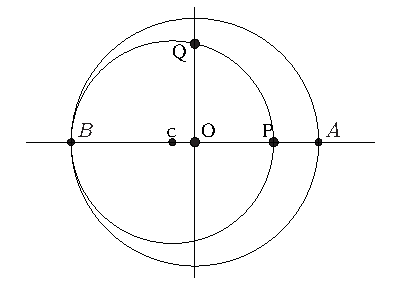
\includegraphics[width=0.5\textwidth]{pictures/squreroot.pdf}
\caption{squre root}
\end{figure}
If $A=(r,0)$ is constructible, so is $B=(-r, 0)$; $C$ is the midpoint of the segment $BP$ (midpoints are constructible); the circle with center $C$ and containing $P$ intersects the positive y-axis at a point $Q=(0,\delta)$, and elementary geometry shows that $\delta^2=r$. Therefore $\delta$ is constructible, concluding the proof of the theorem.
\end{proof}
\begin{corollary}\label{constructible number then degree power of 2}
Let $\gamma\in\mathscr{C}_{\C}$ be a constructible number. Then $[\Q(\gamma):\Q]$ is a power of $2$.
\end{corollary}
\begin{proof}
By Lemma~\ref{field constructible number} and Theorem~\ref{constructible number criterion}, there exist $\delta_1,\dots,\delta_k\in\R$ such that
\[\gamma\in\Q(\delta_1,\dots,\delta_k,i)\]
and each $\delta_j$ has degree $\leq 2$ over $\Q(\delta_1,\dots,\delta_{j-1})$. Repeated application of Proposition~\ref{field ext degree multiplicative} shows that
\[[\Q(\delta_1,\dots,\delta_k,i):\Q]\]
is a power of $2$, and since
\[\Q\sub\Q(\gamma)\sub\Q(\delta_1,\dots,\delta_k,i)\]
the claim follows from Corollary~\ref{field ext intermediate field degree divide}.
\end{proof}
As an example, constructing a regular $7$-gon would amount to constructing a $7$-th (complex) root of $1,\zeta$. By definition, $\zeta$ satisfies
\[t^7-1=(t-1)(t^6+t^5+\cdots+t+1)\]
as $\zeta\neq 1$, $\zeta$ must satisfy the cyclotomic polynomial $t^6+\cdots+1$. This is irreducible, hence again we find that $\zeta$ has degree $6$ over $\Q$, and Corollary~\ref{constructible number then degree power of 2} implies that the regular $7$-gon cannot be constructed with straightedge and compass.\par
Of course $7$ is not too special: if $p$ is a positive prime integer, the \textbf{cyclotomic polynomial} of degree $p-1$ is irreducible; hence
\[[\Q(\zeta_p):\Q]=p-1\]
where $\zeta_p$ is the complex $p$-th root of $1$ with argument $2\pi/p$. Therefore, Corollary~\ref{constructible number then degree power of 2} reveals that if $p$ is prime, then the regular $p$-gon can be constructed only if $p-1$ is a power of $2$. This is even more restrictive than it looks at first, due to the following simple lemma.
\begin{lemma}
If $2^k+1$ is prime, then $K$ is a power of $2$.
\end{lemma}
\begin{proof}
First note the fractorization:
\[t^{2m+1}+1=(t+1)(t^{2m}-t^{2m-1}+\cdots+1).\]
Thus $K$ is not odd. Assume that $k=2m$, then $2^k+1=2^{2m}+1=4^m+1$. Repeat this argument we see $m$ is also odd, and finally we conclude that $K$ is a power of $2$.
\end{proof}
Primes of the form $2^{2^\ell}+1$ are called \textbf{Fermat primes}. Therefore for a prime $p$, the regular $p$-gon if constructible only if $p$ is a Fermat prime.\par
We now use Galois theory to deal with the constructibility of regular $n$-gons. The key ingredient is the following result.
\begin{proposition}\label{prime power constr}
Let $E/K$ be a Galois extension, and assume $[F:K]=p^r$ for some prime $p$ and $r\geq 0$. Then there exist intermediate fields
\[K=E_0\sub E_1\sub E_2\sub\cdots\sub E_r=F\]
such that $[E_i:E_{i-1}]=p$ for $i=1,\dots,r$.
\end{proposition}
\begin{proof}
As the Galois correspondence is bijective for Galois extensions, this statement follows immediately from the fact that a group of order $p^r$, with $p$ prime, has a complete series of $p$-subgroups.
\end{proof}
\begin{theorem}\label{constructible regular n-gon iff}
The regular $n$-gon is constructible by straightedge and compass if and only if $\phi(n)$ is a power of $2$, if and only if $n=2^mp_1\cdots p_r$, where $m\geq 0$ and the factors $p_i$ are distinct Fermat primes.
\end{theorem}
\begin{proof}
We first prove the first equivalence. One direction is proved in Proposition~\ref{constructible number criterion}. For the converse, assume $\phi(n)=2^r$ for some $r$. The extension $\Q\sub\Q(\zeta_n)$ is Galois (it is the splitting field of $\Phi_n(X)$), of order $[\Q(\zeta_n):\Q]=\phi(n)=2^r$. Proposition~\ref{prime power constr} shows that the condition given in Theorem~\ref{constructible number criterion} is satisfied and therefore that $\zeta_n$ is constructible, as needed.\par
Now let $\phi(n)$ be a power of $2$. From the equation
\[\phi(n)=p_1^{k_1-1}(p_1-1)p_2^{k_2-1}(p_2-1)\cdots p_i^{k_i-1}(p_i-1)\]
we see that if $k_i-1>0$, then $p_i=2$. If $k_i-1=0$, then $p_i=2^m+1$ should be a prime, so $p_i$ is a Fermat prime. Hence $n=2^mp_1\cdots p_r$. The converse can also be deduced from the equality above.
\end{proof}
\subsection{The fundamental theorem of algebra}
\begin{theorem}
$\C$ is algebraically closed.
\end{theorem}
\begin{proof}
Let $f(X)\in\C[X]$ be a nonconstant polynomial; we have to prove that $f(X)$ has roots in $\C$. Note that if $f(X)$ has no roots in $\C$, then neither does $f(X)\widebar{f(X)}\in\R[X]$; that is, we may assume that $f(X)$ has real coefficients.\par
Now consider a tower $\R\sub\C\sub E$, where $E$ is a splitting field for $p(X)=(X^2+1)f(X)$ over $\R$. Since $[\C:\R]=2$ divides $[E:\R]$, we conclude that $[E:\R]=2^km$, for some $k>1$ with $m$ odd. Our goal is to show that $E=\C$, showing that $f(X)$ splits over $\C$.\par
Let $P$ be a $2$-Sylow subgroup of $\Gal_\R(f(X))$. Then $|P|=2^k$ and so
\[[E^P:\R]=[\Gal_\R(f(X)):P]=m.\]
By intermediate value theorem, every real polynomial with odd degree must have a root in $\R$, it follows that any nontrivial finite extension of $\R$ must have even degree (its primitive element must has even degree). From this we deduce that $m=1$ and $G=\Gal_\R(f(X))$ is a $2$-group of order $2^k$. Thus we have the tower
\[\{1\}\sub\Gal_\C(f(X))\sub G\]
in which $|\Gal_\C(f(X))|=2^{k-1}$. Therefore, according to Cauchy's theorem, $\Gal_\C(f(X))$ has a subgroup of any order dividing $2^{k-1}$. But $\Gal_\C(f(X))$ cannot have a subgroup of order $2^{k-2}$ that is, index $2$: if $H$ is such a group, then
\[\{1\}\sub H\sub\Gal_\C(f(X))\sub G\]
and then
\[2=[E^H:E^{\Gal_\C(f(X))}]=[E^H:\C],\]
which is impossible, since $\C$ does not have any irreducible polynomial of degree $2$. It follows that $|\Gal_\C(f(X))|=1$ and so $|G|=2$, which implies that $[E:\R]=2$, whence $E=\C$. 
\end{proof}
\subsection{Finite fields}
Let $F$ be a finite field, and let $p$ be its characteristic. We know that $F$ may be viewed as an extension
\[\F_p\sub F\]
of $\F_p=\Z/p\Z$; let $n=[F:F_p]$. Since $F$ has dimension $n$ as a vector space over $\F_p$, it is isomorphic to $\F_p^n$ as a vector space, and in particular $|F|=p^n$ is a power of $p$.
\subsubsection{Finite fields as splitting fields}
Let $F$ be a finite field of size $q$. Then $F^\times$ has order $q-1$ and so every element $\alpha\in F$ has exponent $q-1$, that is, $\alpha^{q-1}=1$. It follows that every element of $F$ is a root of the polynomial
\[f_q(X)=X^q-X\]
Since $f_q'(X)=-1$, this polynomial has no multiple roots and so $F$ is precisely the set of roots of $f_q(X)$ in some splitting field. In fact, since $F$ is a field, it is a splitting field for $f_q(X)$ over the prime subfield $\F_p$. We have the following theorem:
\begin{theorem}\label{finite field p^n order extension char}
Let $q=p^n$ be a power of a prime integer $p$.
\begin{itemize}
\item[(a)] The splitting field of the polynomial $f_q(X)=X^{q}-X$ over $\F_p$ is a field with precisely $q$ elements.
\item[(b)] Let $F$ be a field with exactly $q$ elements; then $F$ is a splitting field for $X^q-X$ over $\F_p$. The polynomial $X^q-X$ is separable over $\F_p$.
\end{itemize}
In particular, for every prime power $q$ there exists one and only one finite field of order $q$, up to isomorphism.
\end{theorem}
\begin{proof}
Let $F$ be the splitting field of $X^q-X$ over $\F_p$. Let $E$ be the set of roots of $f(X)=X^q-X$ in $F$. Since $f'(X)=qX^{q-1}-1=-1$ (as $q=0$ in characteristic $p$), we have $(f(X),f'(X))=1$; hence by Proposition~\ref{poloynomial separable iff f'} $f(X)$ is separable, and $E$ consists of precisely $q$ elements. We claim that $E$ is a field, and it follows that $E=F$.\par
To see that $E$ is a field, let $a,b\in E$. Then $a^q=a$ and $b^q=b$; it follows that
\[(a-b)^q=a^p+(-1)^qb^q=a^q-b^q=a-b.\]
(note that $(-1)^q=-1$ if $p$ is odd and $(-1)^q=+1=-1$ if $p=2$). If $b\neq0$,
\[(ab^{-1})^q=a^q(b^q)^{-1}=ab^{-1}.\]
Thus $E$ is closed under subtraction and division by a nonzero element, proving that $E$ is a field and concluding the proof of the first statement.\par
To prove the second statement, let $F$ be a field with exactly $q$ elements. The nonzero elements of $F$ form a group under multiplication consisting of $q-1$ elements. Therefore for any elments in $a\in F^\times$ we have $a^{q-1}=1$. Of course $0^q-0=0$, so the polynomial $X^q-X$ has $q$ roots in $F$; it follows that $F$ is a splitting field for $X^q-X$, as stated. The final statement comes from the uniqueness of splitting fields. This completes the proof.
\end{proof}
Let us refer to the polynomial $f_q(X)=X^q-X$ as the \textbf{defining polynomial} of the finite field $\F_{p^n}$. In view of this theorem, we will often refer to the finite field $\F_{p^n}$.\par
An immediate consequence of the splitting field characterization of finite fields is that any extension of finite fields is normal.
\begin{corollary}
The extension $\F_{p}\sub\F_{p^n}$ is a finite Galois extension. Hence, in the Galois correspondence for $\F_p\sub\F_{p^n}$, all intermediate fields and all subgroups are closed.
\end{corollary}
\begin{example}
Let $p$ be a prime integer. Then we claim that the polynomial $X^4+1$ is \textbf{reducible} over $\F_p$ (and therefore over every finite field).\par
Since $X^4+1=(X+1)^4$ in $\F_2[X]$, the statement holds for $p=2$. Thus, we may assume that $p$ is an odd prime. Then we claim that $X^4+1$ divides $X^{p^2}-X$. Indeed, the square of every odd number is congruent to $1$ mod $8$; hence $X^8-1$ divides $X^{p^2-1}-1$, which implies
\[(X^4+1)\mid(X^8-1)\mid(X^{p^2-1}-1)\mid(X^{p^2}-X)\]
It follows that $X^4+1$ factors completely in the splitting field of $X^{p^2}-X$, that is, in $\F_{p^2}$. If $\alpha$ is a root of $X^4+1$ in $\F_{p^2}$, we have the extensions
\[\F_p\sub \F_p(\alpha)\sub\F_{p^2}\]
therefore $[\F_p(\alpha):\F_p]$ divides $[\F_{p^2}:\F_p]=2$. That is, $\alpha$ has degree $1$ or $2$ over $\F_p$. But then its minimal polynomial is a factor of degree $1$ or $2$ of $(X^4+1)$,
showing that the latter is reducible.
\end{example}
Now we wish to examine the subfields of a finite field $\F_{p^n}$. Note that if $d$ and $n$ are positive integers and $n=kd+r$ for $0\leq r<d$, then it is easy to see $X^d-1\mid X^n-1$ if and only if $d\mid n$. This yields the following result on subfields of $\F_{p^n}$.
\begin{proposition}[\textbf{Classfication of Subfields of $\F_{p^n}$}]\label{finite field subfield iff order divide}
The following are equivalent:
\begin{itemize}
\item[(\rmnum{1})] The interger $d$ divides $n$.
\item[(\rmnum{2})] The defining polynomial $f_{p^d}(X)$ divides the defining polynomial $f_{p^n}(X)$.
\item[(\rmnum{3})] The field $\F_{p^d}$ is contained in $\F_{p^n}$. 
\end{itemize}
Put another way, the following lattices are isomorphic:
\begin{itemize}
\item[(a)] $\{d:\text{$d$ divides $n$}\}$, under division.
\item[(b)] $\{f_{p^d}(X):\text{$f_{p^d}(X)$ divides $f_{p^n}(X)$}\}$, under division.
\item[(c)] Subfields of $\F_{p^n}$, under set inclusion.
\end{itemize}
Moreover, $\F_{p^n}$ has exactly one subfield of size $p^d$, for each $d$ divides $n$, and each extension $\F_{p^d}\sub\F_{p^n}$ is simple.
\end{proposition}
\begin{proof}
To start with, we first prove the following facts:
\begin{align}\label{finite field subfield iff order divide-1}
p^d-1\mid p^n-1\Leftrightarrow d\mid n\Leftrightarrow X^d-1\mid X^n-1
\end{align}
In fact, write $n=kd+r$ with $0\leq r<d$, then
\[X^{n}-1=X^{kd+r}-X^r+X^r-1=X^r(X^{kd}-1)+X^r-1.\]
Since $X^d-1\mid X^{kd}-1$, this implies
\[X^n-1\equiv X^r-1\quad \text{mod $X^d-1$}\]
which proves (\ref{finite field subfield iff order divide-1}) immediately. Now apply these results with Proposition~\ref{finite field p^n order extension char}, we obtain that
\[d\mid n\Leftrightarrow p^d-1\mid p^n-1\Leftrightarrow X^{p^d-1}-1\mid X^{p^n-1}-1\Leftrightarrow f_{p^d}(X)\mid f_{p^n}(X).\]
which says (\rmnum{1}) and (\rmnum{2}) are equivalent. Moreover, by Proposition~\ref{finite field p^n order extension char},
\[\F_{p^d}\sub\F_{p^n}\Leftrightarrow\text{Root}(f_{p^d}(X))\sub\text{Root}(f_{p^n}(X))\Leftrightarrow f_{p^d}(X)\mid f_{p^n}(X).\]
so (\rmnum{2}) and (\rmnum{3}) are also equivalent. Moreover, if $\F_{p^n}$ has two distinct subfields of size $p^d$, then the polynomial $f_{p^d}(X)$ would have more than $p^d$ roots in $\F_{p^n}$, which is impossible.\par
For the last statement, recall that the multiplicative group of nonzero elements of a finite field is cyclic. If $\alpha\in\F_{p^n}$ is a generator of this gorup, then $\alpha$ will generate $\F_{p^n}$ over any subfield. If $d\mid n$, then $\F_{p^n}=\F_{p^d}(\alpha)$, so this extension is simple.
\end{proof}
These results can be translated into rather precise information on the structure of the polynomial ring over a finite field. For example,
\begin{corollary}\label{finite field irre poly of any order}
Let $F$ be a finite field. Then for all integers $n\geq1$ there exist irreducible polynomials of degree $n$ in $F[X]$.
\end{corollary}
\begin{proof}
We know $F=\F_{q}$ for some prime power $q$. By Corollary~\ref{finite field subfield iff order divide} there is an extension $\F_{q}\sub\F_{q^{n}}$, generated by an element $\alpha$. Then $[F_{q^{n}}:\F_{q}]=n$, and it follows that the minimal polynomial of $\alpha$ over $F=\F_{q}$ is an irreducible polynomial of degree $n$ in $F[X]$.
\end{proof}
In fact, our analysis of extensions of finite fields tells us about explicit factorizations, leading to an inductive algorithm for the computation of irreducible polynomials in $\F_q[X]$:
\begin{corollary}
Let $F=\F_q$ be a finite field, and let $n$ be a positive integer. Then the factorization of $X^{q^n}-X$ in $F[X]$ consists of all irreducible monic polynomials of degree $d$, as $d$ ranges over the positive divisors of $n$. In particular, all these polynomials factor completely in $\F_{q^n}$, and each irreducible polynomial appears only once in the factorization.
\end{corollary}
\begin{proof}
By Theorem~\ref{finite field p^n order extension char}, $\F_{q^n}$ is the splitting field of $X^{q^n}-X$ over $\F_p$, and hence over $\F_q=F$.\par
If $f(X)$ is a monic irreducible polynomial of degree $d$, then $F[X]/(f(X))=F(\alpha)$ is an extension of degree $d$ of $F$, that is, an isomorphic copy of $\F_{q^d}$. By Corollary~\ref{finite field subfield iff order divide}, if $d\mid n$, then there is an embedding of $\F_{q^d}$ in $\F_{q^n}$. But then $\alpha$ must be a root of $X^{q^n}-X$, and hence $X^{q^n}-X$ is a multiple of $f(X)$, as this is the minimal polynomial of $\alpha$. This proves that every irreducible polynomial of degree $d\mid n$ is a factor of $X^{q^n}-X$.\par
Conversely, if $f(X)$ is an irreducible factor of $X^{q^n}-X$, then $\F_{q^n}$ contains a root $\alpha$ of $f(X)$; we have the extensions $F=\F_q\sub\F_q(\alpha)\sub\F_{q^n}$, and $\F_q(\alpha)\cong\F_{q^d}$ for $d=\deg\alpha$. It follows that $d\mid n$, again by Corollary~\ref{finite field subfield iff order divide}.\par
For the last statement, note that $(X^{p^n}-X)'=p^nX^{p^n-1}-1=-1$, so $X^{p^n}-X$ is separable by Proposition~\ref{poloynomial separable iff f'}. This implies each irreducible polynomial appears only once in $X^{p^n}-X$.
\end{proof}
The picture we are trying to convey is the following: the $q^n$ roots of $X^{q^n}-X$ clump into disjoint subsets, with each subset collecting the roots of each and every irreducible polynomial of degree $d\mid n$ in $F[X]$.
\begin{example}
Let's contemplate the case $q=2$: $\F_2=\Z/2\Z$.
\begin{itemize}
\item $n=1$: the polynomial $X^2-X$ factors as the product of $X$ and $(X-1)$ (which we could write as $(X+1)$ just as well, since we are working over $\F_2$). These are all the irreducible polynomials of degree $1$ over $\F_2$.
\item $n=2$: the polynomial $X^4-X$ must factor as the product of all irreducible polynomials of degree $1$ and $2$; in fact
\[X^4-X=X(X-1)(X^2+X+1)\]
and the conclusion is that there is exactly one irreducible polynomial of degree $2$ over $\F_2$, namely $X^2+X+1$.
\item $n=3$: the quotient of $X^8-X$ by $X(X-1)$ is a polynomial of degree $6$, which must therefore be the product of the two irreducible polynomials of degree $3$ over $\F_2$. It takes a moment to find them:
\[X^3+X^2+1,\quad X^3+X+1\]
It also follows that $\F_8$ may be realized in two ways as a quotient of $\F_2[X]$ modulo an irreducible polynomial:
\[\dfrac{\F_2[X]}{(X^3+X^2+1)}\cong\dfrac{\F_2[X]}{(X^3+X+1)}\]
\end{itemize}
\end{example}
Since extensions of finite fields are simple extensions, our previous work allows us to be much more precise. Restricting our attention to the extensions $\F_p\sub\F_{p^n}$, for a prime $p$, we know these can be realized as simple extensions by an element with minimal polynomial of degree $n$. This polynomial is necessarily separable ($\F_p$ is perfect), so Corollary~\ref{field simple ext order of Aut} immediately gives us the size of the automorphism group: $|\Gal(\F_{p^n}/\F_p)|=n$.
\begin{proposition}\label{finite field Galois generated by Frobenius}
The Galois group $G$ of $\F_{p^n}$ over $\F_p$ is cyclic of order $n$, generated by the Frobenius automorphism.
\end{proposition}
\begin{proof}
We have seen that the Frobenius isomorphism $\sigma$ is an automorphism of $\F_{p^n}$. If $\alpha\in\F_{p}$, then $\sigma(\alpha)=\alpha^p=\alpha$ and so $\sigma$ fixes $\F_{p}$ and is therefore in the Galois group $G$. Moreover, the $n$ automorphisms
\[1,\sigma,\sigma^2,\dots,\sigma^{n-1}\]
are distinct elements of $G$, for if $\sigma^k=1$ then $\alpha^{p^k}=\alpha$ for all $\alpha\in\F_{p^n}$ and so $\F_{p^n}\sub\F_{p^d}$, which implies that $k\geq n$. Finally, since $|G|=n$, we see that $G=\langle\sigma\rangle$.
\end{proof}
\begin{corollary}\label{finite field F_pn over F_pd char}
Let $d\mid n$ be positive integers, then the Galois group $G$ of $\F_{p^n}$ over $\F_{p^d}$ is cyclic of order $n/d$, generated by the automorphism $\sigma^d:\alpha\mapsto\alpha^{p^d}$.
\end{corollary}
\begin{proof}
Let $\sigma^d$ be the automorphism prescribed above. Then $\sigma^d$ fixes $\F_{p^d}$.and hence is in $G$, and it has order $d/n$. By Theorem~\ref{Galois fundamental theorem-3} we have
\[\Gal(\F_{p^d}/\F_p)\cong\frac{\Gal(\F_{p^n}/\F_p)}{\Gal(\F_{p^n}/\F_{p^d})},\]
and in particular $|\Gal(\F_{p^n}/\F_{p^d})|=n/d$. Since $\sigma^{d}$ also has order $n/d$, the claim follows.
\end{proof}
\begin{corollary}\label{finite field F_p absolute Galois group char}
The absolute Galois group $\Gal(\widebar{\F}_p/\F_p)$ is isomomorphic to $\widehat{\Z}=\llim\Z/n\Z$.
\end{corollary}
\begin{proof}
Let $F=\F_q$ be a finite field. We show that the absolute Galois group is isomomorphic to $\widehat{\Z}$. For this, let $\mathcal{N}$ be the category associated to the poset $\N$ of division partial order, and we still denote by $n$ the objects of $\mathcal{N}$. By Proposition~\ref{finite field subfield iff order divide} we have an inverse system of groups
\[\big(\Gal(\F_{q^n}/\F_q)\big)_{n\in\mathcal{N}}\]
where for $m\mid n$ the map $\Gal(\F_{q^n}/\F_q)\to\Gal(\F_{q^m}/\F_q)$ is the restriction map; that is, the image of an automorphism $\sigma\in\Gal(\F_{q^n}/\F_q)$ in $\Gal(\F_{q^m}/\F_q)$ is obtained by simply restricting the domain of $\sigma$ from $\F_{q^n}$ to $\F_{q^m}$. Since $\F_{q^m}$ are all the finite subextensions of $\widebar{\F}_q$, by Corollary~\ref{Galois group identified as inverse limit}, we see the inverse limit of this inverse system is exactly $\Gal(\widebar{F}_q/\F_q)$. But Corollary~\ref{finite field F_pn over F_pd char} suggests that $\Gal(\F_{q^n}/\F_q)\cong\Z/n\Z$ and the restriction map corresponds to the quotient map $\Z/n\Z\to Z/m\Z$. Thus the inverse system $\big(\Gal(\F_{q^n}/\F_q)\big)_{n\in\mathcal{N}}$ is isomorphic to $(\Z/n\Z)_{n\in\mathcal{N}}$ and the claim follows from this.
\end{proof}
\subsubsection{The algebraic closure of a finite field}
To conclude, we determine the algebraic closure of a finite field $\F_{p}$. Since $\F_{p}\sub\F_{p^n}$ is algebraic for all positive integers $n$, an algebraic closure of $\F_p$ must contain all of the fields $\F_{p^n}$. Since $n!\mid(n+1)!$, it follows that $\F_{p^{n!}}\sub\F_{p^{(n+1)!}}$ and so the union
\[\Gamma(p)=\bigcup_{n=0}^{\infty}\F_{p^{n!}}\]
is an extension field of $\F_p$ that contains $\F_{p^n}$ for all $n\geq 1$. Moreover, if $E$ is a field for which $\F_{p^n}\sub E$ for all $n$, then $\Gamma(p)\sub E$, that is, $\Gamma(p)$ is the smallest field containing each $\F_{p^n}$.
\begin{theorem}
The field $\Gamma(p)$ is the algebraic closure of $\F_p$.
\end{theorem}
\begin{proof}
Every element of $\Gamma(p)$ lies in some $\F_{p^{n!}}$, whence it is algebraic over $\F_p$. Thus $\Gamma(p)$ is algebraic over $\F_p$. Now let $f(X)$ be an irreducible polynomial over $\Gamma(p)$ of degree $d$. Then the coefficients of $f(X)$ lie in some $\F_{p^{n!}}$ and so $f(X)$ is irreducible as a polynomial over $\F_{p^{n!}}$. Hence, the splitting field for $f(X)$ is $\F_{p^{n!d}}\sub\Gamma(p)$ and so $\Gamma(p)$ splits over $\Gamma(p)$.
\end{proof}
\subsection{Cyclotomic polynomials and fields}
Let $K$ be a field. By a \textbf{root of unity} (in $K$) we shall mean an element $\zeta\in K$ such that $\zeta^n=1$ for some integer $n>1$. If the characteristic of $K$ is $p$, then the equation
\[X^{p^d}=1\]
has only one root, namely $1$, and hence there is no $p^d$-th root of unity except $1$.\par
Let $n$ be an integer $>1$ and not divisible by the characteristic $p$. The polynomial
\[X^n-1\]
is separable because its derivative is $nX^{n-1}\neq 0$, and the only root of the derivative is $0$, so there is no common root. Hence in $\widebar{K}$ the polynomial $X^n-1$ has $n$ distinct roots, which are roots of unity. They obviously form a group, and we know that every finite multiplicative group in a field is cyclic. Thus the group of $n$-th roots of unity is cyclic. A generator for this group is called a \textbf{primitive $\bm{n}$-th root} of unity.\par
If $\mu_n$ denotes the group of all $n$-th roots of unity in $\widebar{n}$ and $m,n$ are relatively prime integers, then
\[\mu_{mn}\cong\mu_m\times\mu_n\]
This follows because $\mu_m$, $\mu_n$ cann ot have any element in common except $1$, and because $\mu_m\mu_n$ consequently has $mn$ elements, each of which is an $mn$-th root of unity. Hence $\mu_m\mu_n=\mu_{mn}$ and the decomposition is that of a direct product.\par
As a matter of notation, to avoid double indices, especially in the prime power case, we write $\mu[n]$ for $\mu_n$. So if $p$ is a prime, $\mu[p^r]$ is the group of $p^r$-th roots of unity. Then $\mu[p^{\infty}]$ denotes the union of all $\mu[p^r]$ for all positive integers $r$.\par
Let $K$ be any field. Let $n$ be not divisible by the characteristic $p$. Let $\zeta_n$ be a primitive $n$-th root of unity in $\widebar{K}$. Let $\sigma$ be an embedding of $K(\zeta)$ in $\widebar{K}$ over $K$. Then
\[(\sigma(\zeta))^n=\sigma(\zeta^n)=1\]
so that $\sigma(\zeta)$ is an $n$-th root of unity also. Hence $\sigma(\zeta)=\zeta^i$ for some integer $i=i(\sigma)$, uniquely determined mod $n$. It follows that $\sigma$ maps $K(\zeta)$ into itself, and hence that $K(\zeta)$ is normal over $K$. If $\tau$ is another automorphism of $K(\zeta)$ over $K$ then
\[\sigma(\tau(\zeta))=\zeta^{i(\sigma)i(\tau)}\]
Since $\sigma$ and $\tau$ are automorphisms, it follows that $i(\sigma)$ and $i(\tau)$ are coprime to $n$. In this way we get a homomorphism of the Galois group $G$ of $K(\zeta)$ over $K$ into the multiplicative group $(\Z/n\Z)^\times$ of integers prime to $n$, mod $n$. Our homomorphism is clearly injective since $i(\sigma)$ is uniquely determined by $\sigma$ mod $n$, and the effect of $\sigma$ on $K(\zeta)$ is determined by its effect on $\zeta$. We conclude that $K(\zeta)$ is abelian over $K$. We know that the order of $(\Z/n\Z)^\times$ is $\phi(n)$. Hence the degree
$[K(\zeta):K]$ divides $\phi(n)$.\par
For a specific field $K$, the question arises whether the image of $\Gal(K(\zeta)/K)$ in $(\Z/n\Z)^\times$ is all of $(\Z/n\Z)^\times$. Looking at $K=\R$ or $\C$, one sees that this is not always the case. We now give an important example when it is the case.\par
Define the $n$-th \textbf{cyclotomic polynomial} $\Phi_n(X)$ to be
\[\Phi_n(X)=\prod_{\zeta\text{ primitive $n$-th root of }1}(X-\zeta)=\prod_{\substack{1\leq m\leq n\\(m,n)=1}}(X-\zeta_n^m)\]
which has degree $\phi(n)$.
\begin{example}
If $n=p$ is prime, then every nonidentity element of $\mu_p\cong C_p$ is a generator: every $p$-th root of $1$ is primitive except $1$ itself. Therefore
\[\Phi_p(X)=\dfrac{X^p-1}{X-1}=X^{p-1}+\cdots+X+1\]
\end{example}
\begin{lemma}\label{cyclotomic polynomial lemma}
For all positive integers $n$,
\[X^n-1=\prod_{\substack{1\leq d\leq n\\d\mid n}}\Phi_d(X)\]
\end{lemma}
\begin{proof}
If $n=de$, then every $d$-th root $\zeta$ of $1$ is an $n$-th root of $1$, because $\zeta^n=\zeta^{de}=(\zeta^d)^e=1$. In particular, every primitive $d$-th root $\zeta$ of $1$ is an $n$-th root of $1$.\par
On the other hand, every $\zeta\in \mu_n$ generates a subgroup $H$ of $\mu_n$, and $H=\mu_d$ for
$d$ equal to the order of $\zeta$, a divisor of $n$. Thus, every $\zeta\in \mu_n$ is a primitive $d$-th root of $1$ for some $d\mid n$.\par
Thus the set of $n$-th roots of $1$ equals the union of the sets of primitive $d$-th roots of $1$, as $d$ ranges over all positive divisors of $n$. The statement follows immediately:
\[X^n-1=\prod_{\zeta\in \mu_n}(X-\zeta)=\prod_{\substack{1\leq d\leq n\\d\mid n}}\Bigg(\prod_{\zeta\text{ primitive $d$-th root of }1}(X-\zeta)\Bigg)=\prod_{\substack{1\leq d\leq n\\d\mid n}}\Phi_d(X)\]
as claimed.
\end{proof}
Lemma~\ref{cyclotomic polynomial lemma} yields an inductive computation of cyclotomic polynomials; the fact that $\Phi_n(X)\in\Z[X]$ follows from this fact. Explicitly,
\begin{corollary}
The cyclotomic polynomials $\Phi_n(X)$ have integer coefficients.
\end{corollary}
\begin{proof}
Use induction on $n$. Note that $\Phi_1(X)=x-1$, and assume we have shown that all $\Phi_m(X)$ have integer coefficients for $m<n$. In particular, $f(X):=\prod_{1\leq d\mid n,d<n}\Phi_d(X)$ is a monic polynomial with integer coefficients. Since $f(X)$ is monic, we can divide it into $X^n-1$ with remainder, within $\Z[X]$: there exist $q(X),r(X)\in\Z[X]$ such that
\[X^n-1=q(X)f(X)+r(X)\]
with $r(X)=0$ or $\deg r(X)<\deg f(X)$. On the other hand, by Lemma~\ref{cyclotomic polynomial lemma},
\[X^n-1=f(X)\Phi_n(X)\]
in $\C[X]$. Therefore
\[f(X)(\Phi_n(X)-q(X))=r(X)\]
in $\C[X]$. But this forces $r(X)=0$ (otherwise we would have $\deg r(X)>\deg f(X)$). Therefore $\Phi_n(X)=q(X)\in\Z[X]$.
\end{proof}
\begin{proposition}
For all positive $n$, $\Phi_n(X)\in\Z[X]$ is irreducible over $\Q$.
\end{proposition}
\begin{proof}
Arguing by contradiction, assume $\Phi_n(X)$ is reducible. Then its roots $\zeta_n^m$, with $(m,n)=1$, are divided among the factors; we can choose a root $\zeta^m_n$ of one irreducible monic factor $f(X)$, such that another root $\zeta^{mp}_n$ (for some prime $p$ not dividing $n$) is not a root of $f(X)$. Write 
\[\Phi_n(X)=f(X)g(X)\]
since $\Phi_n(X)\in\Z[X]$ and $\Phi_n(X)$, $f(X)$ are monic, $f(X)$ and $g(X)$ have integer coefficients. By our choice, $f(X)$ is the minimal polynomial of $\zeta^m_n$ over $\Q$, and $g(\zeta^{mp}_n)=0$.\par
It follows that $\zeta^m_n$ is a root of $g(X^p)$, and hence $f(X)\mid g(X^p)$. Therefore we can
write
\[g(X^p)=f(X)h(X)\]
with $h(X)\in\Z[X]$. Reading the last equation modulo $p$, we get (again using $(a+b)^p=a^p+b^p$, and denoting cosets by bar)
\[\widebar{g}(X)^p=\widebar{f}(X)\widebar{h}(X)\text{in }\F_p[X].\]
In particular, $\widebar{f}(X)$ and $\widebar{g}(X)$ must have a nontrivial common factor $\widebar{\ell}(X)$ in $\F_p[X]$. But then
\[\ell^2(X)\mid\widebar{f}(X)\widebar{g}(X)\]
the reduction of $\Phi_n(X)$ modulo $p$ must have a multiple factor.\par
This implies that $X^n-1\in\F_p[X]$ has a multiple factor; that is, it is inseparable. However, its derivative $nX^{n-1}\in\F_p[X]$ is nonzero (because $p$ does not divide $n$ by assumption), and Proposition~\ref{poloynomial separable iff f'} implies that $X^n-1$ is separable in $\F_p[X]$.\par
This contradiction shows that our assumption that $\Phi_n(X)$ is reducible must be nonsense, proving the statement.
\end{proof}
\begin{definition}
The splitting field $\Q(\zeta_n)$ for the polynomial $X^n-1$ over $\Q$ is the $n$-th \textbf{cyclotomic field}.
\end{definition}
\begin{proposition}\label{Galois group of cyclotomic field}
The Galois group $\Gal(\Q(\zeta_n)/\Q)$ is isomorphic to $(\Z/n\Z)^\times$.
\end{proposition}
\begin{proof}
We know that $\Gal(\Q(\zeta_n)/\Q)$ has cardinality $\phi(n)$ (Corollary~\ref{field simple ext order of Aut}; the roots
are distinct since $\Phi_n(X)$ is separable), so the homomorphism $\Gal(\Q(\zeta_n)/\Q)\to(\Z/n\Z)^\times$ is an isomorphism.
\end{proof}
\begin{corollary}
If $n,m$ are relative prime integers, then
\[\Q(\zeta_m)\cap\Q(\zeta_n)=\Q.\]
\end{corollary}
\begin{proof}
We note that $\zeta_n$ and $\zeta_m$ are both contained in $\Q(\zeta_{mn})$ since $\zeta_{mn}^n$ is a primitive $m$-th root of unity. Furthermore, $\zeta_{m}\zeta_n$ is a primitive $mn$-th root of unity. Hence
\[\Q(\zeta_m)\Q(\zeta_n)=\Q(\zeta_{mn})\]
Our assertion then follows from the multiplicativity $\phi(mn)=\phi(m)\phi(n)$ and Proposition~\ref{Galois group of lifting}.
\end{proof}
\begin{example}
The reader should consider Examples~\ref{split field of x^8-1} again: by what we have just proved, the automorphism group of the splitting field of $X^8-1$ is isomorphic to the group of units in $\Z/8\Z$; this group is immediately seen to be isomorphic to $(\Z/2\Z)\times(\Z/2\Z)$, confirming the claim made in Example~\ref{split field of x^8-1}.
\end{example}
\subsection{Cyclic extensions}
\subsubsection{Hilbert's theorem 90}
Let $G$ be a group. A \textbf{$\bm{G}$-module} is an abelian group $M$ together with an action of $G$, i.e., a map $G\times M\to M$ such that
\begin{itemize}
\item $\sigma(m+n)=\sigma m+\sigma n$ for $m,n\in M$.
\item $(\sigma\tau)m=\sigma(\tau m)$ for $\sigma,\tau\in G$ and $m\in M$.
\item $1m=m$ for $m\in M$.
\end{itemize}
Thus, to give an action of $G$ on $M$ is the same as giving a homomorphism $G\to\Aut(M)$ (automorphisms of $M$ as an abelian group).
\begin{example}
Let $E$ be a Galois extension of $K$ with Galois group $G$. Then $(E,+)$ and $(E^\times,\times)$ are $G$-modules.
\end{example}
Let $M$ be a $G$-module. A \textbf{crossed homomorphism} is a map $f:G\to  M$ such that
\[f(\sigma\tau)=f(\sigma)+\sigma f(\tau)\]
for all $\sigma,\tau\in G$. Note that the condition implies that $f(1)=f(1)+f(1)$, and so $f(1)=0$.
\begin{example}
\mbox{}
\begin{itemize}
\item[$(a)$] Let $f:G\to M$ be a crossed homomorphism. For any $g\in G$,
\begin{equation*}
\begin{aligned}
f(\sigma^2)&=f(\sigma)+\sigma f(\sigma),\\
f(\sigma^3)&=f(\sigma)+\sigma f(\sigma^2)=f(\sigma)+\sigma f(\sigma)+\sigma^2 f(\sigma)\\
&\ \ \vdots\\
f(\sigma^n)&=f(\sigma)+\sigma f(\sigma)+\cdots+\sigma^{n-1}f(\sigma)
\end{aligned}
\end{equation*}
Thus, if $G$ is a cyclic group of order $n$ generated by $\sigma$, then a crossed homomorphism $f:G\to M$ is determined by its value, $x$ say, on $\sigma$, and $x$ satisfies the equation
\begin{align}\label{cross homomorphism cyclic}
x+\sigma x+\cdots+\sigma^{n-1}x=0
\end{align}
Moreover, if $x\in M$ satisfies $(\ref{cross homomorphism cyclic})$, then the formulas $f(\sigma^i)=x+\sigma x+\cdots+\sigma^{i-1}x$ define a crossed homomorphism $f:G\to M$. Thus, for a finite cyclic group $G=\langle\sigma\rangle$, there is a one-to-one correspondence
\[\{\text{crossed homomorphisms $f:G\to M$}\}\leftrightarrows\{\text{$x\in M$ satisfying $(\ref{cross homomorphism cyclic})$}\}.\]
\item[$(b)$] For every $x\in M$, we obtain a crossed homomorphism by putting
\[f(\sigma)=\sigma x-x\] 
for all $\sigma\in G$. A crossed homomorphism of this form is called a \textbf{principal crossed homomorphism}.
\item[$(c)$] If $G$ acts trivially on $M$, i.e., $\sigma m=m$ for all $\sigma\in G$ and $m\in M$, then a crossed homomorphism is simply a homomorphism, and there are no nonzero principal crossed homomorphisms.
\end{itemize}
\end{example}
The sum and difference of two crossed homomorphisms is again a crossed homomorphism, and the sum and difference of two principal crossed homomorphisms is again principal. Thus we can define
\[H^1(G,M)=\frac{\text{crossed homomorphisms}}{\text{principal crossed homomorphisms}}\]
(quotient abelian group). An exact sequence of $G$-modules
\[\begin{tikzcd}
0\ar[r]&M\ar[r]&N\ar[r]&L\ar[r]&0
\end{tikzcd}\]
gives rise to an exact sequence
\[\begin{tikzcd}[column sep=scriptsize]
0\ar[r]&M^G\ar[r]&N^G\ar[r]&L^G\ar[r,"\delta"]&H^1(G,M)\ar[r]&H^1(G,N)\ar[r]&H^1(G,L)
\end{tikzcd}\]
Let $\ell\in L^G$, and let $n\in N$ map to $\ell$. For all $\sigma\in G$, $\sigma n-n$ lies in the submodule $M$ of $N$, and the crossed homomorphism $\sigma\mapsto\sigma n-n:G\to M$ represents $\delta(\ell)$.
\begin{example}
Let $\pi:\widetilde{X}\to X$ be the universal covering space of a topological space $X$, and let $\Gamma$ be the group of covering transformations. Under some fairly general hypotheses, a $\Gamma$-module $M$ will define a sheaf $\mathcal{M}$ on $X$, and $H^1(X,\mathcal{M})\cong H^1(\Gamma,M)$. For example, when $M=\Z$ with the trivial action of $\Gamma$, this becomes the isomorphism $H^1(X,\Z)\cong H^1(\Gamma,\Z)=\Hom(\Gamma,\Z)$.
\end{example}
\begin{theorem}\label{field ext H^1(G,E^*) H^1(G,E) is trivial}
Let $E$ be a finite Galois extension of $K$ with group $G$; then $H^1(G,E^{\times})=0$ and $H^1(G,E)=0$.
\end{theorem}
\begin{proof}
Let $f$ be a crossed homomorphism $G\to E^\times$. In multiplicative notation, this means that
\[f(\sigma\tau)=f(\sigma)\cdot (\sigma f(\tau))\]
for $\sigma,\tau\in G$, and we have to find a $\gamma\in E^\times$ such that $f(\sigma)=\sigma(\gamma)/\gamma$ for all $\sigma\in G$. Because the $f(\tau)$ are nonzero, Corollary~\ref{field embedding independent} implies that
\[\sum_{\tau\in G}f(\tau)\tau:E\to E\]
is not the zero map, i.e., there exists an $\alpha\in E$ such that
\[\beta:=\sum_{\tau\in G}f(\tau)\tau(\alpha)\neq 0.\]
But then, for $\sigma\in G$,
\begin{align*}
\sigma(\beta)&=\sigma\Big(\sum_{\tau\in G}f(\tau)\tau(\alpha)\Big)=\sum_{\tau\in G}\sigma(f(\tau))\sigma(\tau(\alpha))\\
&=f(\sigma)^{-1}\sum_{\tau\in G}f(\sigma\tau)(\sigma\tau)(\alpha)=f(\sigma)^{-1}\beta.
\end{align*}
Therefore $f(\sigma)=\beta/\sigma(\beta)$ and we can take $\gamma=\beta^{-1}$.\par
For the additive version, let $f:G\to E$ be a crossed homomorphism. Then we have
\[f(\sigma\tau)=f(\sigma)+\sigma f(\tau)\]
for $\sigma,\tau\in G$. Let $\gamma\in E$ an element in $E$ such that $\tr(\gamma)\neq 0$ (this element exists by linearly independence), and consider
\[\beta:=\sum_{\tau\in G}f(\tau)\tau(\gamma).\]
Then we have
\begin{align*}
\sigma(\beta)&=\sigma\Big(\sum_{\tau\in G}f(\tau)\tau(\gamma)\Big)=\sum_{\tau\in G}\sigma(f(\tau))\sigma(\tau(\gamma))\\
&=\sum_{\tau\in G}f(\sigma\tau)(\sigma\tau)(\gamma)-f(\sigma)\sum_{\tau\in G}(\sigma\tau)(\gamma)=\beta-f(\sigma)\tr(\gamma).
\end{align*}
Since $\tr(\gamma)\neq 0$, we obtain $f(\sigma)=\beta/\tr(\gamma)-\sigma(\beta/\tr(\gamma))$, so $f$ is principal.
\end{proof}
\begin{corollary}[\textbf{Hilbert's theorem 90, multiplicative version}]
Let $E$ be a finite cyclic extension of $K$ and let $\sigma$ generate $\Gal(E/K)$. Let $\alpha\in E$, if $N(\alpha)=1$, then $\alpha=\beta/\sigma(\beta)$ for some $\beta\in E$.
\end{corollary}
\begin{proof}
Let $n=[E:K]$. The condition on $\alpha$ is that $\alpha\sigma(\alpha)\cdots\sigma^{n-1}(\alpha)=1$, and so by $(\ref{cross homomorphism cyclic})$ there is a crossed homomorphism $f:G\to E^{\times}$ with $f(\sigma)=\alpha$. Theorem~\ref{field ext H^1(G,E^*) H^1(G,E) is trivial} now shows that $f$ is principal, which means that there is a $\beta\in E$ such that $\alpha=\beta/\sigma(\beta)$.
\end{proof}
\begin{corollary}[\textbf{Hilbert's theorem 90, additive version}]
Let $E$ be a finite cyclic extension of $K$ and let $\sigma$ generate $\Gal(E/K)$. Let $\alpha\in E$, if $\tr(\alpha)=0$, then $\alpha=\beta-\sigma(\beta)$ for some $\beta\in E$.
\end{corollary}
\begin{proof}
Let $n=[E:K]$. The condition on $\alpha$ is that $\alpha+\sigma(\alpha)+\cdots+\sigma^{n-1}(\alpha)=1$, and so by $(\ref{cross homomorphism cyclic})$ there is a crossed homomorphism $f:G\to E$ with $f(\sigma)=\alpha$. Theorem~\ref{field ext H^1(G,E^*) H^1(G,E) is trivial} now shows that $f$ is principal, which means that there is a $\beta\in E$ such that $\alpha=\beta/\sigma(\beta)$.
\end{proof}
\subsubsection{Abelian and Cyclic Extensions}
Extensions are often named after their Galois groups. Here is a very important example.
\begin{definition}
A Galois extension $E/K$ is \textbf{abelian} if its Galois group $\Gal(E/K)$ is abelian and \textbf{cyclic} if the Galois group is cyclic.
\end{definition}
The basic properties of abelian and cyclic extensions are given in the next proposition. Note that abelian and cyclic extensions are not (quite) distinguished.
\begin{proposition}[\textbf{Property of abelian and cyclic extensions}]\label{field ext abelian cyclic prop}
\mbox{}
\begin{itemize}
\item (\textbf{Composite of abelian is abelian}) If $K\sub E_i$ are abelian, then $K\sub\bigvee E_i$ is abelian.
\item (\textbf{Lifting of abelian (cyclic) is abelian (cyclic)}) If $K\sub E$ is abelian (cyclic) and $K\sub F$, then $F\sub EF$ is abelian (cyclic).
\item (\textbf{Steps in an abelian (cyclic) tower are abelian (cyclic)}) If $K\sub E\sub F$ with $K\sub E\sub F$ abelian (cyclic), then $K\sub E$ and $E\sub F$ are abelian (cyclic).
\end{itemize}
\end{proposition}
\begin{proof}
Let $K\sub E_i$ be abelian extensions, then since $E_i/K$ are Galois, the extension $K\sub\bigvee E_i$ is also Galois. Moreover, by Proposition~\ref{Galois group of a composite}, the Galois group $\Gal(\bigvee E_i/K)$ is a subgroup of $\prod\Gal(E_i/K)$, which is abelian, and hence is also abelian.\par
Now consider a lifting of abelian (cyclic) extension. By Proposition~\ref{Galois group of lifting} the extension $F\sub EF$ is Galois, and $\Gal(EF/F)\cong\Gal(E/E\cap F)$. Note that $\Gal(E/E\cap F)$ is a subgroup of $\Gal(E/K)$, and hence is abelian (cyclic) if $\Gal(E/K)$ is abelian (cyclic).\par
Finally, consider a tower $K\sub E\sub F$, where $F/K$ is abelian (cyclic). Since all subgroups of $\Gal(F/K)$ is then normal, we see $E/K$ and $F/E$ are both Galois extensions, and $\Gal(E/K)$, $\Gal(F/E)$ are isomorphic to subgroups of $\Gal(F/K)$, which are abelian (cyclic).
\end{proof}
Abelian and cyclic extensions fail to be distinguished because, and only because if the steps in a tower are abelian (cyclic), this does not imply that the full extension is abelian (cyclic). What does it imply?\par
Suppose that
\[K=K_0\sub K_1\sub K_2\sub\cdots\sub K_{n}=E\]
is a tower in which each step $K_{i+1}/K_i$ is abelian (cyclic). Taking Galois groups gives the series
\[\{1\}=\Gal(E/E)\sub\Gal(E/K_{n-1})\sub\cdots\sub\Gal(E/K_1)\sub \Gal(E/K_0)=\Gal(E/K).\]
Consider the subtower $K_i\sub K_{i+1}\sub E$. Since the lower step is normal, it follows from Theorem~\ref{Galois fundamental theorem-3}$(a)$ that $\Gal(E/K_{i+1})$ is a normal subgroup of its parent $\Gal(E/K_i)$ and that
\[\frac{\Gal(E/K_i)}{\Gal(E/K_{i+1})}\hookrightarrow\Gal(K_{i+1}/K_{i}).\]
Since the latter is abelian (cyclic), so is the former. Thus,
\[\{1\}=\Gal(E/E)\lhd\Gal(E/K_{n-1})\lhd\cdots\lhd\Gal(E/K_1)\lhd\Gal(E/K).\]
where each quotient group is abelian (cyclic). In the language of group theory, this series of subgroups is an \textbf{abelian series}. (When the groups are finite, the cyclic case and the abelian case are equivalent.) A group that has an abelian series is said to be \textbf{solvable}.
\begin{proposition}\label{Galois group of successive abelian extension is slovable}
If $K=K_0\sub K_1\sub\cdots\sub K_n=E$ is a tower of fields in which each step $K_{i}\sub K_{i+1}$ is abelian, then the Galois group $\Gal(E/K)$ is solvable.
\end{proposition}
In the follows, we classify cyclic extensions under certain conditions, which will be used when we study the solvability of polynomials. The follwoing two theorems are good applications of Hilbert's theorem 90.
\begin{theorem}\label{field ext cyclic nonchar case}
Let $K$ be a field, $n$ an positive integer coprime to the characteristic of $K$, and assume that there is a primitive $n$-th root of unity in $K$.
\begin{itemize}
\item[(\rmnum{1})] Let $E$ be a cyclic extension of degree $n$ of $K$. Then there exists $\alpha\in E$ such that $E=K(\alpha)$, and $\alpha$ satisfies an equation $X^n-a=0$ for some $a\in K$.
\item[(\rmnum{2})] Conversely, let $a\in K$. Let $\alpha$ be a root of $X^n-a$. Then $K(\alpha)$ is cyclic over $K$, of degree $d$ for some $d\mid n$, and $\alpha^d$ is an element of $K$.
\end{itemize}
\end{theorem}
\begin{proof}
Let $\zeta$ be a primitive $n$-th root of unity in $K$, and let $E/K$ be cyclic with group $G$. Let $\sigma$ be a generator of $G$. We have $N(\zeta^{-1})=(\zeta^{-1})^n=1$. By Hilbert's theorem $90$, there exists $\alpha\in E$ such that $\zeta^{-1}=\alpha/\sigma(\alpha)$. Since $\zeta$ is in $K$, we have $\sigma^i(\alpha)=\zeta^i\alpha$ for $i=1,\dots,n$. Hence the elements $\zeta^i(\alpha)$ are $n$ distinct conjugates of $\alpha$ over $K$, whence $[K(\alpha):K]$ is at least equal to $n$. Since $[E:K]=n$, it follows that $E=K(\alpha)$. Furthermore,
\[\sigma(\alpha^n)=\sigma(\alpha)^n=\zeta^n\alpha^n=\alpha^n.\]
Hence $\alpha^n$ is fixed under $\sigma$, and so under $G$. Therefore $\alpha^n$ is an element of $K$, and we let $a=\alpha^n$. This proves the
first part of the theorem.\par
Conversely, let $a\in K$. Let $\alpha$ be a root of $X^n-a$. Then $\alpha\zeta^i$ is also a root for each $i=1,\dots,n$, and hence all roots lie in $K(\alpha)$ which is therefore normal over $K$. All the roots are distinct so $K(\alpha)$ is Galois over $K$. Let $G$ be the Galois group. If $\sigma$ is an automorphism of $\Gal(K(\alpha)/K)$ then $\sigma(\alpha)$ is also a root of $X^n-a$. Hence $\sigma(\alpha)=\omega_\sigma\alpha$ where $\omega_\sigma$ is an $n$-th root of unity, not necessarily primitive. The map $\sigma\mapsto\omega_\sigma$ is obviously a homomorphism of $G$ into the group of $n$-th roots of unity, and is injective. Since a subgroup of a cyclic group is cyclic, we conclude that $G$ is cyclic, of order $d$, and $d\mid n$. The image of $G$ is a cyclic group of order $d$. If $\sigma$ is a generator of $G$, then $\omega_\sigma$ is a primitive $d$-th root of unity. Now we get
\[\sigma(\alpha^d)=\sigma(\alpha)^d=\omega_\sigma^d\alpha^d=\alpha^d.\]
Hence $\alpha^d$ is fixed under $G$, whence is in $K$, and our theorem is proved.
\end{proof}
We now pass to cyclic extensions of degree $p$ in characteristic $p$.
\begin{theorem}[\textbf{Artin-Schreier}]\label{field ext cyclic char p case}
Let $K$ be a field of characteristic $p$.
\begin{itemize}
\item[(\rmnum{1})] Let $E$ be a cyclic extension of $K$ of degree $p$. Then there exists $\alpha\in E$ such that $E=K(\alpha)$ and $\alpha$ satisfies an equation $X^p-X-a=0$ with some $a\in K$.
\item[(\rmnum{2})] Conversely, given $a\in K$, the polynomial $f(X)=X^p-X-a$ either has one root in $K$, in which case all its roots are in $K$, or it is irreducible. In this latter case, if $\alpha$ is a root then $K(\alpha)$ is cyclic of degree $p$ over $K$.
\end{itemize}
\end{theorem}
\begin{proof}
Let $E$ be a cyclic extension of $K$ of degree $p$, and $\sigma$ be a generator of $\Gal(E/K)$. Since $-1\in K$, every automorphism in $\Gal(E/K)$ fixes $-1$, it follows that $\tr(-1)=0$. By the additive version of Hilbert's theorem $90$, there is a element $\beta\in E$ such that $-1=\beta-\sigma(\beta)$. Then
\[\sigma(\beta)=\beta+1,\quad\sigma^i(\beta)=\sigma^{i-1}(\beta)+1=\cdots=\beta+i\]
It follows that the minimal polynomial of $\alpha$ has degree $\geq p$, so $[K(\alpha):K]\geq p$. But $[E:K]=p$. So $E=K(\alpha)$. Note that
\[\sigma(\alpha^p-\alpha)=\sigma^p(\alpha)-\sigma(\alpha)=(\alpha+1)^p-\alpha-1=\alpha^p-\alpha.\]
Hence $\alpha^p-\alpha$ is fixed under $\sigma$, and therefore under $\Gal(E/K)$. It lies in the fixed field $K$. If we let $a:=\alpha^p-\alpha$, we see $\alpha$ satisfies the equation $X^p-X-a=0$. This proves the first part of the theorem.\par
Conversely, let $a\in K$. If $\alpha$ is a root of $f(X)=X^p-X-a$, then
\[f(\alpha+1)=(\alpha+1)^p-\alpha-1-a=\alpha^p-\alpha-a=0\]
so $\alpha+1$ is also a root. Therefore the roots of $f(X)$ are 
\[\alpha_1:=\alpha,\quad\alpha_2:=\alpha+1,\quad\cdots,\quad\alpha_p:=\alpha+p-1\]
If $\alpha\in K$, then all $\alpha_i$ is in $K$. If $\alpha\notin K$, then all $\alpha_i$ is not in $K$. In this case, any sum $\sum_I$ with $I\neq\{1,\dots,p\}$ and $I\neq\emp$ is not an element of $K$. Therefore $f(X)$ is irreducible by Exercise~\ref{irr exercise}. Since all roots of $f(X)$ is in $K(\alpha)$, it follows that $K(\alpha)$ is normal over $K$. Since $f(X)$ has no multiple roots, it follows that $K(\alpha)$ is Galois over $K$. Since $\alpha+1$ is a root of $f(X)$, there exists an automorphism $\sigma$ of $K(\alpha)$ over $K$ such that $\sigma(\alpha)=\alpha+1$. Then the powers $\sigma^i$ give $\sigma^i(\alpha)=\alpha+i$ for $i=1,\dots,p$ and are distinct. Since $[K(\alpha):K]=p$, it follows that $\Gal(K(\alpha)/K)=\langle\sigma\rangle$ and is cyclic of order $p$, there by proving the theorem.
\end{proof}
\subsection{Solvable and radical extensions}
\subsubsection{Solvable extensions}
A finite separable extension $E/K$ is said to be \textbf{solvable} if the Galois group of the normal closure of $E/K$ is a solvable group. This is equivalent to saying that there exists a solvable Galois extension $F$ of $K$ such that $K\sub E\sub F$: Indeed, we have $K\sub E\sub \langle E/K\rangle\sub F$ and the Galois group of $\langle E/K\rangle/K$ is a homomorphic image of $\Gal(F/K)$, which is thus solvable.
\begin{proposition}\label{field ext solvable distinguished}
Solvable extensions form a distinguished class of extensions.
\end{proposition}
\begin{proof}
We first deal with liftings. Let $E/K$ be solvable and $F$ be a field containing $K$ and assume $E,F$ are subfields of some algebraically closed field. Let $L$ be Galois solvable over $K$ and $E\sub L$. Then $LF$ is Galois over $F$ and $\Gal(LF/F)$ is a subgroup of $\Gal(L/K)$ by Proposition~\ref{Galois group of lifting}. Hence $LF/F$ is solvable, and it follows that $EF/F$ is slovable.\par
Now let $K\sub E\sub F$ be a tower of extensions. If $F/K$ is slovable, then there exists a field $L$ containing $F$ such that $L/K$ is Galois and solvable. The by definition $E/K$ is solvable. For $F/E$, it is clear that $L/E$ is Galois, and since $\Gal(L/E)$ is a subgroup of $\Gal(L/K)$, it is also solvable. It follows that $F/E$ is solvable.\par
\vspace{-3pt}
\begin{figure}[htbp]
\centering
\begin{tikzcd}[column sep=8pt,row sep=8pt]
&&&N\\
&&M\ar[ru,no head]\\
&FL\ar[ru,no head]\\
F\ar[ru,no head]&L\ar[u,no head]\\
E\ar[u,no head]\ar[ru,no head]&\\
K\ar[u,no head]
\end{tikzcd}
\caption{A tower of solvable extensions is solvable.}
\end{figure}
\vspace{-3pt}
For the converse, assume that $F/E$ and $E/K$ are solvable. Let $L$ be a finite solvable Galois extension of $K$ containing $E$. Then as a lifting, we see $FL/L$ is solvable. Let $M$ be a finite solvable Galois extension of $K$ containing $FL$. If $\sigma$ is any embedding of $M$ over $K$ in a given algebraic closure, then since $L/K$ is Galois, we have $\sigma(L)=L$ and hence $\sigma(M)$ is also solvable extension of $L$. We let $N$ be the compositum of all extensions $\sigma(M)$ for all embeddings $\sigma$ of $M$ over $K$. Then $N$ is Galois over $K$ and is therefore Galois over $L$. The Galois group $\Gal(N/L)$ is a subgroup of the product $\prod\Gal(\sigma(M)/L)$ by Proposition~\ref{Galois group of a composite}, hence is solvable. Since $L$ is Galois over $K$, we have a isomorphism
\[\Gal(L/K)\cong\frac{\Gal(N/K)}{\Gal(N/L)}\]
by Theorem~\ref{Galois fundamental theorem-3}, which shows $\Gal(N/K)$ is slovable. Since $F\sub N$, this proves $N$ is solvable, which completes the proof.
\end{proof}
\subsubsection{Radical extensions}
Loosely speaking, when $\char(K)\neq 0$, an extension $K\sub E$ is solvable by radicals if it is possible to reach $E$ from $K$ by adjoining a finite sequence of $n$-th roots of existing elements. More specifically, we have the following definitions, which also deal with the case $\char(K)\neq 0$.\par
Let $K\sub R$ be a finite extension. A \textbf{radical series} for $K\sub R$ is a tower of fields
\[K=R_0\sub R_1\sub R_2\sub\cdots\sub R_n=R\]
such that each step $R_{i+1}/R_i$ is one of the following types:
\begin{itemize}
\item[(1)] It is obtained by adjoining a root of unity.
\item[(2)] It is obtained by adjoining a root of a polynomial $X^n-a$ with $a\in E_i$ and $n$ coprime to the characteristic.
\item[(3)] It is obtained by adjoining a root of an equation $X^p-X-a$ with $a\in E_i$, if $p$ is the characteristic of $K$.
\end{itemize}
A finite separable extension $K\sub R$ that has a radical series is called a \textbf{radical extension}. For convenience, we write $K\sub R/\{R_i\}$ or $K\sub R/\{R_1,\dots,R_n\}$ to denote the fact that $\{R_i\}=(R_0\sub\cdots\sub R_n)$ is a radical series for the extension.
\begin{proposition}[\textbf{Properties of radical extensions}]\label{field ext radical prop}
\mbox{}
\begin{itemize}
\item[(a)] (\textbf{Lifting}) If $K\sub R$ is a radical extension and $K\sub S$, then the lifting $S\sub RS$ is a radical extension.
\item[(b)] (\textbf{Each step implies full extension}) If $K\sub R\sub S$, where $K\sub R$ and $R\sub S$ are radical extensions, then so is the full extension $K\sub S$.
\item[(c)] (\textbf{Composite}) If $K\sub R$ and $K\sub S$ are radical extensions, then so is the composite extension $K\sub RS$.
\item[(d)] (\textbf{Normal closure}) If $K\sub R$ is a radical extension, then so is $K\sub\langle R/K\rangle$.
\end{itemize}
\end{proposition}
\begin{proof}
Note that lifting a radical series gives another radical series with the same class of steps, for if $R_{i+1}=R_i(\alpha)$, where $\alpha$ is a root of $f(X)\in R_i[X]$, then
\[SR_{i+1}=(SR_i)(\alpha)\]
where $\alpha$ is a root of $f(X)\in(SR_i)[X]$.\par
For $(a)$, let $K\sub R/\{R_i\}$. Lifting the series $\{R_i\}$ by $K\sub S$ gives the radical series
\[S=R_0S\sub R_1S\sub\cdots R_nS=RS\]
and so $S\sub RS$ is a radical extension.\par
For $(b)$, if $K\sub R/\{R_i\}$ and $R\sub S/\{S_j\}$, then lift the series $\{S_j\}$ by $R$:
\[R\sub RS/(R=RS_0\sub\cdots\sub RS_n)\]
and append it to the end of $K\sub R/\{R_i\}$ to get
\[K\sub RS/(R_0\sub\cdots\sub R_n=R=RS_0\sub\cdots\sub RS_n)\]
and so $K\sub RS=S$ is a radical extension.\par
For $(c)$, if $K\sub R$ and $K\sub S$ are radical extensions, then so is the lifting $R\sub RS$ and so is the full extension $K\sub RS$.\par
For $(d)$, the normal closure is
\[\langle R/K\rangle=\bigvee_{\sigma\in\Hom_{K}(R,\widebar{R})}\sigma(R).\]
Since $K\sub R$ is a finite separable extension, $\Hom_{K}(R,\widebar{R})$ is a finite set. Hence, the composite above is a finite one. If $K\sub R/\{R_i\}$ is a radical series, then so is $K\sub\sigma(R)/\{\sigma(R_i)\}$. Hence, $K\sub\sigma(R)$ is a radical extension, and therefore so is the finite composite $K\sub\langle R/K\rangle$.
\end{proof}
\subsubsection{Solvability by radicals}
We are interested in extensions $K\sub E$ where $E$ is contained in a radical extension $K\sub R$.
\begin{definition}
A finite separable extension $K\sub E$ is \textbf{solvable by radicals} if $K\sub E\sub R$, where $K\sub R$ is a radical extension.
\end{definition}
\begin{proposition}
\mbox{}
\begin{itemize}
\item[(a)] The class of extensions that are solvable by radicals is distinguished.
\item[(b)] If $K\sub E$ is solvable by radicals then so is $K\sub\langle E/K\rangle$. In fact, if $K\sub E\sub R$ where $K\sub R$ is a radical extension, then 
\[K\sub E\sub\langle E/K\rangle\sub\langle R/K\rangle\]
where $K\sub\langle R/K\rangle$ is a normal radical extension.
\end{itemize}
\end{proposition}
\begin{proof}
Let $K\sub E\sub F$ be a tower. If $K\sub F$ is solvable by radicals then there is a field $R$ containing $F$ such that $R/K$ is a  radical extension. It follows that $E/K$ solvable by radicals. For the upper step, $R/K$ radical implies $R/E$ is radical by Proposition~\ref{field ext radical prop} and so $F/E$ is solvable by radicals. Now suppose the steps in the tower are radical. Then we have the following extensions:
\[\begin{tikzcd}[column sep=small,row sep=small]
&R_{E/K}R_{F/E}\\
R_{F/E}\ar[ru,no head]&\\
F\ar[u,no head]&R_{E/K}\ar[uu,no head]\\
E\ar[u,no head]\ar[ru,no head]&\\
K\ar[u,no head]
\end{tikzcd}\]
where $K\sub R_{E/K}$ and $E\sub R_{F/E}$ are radical extensions. Lifting the extension $E\sub R_{F/E}$ by $K\sub R_{E/K}$ gives the radical extension $R_{E/K}\sub R_{E/K}R_{F/E}$, so the tower
\[K\sub R_{E/K}\sub R_{E/K}R_{F/E}\]
is radical. It follows that the full extension is radical and so $K\sub E$ is solvable by radicals.\par
As to lifting, if $K\sub E\sub R$ with $R/K$ radical, the lifting by $K\sub F$ gives
\[F\sub EF\sub RF\]
and since $F\sub RF$ is radical, $EF/F$ is solvable by radicals.\par
The second part of the theorem follows from the fact that if $K\sub E\sub R$ with $R/K$ is radical, then
\[K\sub\langle E/K\rangle\sub\langle R/K\rangle\]
with $K\sub\langle R/K\rangle$ radical by Proposition~\ref{field ext radical prop}.
\end{proof}
Now we come to the key result that links the concepts of solvable extension and solvability by radicals.
\begin{theorem}\label{field ext solvable iff solvable by radical}
Let $E$ be a finite separable extension of $K$. Then $E$ is solvable by radicals if and only if $E/K$ is solvable.
\end{theorem}
\begin{proof}
Assume that $E/K$ is solvable, and let $F$ be a finite solvable Galois extension of $K$ containing $E$. Let $m$ be the product of all prime divisors the degree $[F:K]$ that are unequal to the characteristic, and let $L=K(\zeta)$ where $\zeta$ is a primitive $m$-th root of unity. Then $L/K$ is abelian. We lift $F$ over $L$, so that $FL$ is solvable over $L$. Since every solvable group admits a cyclic composition series whose factor groups are of prime order, we can use the Galois correspondence to find a tower of subfields between $L$ and $FL$ such that each step is cyclic of prime order. By Theorem~\ref{field ext cyclic nonchar case} and \ref{field ext cyclic char p case}, we conclude that $FL$ is solvable by radicals over $L$, and hence is solvable by radicals over $K$. This proves that $E/L$ is solvable by radicals.
\[\begin{tikzcd}[column sep=small,row sep=small]
&FL\\
F\ar[ru,no head]&\\
E\ar[u,no head]&L\ar[uu,no head]\\
K\ar[u,no head]\ar[ru,no head]&
\end{tikzcd}\]

Conversely, assume that $E/K$ is solvable by radicals. For any embedding $\sigma$ of $E$ in $\widebar{E}$ over $K$, the extension $\sigma(E)/K$ is also solvable by radicals. Hence the normal closure $F$ of $E/K$ is solvable by radicals. Let $m$ be the product of all prime divisors the degree $[F:K]$ that are unequal to the characteristic and again let $L=K(\zeta)$ where $\zeta$ is a primitive $m$-th root of unity. It will suffice to prove that $FL$ is solvable over $L$, because it follows then that $FL$ is solvable over $K$ and hence $F/K$ is slovable by Proposition~\ref{field ext solvable distinguished}. But $FL/L$ can be decomposed into a tower of extensions, such that each step is prime degree and of the type described in Theorem~\ref{field ext cyclic nonchar case} or Theorem~\ref{field ext cyclic char p case}, and the corresponding root of unity is in the field $L$. Hence $FL/L$ is solvable, and our theorem is proved.
\end{proof}
\subsection{Solvability of polynomial equations by radicals}
We begin this part with a brief history of the study of roots of polynomials. Mathematicians of the Middle Ages, and probably those in Babylonia, knew the \textbf{quadratic formula} giving the roots of a quadratic polynomial $f(X)=X^2+bX+c$. Setting $X=x-b/2$ transforms $f(X)$ into a polynomial $g(X)$ with no $x$ term:
\[g(X)=X^2+c-b^2/4.\]
Note that a number $\alpha$ is a root of $g(X)$ if and only if $\alpha-b/2$ is a root of $f(X)$. The roots of $g(X)$ are $\pm(\sqrt{b^2-4c})/2$, and so the roots of $f(X)$ are $(-b\pm\sqrt{b^2-4c})/2$.\par
Here is a derivation of the cubic formula. A cubic $f(X)=X^3+aX^2+bX+e$ can be transformed, by setting $X=X-a/3$, into a polynomial $g(X)$ with no $X^2$ term:
\[g(X)=X^3+qX+r.\]
and a number $\alpha$ is a root of $g(X)$ if and only if $\alpha-a/3$ is a root of $f(X)$. If $\alpha$ is a root of $g(X)$, write $\alpha=\beta+\gamma$, where $\beta$ and $\gamma$ are to be found. Now
\begin{align*}
\alpha^3&=(\beta+\gamma)^3=\beta^3+\gamma^3+3(\beta^2\gamma+\beta\gamma^2)\\
&=\beta^3+\gamma^3+3\alpha\beta\gamma,
\end{align*}
and so evaluating $g(\alpha)$ gives
\begin{align}\label{cubic formula-1}
\beta^3+\gamma^3+(3\beta\gamma+q)\alpha+r=0.
\end{align}
Impose the condition that $\beta\gamma=-q/3$ (forcing the middle term of $(\ref{cubic formula-1})$ to vanish), we get
\[\beta^3+\gamma^3=-r.\]
This, together with our assumption on $\beta\gamma$, allow us to solve $\beta$ and $\gamma$ explicitly. In fact, a substitution gives
\[\beta^3-\frac{q^3}{27\beta^3}=-r,\]
and so the quadratic formula yields
\[\beta^3=\frac{-r\pm\sqrt{r^2+4q^3/27}}{2},\quad \gamma^3=\frac{-r\mp\sqrt{r^2+4q^3/27}}{2}.\]
If $\omega=e^{2\pi i/3}$ is a primitive cube root of unity, there are now six cube roots available: $\beta$, $\omega\beta$, $\omega^2\beta$, $\gamma$, $\omega\gamma$, $\omega^2\gamma$; these may be paired to give product $-q/3$:
\[-q/3=\beta\gamma=(\omega\beta)(\omega^2\gamma)=(\omega^2\beta)(\omega\gamma).\]
It follows that the roots of $g(X)$ are $\beta+\gamma$, $\omega\beta+\omega^2\gamma$, and $\omega^2\beta+\omega\gamma$; this is the cubic formula.\par
Next we derive the quartic formula. A quartic $f(X)=X^4+aX^3+bX^2+eX+d$ can be transformed, by setting $X=x-a/4$, into a polynomial $g(X)$ with no $X^3$ term:
\[g(X)=X^4+qX^2+rX+s,\]
moreover, a number $\alpha$ is a root of $g(X)$ if and only if $\alpha-a/4$ is a root of $f(X)$. Factor $g(X)$ into quadratics:
\[X^4+qX^2+rX+s=(X^2+kX+l)(X^2-kX+m)\]
(the coefficient of $X$ in the second factor must be $-k$ because there is no cubic term in $g(X)$). If $K$, $l$, and $m$ can be found, then the roots of $g(X)$ can be found by the quadratic formula. Expanding the right side and equating coefficients of like terms gives
\begin{flalign*}
l+m-k^2&=q,\\
km-kl&=r,\\
lm&=s.
\end{flalign*}
Rewrite the first two equations as
\begin{flalign*}
m+l&=q+k^2,\\
m-l&=r/k.
\end{flalign*}
Adding and subtracting these equations gives
\[m=\frac{q+k^2+r/k}{2},\quad l=\frac{q+k^2-r/k}{2}.\]
These two equations show that we are done if $K$ can be found. But $lm=s$ gives
\[(k^2+q+r/k)(k^2+q-r/k)=4s\]
a cubic in $k^2$. The cubic formula allows one to solve for $k^2$, and it is now easy to determine $l$, $m$, and the roots of $g(X)$.\par
The most ambitious goal, in line with what occurs for degrees $2$, $3$, and $4$, would be to produce a formula for the solutions to the general polynomial equation
\[X^n+a_{n-1}X^{n-2}+\cdots+a_0=0\]
in terms of the coefficients ai and basic operations such as taking roots. This would be a solution \textit{by radicals} of the equation. Well, such a formula simply does not exist:
\begin{theorem}\label{no solution formula for n geq 5}
The general polynomial equation of degree $5$ or higher admits no solution by radicals.
\end{theorem}
\begin{proof}
Recall that the extension $K(s_1,\dots,s_n)\sub K(t_1,\dots,t_n)$ has Galois group $\mathfrak{S}_n$, which is not solvable for $n\geq 5$. Therefore by Theorem~\ref{field ext solvable iff solvable by radical} this extension is not solvable by radicals. This means there is no formula for the solution of the general polynomial $g(X)$. 
\end{proof}
\begin{corollary}\label{polynomial solvable by radical iff Galois solvable}
Let $K$ be a field of characteristic $0$, and let $f(X)\in K[X]$ be an irreducible polynomial. Then $f(X)$ is solvable by radicals if and only if its Galois group is solvable.
\end{corollary}
Corollary~\ref{polynomial solvable by radical iff Galois solvable} is called \textbf{Galois' criterion}. Ruffini (1799) and Abel (1824) had previously established that general formulas in radicals for the solutions of equations of degree $\geq 5$ do not exist (that is, Theorem~\ref{no solution formula for n geq 5}); but it was Galois who identified the precise condition given in Corollary~\ref{polynomial solvable by radical iff Galois solvable}.\par
In fact, we could now do more: we know that $\mathfrak{S}_3$ and $\mathfrak{S}_4$ are solvable; from a composition series with cyclic quotients we could in principle decompose explicitly the splitting field of general polynomials of degree $3$ and $4$ as radical extensions and as a consequence recover the Tartaglia/Cardano/Ferrari formulas for their solutions.
\subsection{Exercise}
\begin{exercise}
A subgroup $G$ of $\mathfrak{S}_n$ is \textbf{transitive} if the induced action of $G$ on $\{1,\dots,n\}$
is transitive.
\begin{itemize}
\item Prove that if $G\sub\mathfrak{S}_n$ is transitive, then $|G|$ is a multiple of $n$.
\item List the transitive subgroups of $\mathfrak{S}_3$.
\item Prove that the following subgroups of $\mathfrak{S}_4$ are all transitive:
\begin{itemize}
\item[(1)]$\langle(1234)\rangle\cong\Z/4\Z$ and its conjugates.
\item[(2)]$\langle(12)(34),(13)(24)\rangle\cong\Z/2\Z\times\Z/2\Z$.
\item[(3)]$\langle(12)(34),(1234)\rangle\cong D_4$ and its conjugates.
\item[(4)]$\mathfrak{A}_4$ and $\mathfrak{S}_4$.
\end{itemize}
\item With a bit of stamina, prove that these are the only transitive subgroups of $\mathfrak{S}_4$.
\end{itemize}
\end{exercise}
\begin{proof}
Since $G$ acts transitively on $\{1,\dots,n\}$, we have (by the class formula, where $G_1$ is the isotopy of $1$)
\[|G|=n|G_1|.\]
This shows $|G|$ is a multiple of $n$.\par
We have
\[\mathfrak{S}_3=\{e,(12),(13),(23),(123),(132)\}\]
Assume $G$ is a transitive subgroup of $\mathfrak{S}_3$, it must have order $3$ or $6$. Assume $|G|=3$, then $G$ must have a element of order $3$, hence it contains a $3$-cycle. Then
\[\mathfrak{A}_3=\{e,(123),(132)\}\cong\Z/3\Z.\]
If $|G|=6$, then $G=\mathfrak{S}_3$. So the transitive subgroups of $\mathfrak{S}_3$ are $\mathfrak{A}_3,\mathfrak{S}_3$.\par
It is easy to verify that the subgroups of $\mathfrak{S}_4$ listed above are transitive. If $G$ is a transitive subgroup of $\mathfrak{S}_n$, then $\sigma G\sigma^{-1}$ acts transitively on $\{\sigma(1),\dots,\sigma(n)\}=\{1,\dots,n\}$ for some $\sigma\in\mathfrak{S}_n$. It follows that $\sigma G\sigma^{-1}$ is also a transitive subgroup of $\mathfrak{S}_n$. So the subgroups listed are all transitive subgroup of $\mathfrak{S}_4$, so are their conjugates.\par
Now Assume $G$ is a transitive subgroup of $\mathfrak{S}_4$. Since G is transitive, by the first point we know $4$ divides $|G|$. Therefore, the only possible candidates for $|G|$ are $4,8,12,24$. It's clear that $|G|=24$ iff $G=\mathfrak{S}_4$, and $|G|=12$ iff $G=\mathfrak{A}_4$.\par
If $|G|=4$, then $G\cong\Z/4\Z$ or $G\cong \Z/2\Z\times\Z/2\Z$. If $|G|=8$, then $G$ is a $2$-sylow subgroup in $\mathfrak{S}_4$, and so is conjugate to any other $8$ subgroups. Since $D_4$ is transitive, all $8$ subgroups are transitive.
\end{proof}
\begin{exercise}
Compute the Galois group of the polynomial $X^4-2$.
\end{exercise}
\begin{proof}
The splitting field of $X^4-2$ is $\Q(i,\sqrt[2]{2})$. So it Galois group $G$ has order $8$. Since $G$ is a subgroup of $\mathfrak{S}_4$, we see it is a $2$-Sylow subgroup. All such groups are isomorphic to $D_4$.
\end{proof}
\begin{exercise}
Prove that the polynomial $X^5-5X-1$ has exactly $3$ real roots (this is a calculus exercise) and is irreducible over $\Q$. Prove that its Galois group is $\mathfrak{S}_5$.
\end{exercise}
\begin{proof}
$f(X)=X^5-5X-1$, then $f(-2)=-23,f(-1)=3,f(0)=-1,f(2)=21$. So $f(X)$ has $3$ real roots. And by Example~\ref{Galois group is S_n eg}, $f(X)$ has Galois group $\mathfrak{S}_5$.
\end{proof}
\begin{exercise}\label{Galois order p ele}
Let $f(X)\in K[X]$ be a separable irreducible polynomial of prime degree $p$ over a field $K$, and let $\alpha_1,\dots,\alpha_p$ be the roots of $f(X)$ in its splitting field $K$. Prove that the Galois group of $f(X)$ contains an element $\sigma$ of order $p$, cycling through the roots.
\end{exercise}
\begin{proof}
The splitting field of $f(X)$ contains a simple extension $K\sub K(\alpha_1)$ which has degree $p$. So the order of its Galois group divides $p$. Since $p$ is a prime, Cauchy's theorem gives an element of order $p$.
\end{proof}
\begin{exercise}
Let $f(X)\in K[X]$ be a separable irreducible polynomial of prime degree $p$ over a field $K$. Let $\alpha$ be a root of $f(X)$ in $\widebar{K}$, and suppose you can express another root of $f(X)$ as a polynomial in $\alpha$, with coefficients in $K$. Prove that you can express all roots as polynomials in $\alpha$ and that the Galois group of $f(X)$ is $\Z/p\Z$.
\end{exercise}
\begin{proof}
Assume $\sigma$ is an element of order $p$. Without loss of generality, we may assume that $\sigma(\alpha)$ is a plolynomial of $\alpha$:
\[\alpha=f(\alpha)\]
then 
\[\sigma(\sigma(\alpha))=\sigma(f(\alpha))=f(\sigma(\alpha))\]
which means $\sigma^2(\alpha)$ is a polynomial of $\sigma(\alpha)$, hence is contained in $K(\alpha)$. Keep this process, we can show that all roots of $f(X)$ is in $K(\alpha)$. This means $K(\alpha)$ is the splitting field of $f(X)$, and $|\Gal_K(f(X))|=p$. In particular, $\sigma$ is a generator, so $\Gal_K(f(X))\cong \Z/p\Z$.
\end{proof}
\begin{exercise}\label{Galois S_n k(alp)}
Let $f(X)\in K[X]$ be a separable irreducible polynomial of degree $n$ over a field $K$, and let $F$ be its splitting field. Assume $\Aut_K(F)\cong\mathfrak{S}_n$, and let $\alpha$ be a root of $f(X)$ in $K$.
\begin{itemize}
\item Prove that $\Aut_{K(\alpha)}(F)\cong\mathfrak{S}_{n-1}$.
\item Prove that there are no proper subfields of $K(\alpha)$ properly containing $K$.
\end{itemize}
\end{exercise}
\begin{proof}
We see $\sigma\in\Aut_{K(\alpha)}(F)$ if and only if $\sigma(\alpha)=\alpha$. Since $\alpha$ is a root of $f(X)$, this means $\sigma$ only change the other $n-1$ roots. This corresponds the group $\mathfrak{S}_{n-1}$, so $\Aut_{K(\alpha)}(F)\cong\mathfrak{S}_{n-1}$. Since there is no subgroup between $\mathfrak{S}_{n-1}$ and $\mathfrak{S}_n$, the second claim follows.
\end{proof}
\begin{exercise}
Prove that every element of a finite field $F$ is a sum of two squares in $F$.
\end{exercise}
\begin{proof}
If $F$ has characteristic $2$, then $x\mapsto x^2$ is an isomorphism of $F$, so we may consider the case $\char F\neq2$.\par
We consider the map $\phi:F^{\times}\to F^{\times}$ defined by $\phi(X)=x^2$. The image of $\phi$ is the subset of $F$ that can be written as $a^2$ for some $a\in F$. If $\phi(a)=\phi(b)$ then $a=b$ or $a=-b$. Since $\char F\neq 2$, we know that $b\neq -b$, so $\phi$ is a two-to-one map. This implies that
\[|\im\phi|=\frac{|F^\times|}{2}=\frac{|F|-1}{2}.\]
Since $0$ is also a squre element, there are totally
\[\frac{|F|-1}{2}+1=\frac{|F|+1}{2}\]
squre elements in $F$. Let $S$ be the set of all squre elements in $F$. We just observe that $|S|=(|F|+1)/2$.\par
For any element $x\in F$, consider the set
\[T=\{x-b^2\mid b\in F\}\]
We onserve that $|S|=|T|$, and
\[|S|+|T|=|F|+1>|F|.\]
Thus $|S|\cap|T|\neq\emp$. This immediately implies that $x$ is a sum of squres.
\end{proof}
\begin{exercise}
Find the cyclotomic polynomials $\Phi_{2^m}(X)$ for all $m\geq 0$.
\end{exercise}
\begin{proof}
We have by Lemma~\ref{cyclotomic polynomial lemma}
\[X^{2^m}-1=\prod_{i=1}^{m}\Phi_{2^i}(X)\]
so
\[\Phi_{2^m}(X)=\dfrac{X^{2^{m}}-1}{X^{2^{m-1}}-1}=X^{2^{m-1}}+1\]
which gives the result.
\end{proof}
\begin{exercise}
For a prime $p$, find the factorization of $\Phi_p(X)$ over $\F_p$.
\end{exercise}
\begin{proof}
We have 
\[(a-b)^p=a^p+(-1)^pb^p=a^p-b^p\]
on $\F_p$. So
\[\Phi_p(X)=\dfrac{X^p-1}{x-1}=\dfrac{(X-1)^p}{X-1}=(X-1)^{p-1}\]
which gives the result.
\end{proof}
\begin{exercise}
For $a,b,c$ positive integers with $c>1$, prove that $c^a-1$ divides $c^b-1$ if and only if $a\mid b$. Prove that $X^a-1$ divides $X^b-1$ in $\Z[X]$ if and only if $a\mid b$.
\end{exercise}
\begin{proof}
For the interesting implications, assume $c^a-1\mid c^b-1$, write $b=ad+r$, then we have
\[c^b-1=c^{ad}\cdot c^r-1=c^{ad}\cdot c^r-c^r+c^r-1=c^r(c^{ad}-1)+c^r-1\]
since $c^a-1\mid c^{ad}-1$, we know that $c^a-1\mid c^r-1$. This implies $a\leq r$, which is a contradiction. So $a\mid d$.
\end{proof}
\begin{exercise}
Let $a,n$ be positive integers, with $a>1$. Prove that if $\Phi_n(a)$ divides $a-1$, then $n=1$.
\end{exercise}
\begin{proof}
If $n>1$, then every primitive $n$-th root satisfies
\[|a-\zeta|>a-1\]
Now we have $\Phi_n(a)\mid a-1$, this is a contradiction, since $|\Phi_n(a)|=\prod|a-\zeta|>a-1$.
\end{proof}
\begin{exercise}
Let $a,d,n$ be positive integers, with $d<n$ and $a>1$. Assume that $a^d-1$ divides $a^n-1$. Prove that $\Phi_n(a)$ divides the quotient $(a^n-1)/(a^d-1)$.
\end{exercise}
\begin{proof}
We know that $d\mid n$, so
\[\Phi_n(X)=\dfrac{X^n-1}{\prod_{1\leq d\mid n,d<n}\Phi_d(X)}=\dfrac{X^n-1}{\prod_{\substack{1\leq i\mid n\\i<n,i\neq d}}\Phi_i(X)\cdot\Phi_d(X)}=\dfrac{(X^n-1)\prod_{1\leq j\mid d,j<d}\Phi_j(X)}{\prod_{\substack{1\leq i\mid n\\i<n,i\neq d}}\Phi_i(X)(X^d-1)}\]
but if $j\mid d$, then $j\mid n$, so for the quotient we have
\[\dfrac{(X^n-1)\prod_{1\leq j\mid d,j<d}\Phi_j(X)}{\prod_{\substack{1\leq i\mid n\\i<n,i\neq d}}\Phi_i(X)(X^d-1)}=\dfrac{X^n-1}{X^d-1}\dfrac{1}{\prod_{\substack{1\leq i\mid n,i\nmid d}}\Phi_i(X)}\]
this show $\Phi_n(X)\mid (X^n-1)/(X^d-1)$.
\end{proof}
\begin{exercise}
Let $R$ be a finite division ring.
\begin{itemize}
\item Prove that the center of $R$ is isomorphic to $\F_q$, for $q$ a prime power. Prove that $|R|=q^n$ for some $n$.
\item For every $x\in R$, prove that the centralizer of $x$ in the multiplicative group $(R^{\times},\cdot)$ has order $q^d-1$ for some $d\leq n$.
\item Prove that there are integers $d_1,\dots,d_r<n$ such that
\begin{align*}
q^n-1=q-1+\sum_{i=1}^{r}\dfrac{q^n-1}{q^{d_i}-1}
\end{align*}
\item Deduce that $\Phi_n(q)$ divides $q-1$ and hence $n=1$.
\item Conclude that $R$ equals its center, showing that $R$ is commutative.
\end{itemize}
Thus, every finite division ring is a field: this is Wedderburn's little theorem. The argument given here is due to Ernst Witt.
\end{exercise}
\begin{proof}
Note that for any $r\in R^{\times}, x\in R$,
\[rx=xr\Leftrightarrow r^{-1}x=xr^{-1}\]
So the center of $R$ is closed under inversion, hence is a subfield. Set $F:=Z_R$, we know that $F\cong\F_q$ for some $q$ a prime power. Then $R$ becomes a $K$-vector space with finite dimension, denoted it by $n$. Then $|R|=q^n$.\par
For every $x\in R$, the centralizer of $x$ is the stablizer of $x$ under congruence action in $R^{\times}$. So it is a subgroup of $R^{\times}$, with order $q^d-1$. Since $q^d-1\mid|R^{\times}|=q^n-1$, we have $d\mid n$. Recall the class formula:
\[|R^{\times}|=|G|+\sum|R^{\times}:G_x|\]
where $G$ is the set of fixed points, that is, $F\setminus\{0\}$. Since each $G_x$ has order $q^d-1$ for some $d\mid n$, we get the equation
\[q^n-1=q-1+\sum_{i=1}^{r}\dfrac{q^n-1}{q^{d_i}-1}\]
\item Since $d_i\mid n$, $d_i<n$, we have
\[\dfrac{X^n-1}{X^{d_i}-1}=\prod_{\substack{d\mid n,d\nmid d_i}}\Phi_{d}(X)\]
note that $n\mid n$, so $\Phi_n(X)$ is in the product above. Concluding we get
\[\Phi_n(X)\mid \dfrac{X^n-1}{X^{d_i}-1}\]
At the same time, $\Phi_n(X)\mid X^n-1$. Plug into $x=q$ yields $\Phi_n(q)\mid q-1$. But this is only possible when $n=1$. So $F=R$.
\end{proof}
\begin{exercise}\label{p divides Phi_n(a)}
Let $a,p,n$ be integers, with $p,n$ positive and $p$ prime, $p\nmid n$.
\begin{itemize}
\item Show that $X^n-1$ has no multiple roots modulo $p$.
\item Show that if $p$ divides $\Phi_n(a)$, then $a^n\equiv1$ modulo $p$. $($In particular, $p\nmid a$, so $[a]_p\in(\Z/p\Z)^{\times}$.$)$
\item Show that if $p$ divides $\Phi_n(a)$, then $a^d\not\equiv1$ modulo $p$ for every $d<n$.
\item Deduce that $p\mid\Phi_n(a)$ if and only if the order of $[a]_p$ in $(\Z/p\Z)^{\times}$ is $n$.
\item Compute $\Phi_{15}(9)$, and show it is divisible by $31$.
\end{itemize}
\end{exercise}
\begin{proof}
The polynomial $f(X):=X^n-1$ is separable over $\F_p$, since $f(X)'=nX^{n-1}$. Since $p\nmid n$, we conclude that $(f(X),f(X)')=1$, so $f(X)$ is separable.\par
Since 
\[a^n-1=\prod_{1\leq d\mid n}\Phi_d(a)\]
modding $p$ we get the claim in the second point.\par
If there is some $d<n$ such that $a^d\equiv1$ modulo $p$, then $d$ must be a divisor of $n$ (order consideration). And from the formula
\[a^d-1=\prod_{1\leq i\mid d}\Phi_i(a)\]
we know that there is some $i<d, i\mid d$ such that $\Phi_i(a)\equiv 0$ modulo $p$. Agian from 
\[a^n-1=\prod_{1\leq d\mid n}\Phi_d(a)\]
and $i\mid d\mid n$, we know that $a^n-1$ at least has two roots in $\F_p$, which cotradicts our previous result.\par
One direction is immediate. Assume $a$ has order $p$, then $a^n=1$, $a^d\not\equiv1$ for $d<n$. Then we claim that $\Phi_d(a)\not\equiv 0$ for $d<n$: In fact, for any $d<n$, we have
\[a^d-1=\prod_{1\leq i\mid d}\Phi_i(a)\]
since $a^d\not\equiv 1$, we get the claim.
\end{proof}
\begin{exercise}
Let $a,p,n$ be integers, with $p,n$ positive and $p$ prime, $p\nmid n$. Assume that $p$ divides $\Phi_n(a)$. Prove that $p\equiv1$ mod $n$.
\end{exercise}
\begin{proof}
From Exercise~\ref{p divides Phi_n(a)}, we know that $[a]_p$ has order $n$ in $(\Z/p\Z)^{\times}$. In particular, $n\mid p-1$.
\end{proof}
\section{Transcendental extensions}
\subsection{Transcendental basis}
\begin{definition}
Let $E/K$ be a field extension. A subset $S$ of $E$ is \textbf{algebraically dependent over $\bm{K}$} if there exists a finite subset $\{s_1,\dots,s_n\}\sub S$ and a nonzero polynomial $f(X_1,\dots,X_n)\in K[X_1,\dots,X_n]$ with $f(s_1,\dots,s_n)=0$. A subset $S$ of $E$ is \textbf{algebraically independent} if it is not algebraically dependent. An extension field $E/K$ is \textbf{purely transcendental} if either $E=K$ or $E$ contains an algebraically independent subset $S$ and $E=K(S)$.
\end{definition}
In fancier language, consider the map defined by
\[K[S]\to K,\quad f(X_1,\dots,X_n)\mapsto f(s_1,\dots,s_n).\]
Then $S$ is algebraically independent if and only if this map is injective. Since algebraically dependent subsets are necessarily nonempty, it follows that the empty subset $\emp$ is algebraically independent. A singleton $\{\alpha\}\sub E$ is algebraically dependent if $\alpha$ is algebraic over $K$. If $\{\alpha\}$ is algebraically independent, then $\alpha$ is transcendental over $K$, in which case $K(\alpha)\cong K(X)$. The following lemma extends the second case in Proposition~\ref{field simple ext char}.
\begin{lemma}\label{field ext purely transcendental finite case}
Let $E/K$ be a purely transcendental extension with $S=\{s_1,\dots,s_n\}$ is a finite algebraically independent subset. If $K(X_1,\dots,X_n)$ is the function field with indeterminates $X_1,\dots,X_n$, then there is an isomorphism $K(X_1,\dots,X_n)\cong E$ with $X_i\mapsto s_i$ for all $i$.
\end{lemma}
\begin{proof}
The bijection $X=\{X_1,\dots,X_n\}\to S$ given by $X_i\mapsto s_i$ extends to an isomorphism $K[X_1,\dots,X_n]\cong K[s_1,\dots,s_n]$, which in turn extends to an isomorphism of fraction fields.
\end{proof}
We can now improve Lemma~\ref{field ext purely transcendental finite case} by removing the finiteness hypothesis.
\begin{theorem}\label{field ext purely transcendental iso to function field}
Let $E/K$ be a purely transcendental extension; that is, $E=K(S)$, where $S$ is an algebraically independent subset. Then $E\cong K(X)$, the function field with indeterminates $X$, where $|X|=|S|$, via an isomorphism $\varphi:K(X)\to E$ with $\varphi(X)\in S$ for all $x\in X$.
\end{theorem}
\begin{proof}
By the well ordering principle, we may assume that $S$ is well-ordered. Now let $X$ be a set equipped with a bijection $h:X\to S$; we may assume that $X$ is well-ordered by defining $x\leq y$ to mean $h(x)\leq h(y)$. If $y\in X$, define
\[X_y=\{x\in X:x\leq y\}\quad S_y=\{h(x)\in S:x\leq y\}.\]
We prove by transfinite induction that there are isomorphisms $\varphi_y:K(X_y)\to K(S_y)$ with $\varphi_y(x)=h(x)$ for all $x\leq y$ and with $\varphi_{y_2}$ extending $\varphi_{y_1}$ whenever $y_1\leq y_2$. This will suffice, for $K(X)=\bigcup_{y\in X}K(X_y)$ and $E=K(S)=\bigcup_{y\in X}K(S_y)$.\par
The base step was proved in Lemma~\ref{field ext purely transcendental finite case} with $E=K(S_y)=K(y)$, where $y$ is the smallest element in $S$. The inductive step wants an isomorphism $\varphi_z:K(X_z)\to K(S_z)$ with $y\mapsto h(y)$ for all $y\leq z$. If $z$ is a successor, say $z$ is the next index after $y$, then $K(X_y)(z)=K(X_z)$, and Lemma~\ref{field ext purely transcendental finite case} gives an isomorphism $K(X_y)(z)\to K(S_y)(h(z))$. If $z$ is a limit, observe that the family of subfields $K(X_y)$ for all $y<z$ is an increasing chain, and so $K_*=\bigcup_{y<z}K(X_y)$ is a field; similarly, $E_*=\bigcup_{y< z}K(S_y)$ is a field. If $y_1\leq y_2<z$, then the isomorphism $\varphi_{y_2}$ extends $\varphi_{y_1}$, so that $\bigcup_{y<z}\varphi_y$ is a (well-defined) isomorphism from $K_*$ to $E_*$. As the isomorphisms $\varphi_y$ agree whenever possible, they can be assembled to an isomorphism $\varphi_z:K(X_z)\to K(S_z)$. This finishes the induction process and hence the proof.
\end{proof}
Recall that if $V$ is a vector space and $S=\{v_1,\dots,v_n\}$ is a subset in $V$, then $S$ is linearly dependent if and only if some $v_i$ is in the subspace spanned by the others. Here is an analog of this for algebraic dependence.
\begin{proposition}\label{field ext algebraically dependent iff algebraic on other}
Let $E/K$ be an extension field. Then $S\sub E$ is algebraically dependent over $K$ if and only if there is $s\in S$ with $s$ is algebraic over $K(S\setminus\{s\})$.
\end{proposition}
\begin{proof}
If $S$ is algebraically dependent over $K$, then there is a finite algebraically dependent subset $\{s_1,\dots,s_n\}\sub S$; thus, we may assume that $S$ is finite. We prove, by induction on $n$, that some $s_i$ is algebraic over $K(S\setminus\{s_i\})$.\par
If $n=1$, then there is some nonzero $f(X)\in K[X]$ with $f(s_1)=0$; that is, $s_1$ is algebraic over $K$. But $S\setminus\{s_1\}=\emp$, and so $s_1$ is algebraic over $K(S\setminus\{s_1\})=K(\emp)=K$.\par
For the inductive step, let $S=\{s_1,\dots,s_{n+1}\}$ be algebraically dependent. We may assume that $\{s_1,\dots,s_n\}$ is algebraically independent (otherwise, the inductive hypothesis
gives some $s_j$, for $1\leq j\leq n$, which is algebraic over $K(s_1,\dots,\widehat{s}_j,\dots,s_{n})$ and, hence, algebraic over $K(S\setminus\{s_j\})$). Since $S$ is algebraically dependent, there is a nonzero $f(X_1,\dots,X_n,Y)$ in $K[X_1,\dots,X_n,Y]$ with $f(s_1,\dots,s_n,s_{n+1})=0$. We may write 
\[f(X_1,\dots,X_n,Y)=\sum_ig_i(X_1,\dots,X_n)Y^i\]
where $g_i\in K[X_1,\dots,X_n]$. Since $f(X_1,\dots,X_n,Y)\neq 0$, some $g_i(X_1,\dots,X_n)\neq 0$, and it follows from the algebraic independence of $\{s_1,\dots,s_n\}$ that $g_i(s_1,\dots,s_n)\neq 0$. Therefore, $h(Y)=\sum_ig_i(s_1,\dots,s_n)Y^i\in K(S)[Y]$ is not the zero polynomial. But $h(s_{n+1})=f(s_1,\dots,s_n,s_{n+1})=0$, so that un+1 is algebraic over $K(s_1,\dots,s_n)$.\par
For the converse, assume that $s$ is algebraic over $K(S\setminus\{s\})$. We may assume that $S\setminus\{s\}$ is finite. We prove, by induction on $n=|S|$, that $S$ is algebraically dependent.\par
If $n=1$, then $S=\{s\}$, and $s$ is algebraic over $K$. Therefore $S$ is algebraically dependent. For the inductive step, let $S=\{s_1,\dots,s_{n+1}\}$, and we may assume that $s_{n+1}$ is algebraic over $K(\{s_1,\dots,s_n\})$. We may assume that $\{s_1,\dots,s_n\}$ is algebraically independent, since otherwise $S$, as a superset of it, is also algebraically dependent. By hypotheses, there is a nonzero polynomial $f(Y)=\sum_ic_iY^i\in K(s_1,\dots,s_{n})[Y]$ with $f(s_{n+1})=0$. As $f(Y)\neq 0$, we may assume that at least one of its coefficients is nonzero. For all $i$, the coefficient $c_i\in K(s_1,\dots,s_n)$, so there are rational functions $c_i(X_1,\dots,X_n)$ with $c_i(s_1,\dots,s_n)=c_i$ (because $K(s_1,\dots,s_n)\cong K(X_1,\dots,X_n)$, the function field in $n$ variables). Since $f(s_{n+1})=0$, we may clear denominators and assume that each $c_i(X_1,\dots,X_n)$ is a polynomial in $K[x_1,\dots,x_n]$. Moreover, that some $c_i(s_1,\dots,s_n)\neq 0$ implies $c_i(s_1,\dots,s_n)\neq 0$. Hence
\[c(X_1,\dots,X_n,Y)=\sum_ic_i(X_1,\dots,X_n)Y^i\in K[X_1,\dots,X_n,Y]\]
is nonzero and vanishes on $(s_1,\dots,s_{n+1})$; therefore, $S=\{s_1,\dots,s_{n+1}\}$ is algebraically dependent.
\end{proof}
There is a strong parallel between linear dependence in a vector space and algebraic dependence in a field. The analog of a basis in a vector space is a transcendental basis in a field; the analog of dimension is transcendence degree. In fact, both discussions are special cases of theorems about \textbf{dependence relations}.\par
Let $E/K$ be an extension field. If $\alpha\in E$ and $S\sub E$, then $\alpha$ is \textbf{dependent on $\bm{S}$}, denoted by
\[\alpha\preceq S,\]
if $\alpha$ is algebraic over $K(S)$, the subfield of $E$ generated by $K$ and $S$.
\begin{proposition}\label{field algebraic dependence prop}
Let $E/K$ be an extension field, let $\alpha\in E$, and let $S\sub E$.
\begin{itemize}
\item[(\rmnum{1})] (\textbf{Reflexivity}) If $\alpha\in S$, then $\alpha\preceq S$. 
\item[(\rmnum{2})] (\textbf{Compactness}) If $\alpha\in S$, then there exists a finite subset $S_0\sub S$ with $\alpha\preceq S_0$.
\item[(\rmnum{3})] (\textbf{Transitivity}) Let $T\sub E$; if $\alpha\in S$ and each element of $S$ is dependent on $T$, then $\alpha$ is dependent on $T$.
\item[(\rmnum{4})] (\textbf{Exchange Property}) If $\alpha$ is dependent on $S\cup\{\beta\}$ but not on $S$, then $\beta$ is dependent on $S\cup\{\alpha\}$ but not on $S$.
\end{itemize}
\end{proposition}
\begin{proof}
It is easy to check (\rmnum{1}) and (\rmnum{2}). We now verify (\rmnum{3}). If $\alpha\preceq S$, then $\alpha$ is algebraic over $K(S)$. Suppose there is some $T\sub E$ with $s\preceq T$ for every $s\in S$; then it follows from Theorem~\ref{field ext by algebraic elements is algebraic} that $K(T)\sub K(S)(T)$ is an algebraic extension. Since $\alpha$ is algebraic over $K(S)$ and hence $K(S)(T)$, it is then algebraic over $K(T)$. That is, $\alpha$ is dependent on $T$.\par
Let us verify (\rmnum{4}). The exchange property assumes that $\alpha\preceq S\cup\{\beta\}$ (that is, $\alpha$ is algebraic over $K(S\cup\{\beta\})$) and $\alpha$ is transcendental over $K(S\setminus)$. We first note that $\beta\not\preceq S$: otherwise $\beta$ is algebraic over $K(S)$, and hence $K(S)\sub K(S\cup\{\beta\})$ is algebraic. But this implies $\alpha$ is algebraic over $K(S)$, which contradicts the hypothesis. Now since $K(S\cup\{\beta\})=K(S)(\beta)$, we conclude from Proposition~\ref{field ext algebraically dependent iff algebraic on other} that $\{\alpha,\beta\}$ is algebraic dependent over $K(S)$. Thus there is a nonzero polynomial $f(X,Y)\in K(S)[X,Y]$ with $f(\alpha,\beta)=0$. In more detail, $f(X,Y)=g_0(X)+g_1(X)Y+\cdots+g_n(X)Y^n$, where $g_i(X)\in K(S)[X]$. Define $h(Y)=f(\alpha,Y)=\sum_ig^i(\alpha)Y^i\in K(S,\alpha)[Y]$. Since $\alpha$ is not dependent on $S$, $h(Y)$ is not the zero polynomial. But $h(\beta)=f(\alpha,\beta)=0$, so $\beta$ is dependent on $S\cup\{\alpha\}$.
\end{proof}
Returning to extension fields $E/K$, by Proposition~\ref{field ext algebraically dependent iff algebraic on other} a nonempty subset $S\sub E$ is algebraically independent if and only if $s\not\preceq S\setminus\{s\}$ for all $s\in S$. It follows that every subset of an algebraically independent set is itself algebraically independent.
\begin{definition}
If $E/K$ is an extension field, then a subset $S\sub E$ \textbf{generates} $E$ if $x\preceq S$ for all $x\in E$. Or equivalently, if $E$ is algebraic over $K(S)$. A \textbf{transcendental basis} is a maximal algebraically independent subset of $E$ over $K$.
\end{definition}
\begin{lemma}\label{field adding algebraic independent element}
Let $E/K$ be an extension field. If $S\sub E$ is algebraically independent over $K$ and $\alpha\in E$ is transcendental over $K(S)$, then $S\cup\{\alpha\}$ is algebraically independent.
\end{lemma}
\begin{proof}
Since $\alpha\not\preceq S$, Theorem~\ref{field algebraic dependence prop}(\rmnum{1}) gives $\alpha\notin S$, and so $S\subsetneq S\cup\{\alpha\}$. If $S\cup\{\alpha\}$ is algebraically dependent, then there exists $s\in S\cup\{\alpha\}$ with $s\preceq(S\cup\{\alpha\})\setminus\{s\}$. If $s=\alpha$, then $(S\cup\{\alpha\})\setminus\{s\}=S$, contradicting $\alpha\not\preceq S$. Therefore, $s\in S$. Since $S$ is algebraically independent, $s\not\preceq S\setminus\{s\}$. Combining with the observation $(S\cup\{\alpha\})\setminus\{s\}=(S\setminus\{s\})\cup\{\alpha\}$, we obtain
\[s\preceq(S\setminus\{s\})\cup\{\alpha\},\quad s\not\preceq S\setminus\{s\}.\]
Therefore it follows from the exchange property that $\alpha\preceq(S\setminus\{s\})\cup\{s\}=S$, contradicting the hypothesis. Therefore $S\cup\{\alpha\}$ is algebraically independent.
\end{proof}
Note that Lemma~\ref{field adding algebraic independent element} implies that a if $S$ is a transcendental basis of $E$, then $S$ automatically generates $E$: there is no element in $E$ that is transcendental over $K(S)$. We now prove that every algebraically independent set in $E$ can be extended to a maximal algebraically independent set, and hence a transcendantal basis for $E$.
\begin{theorem}\label{field transcendental basis exist} 
If $E/K$ is an extension field, then $E$ has a transcendental basis. In fact, every algebraically independent subset is part of a transcendental basis.
\end{theorem}
\begin{proof}
Let $S$ be an algebraically independent subset of $E$. We use Zorn's Lemma to prove the existence of maximal algebraically independent subsets of $E$ containing $S$. Let $\mathcal{X}$ be the family of all algebraically independent subsets of $E$ containing $S$, partially ordered by inclusion. Note that $X$ is nonempty, for $S\in\mathcal{X}$. Suppose that $\mathcal{S}=(S_\alpha)_{\alpha\in A}$ is a chain in $\mathcal{X}$. It is clear that $S^*=\bigcup_{\alpha\in A}S_\alpha$ is an upper bound of $\mathcal{S}$ if it lies in $\mathcal{X}$, that is, if $S^*$ is algebraically independent. If, on the contrary, $S^*$ is algebraically dependent, then there is $s\in S^*$ with $s\preceq S^*\setminus\{s\}$. By the compactness property, there is a finite subset $\{s_1,\dots,s_n\}\sub S^*\setminus\{s\}$ with $s\preceq\{s_1,\dots,s_n\}$. Now there is $S_0\in\mathcal{S}$ with $s\in S_0$, and, for each $i$ with $1\leq i\leq n$, there is $S_{\alpha_i}$ with $s_i\in S_{\alpha_i}$. Since $\mathcal{S}$ is a chain, one of these, call it $S'$, contains all the others, and the algebraically dependent set $\{s,s_1,\dots,s_n\}$ is contained in $S'$. But since $S'$ is algebraically independent, so are its subsets, and this is a contradiction. Zorn's Lemma now provides a maximal element $M$ of $\mathcal{X}$; that is, $M$ is a maximal algebraically independent subset of $E$ containing $S$. If $M$ is not a basis, then there exists $\alpha\in E$ with $\alpha\not\preceq M$. By Lemma~\ref{field adding algebraic independent element}, $M\cup\{\alpha\}$ is an algebraically independent set strictly larger than $M$, contradicting the maximality of $M$.
\end{proof}
\begin{theorem}\label{field ext transcendental basis iff}
If $E/K$ be a field extension. Then a subset $S\sub E$ is a transcendental basis for $E/K$ if and only if $S$ is algebraically independent and $E/K(S)$ is algebraic.
\end{theorem}
\begin{proof}
One direction is clear from our observation, so assume that $S\sub E$ is auch that $K(S)/K$ is purely transcendental and $E/K(S)$ is algebraic. By definition, this means $S$ is an algebraically independent set, and that $S$ is maximal. Therefore $S$ is a transcendental basis for $E$.
\end{proof}
We now prove an important theorem about the cardinality of a transcendental basis for $E$. It allows us to define the "dimension" of a transcendental extension.
\begin{theorem}\label{field ext transcendental invariance degree}
Let $E/K$ be a field extension. Then any transcendental basis of $E$ over $K$ has the same cardinality.
\end{theorem}
\begin{proof}
Let $S$ and $T$ be two transcendantal basis for $E$ over $K$. If $S=\emp$, we claim that $T=\emp$. Otherwise, there exists $t\in T$. We have $t\preceq S$ since $S$ generates $E$ and $\emp\sub T\setminus\{t\}$, so that transitivity gives $t\preceq T\setminus\{t\}$, a contradiction since $T$ is algebraically independent. Therefore, we may assume that both $S$ and $T$ are nonempty.\par
Now assume that $S$ is finite; say, $S=\{s_1,\dots,s_n\}$. We claim that some $t_1\in T$ is transcendental over $K(s_2,\dots,s_n)$. Assume the contrary, then every element in $T$ is algebraic over $K(s_2,\dots,s_n)$, whence $K(s_2,\dots,s_n)(T)$ is algebraic over $K(s_2,\dots,s_n)$ by Theorem~\ref{field ext by algebraic elements is algebraic}. Since $E$ is algebraic over $K(T)$, it is necessarily algebraic over $K(T)(s_2,\dots,s_n)=K(s_2,\dots,s_n)(T)$. Therefore $E$ is algebraic over $K(s_2,\dots,s_n)$ by Corollary~\ref{field ext intermediate algebraic iff}. In partial, $s_1$ is algebraic over $K(s_2,\dots,s_n)$. But $S$ is algebraically independent over $K$, this is a contradiction. Thus some $t_1\in T$ must be transcendental over $K(s_2,\dots,s_n)$, and consequently $\{t_1,s_2,\dots,s_n\}$ is algebraic independent by Lemma~\ref{field adding algebraic independent element}.\par
Now if $s_1$ were transcendental over $K(t_1,s_2,\dots,s_n)$, then $\{t_1,s_1,s_2,\dots,s_n\}$ is algebraic independent over $K$, which is impossible since $S$ is a maximal algebraically independent set. consequently, $K(S)(t_1)=K(t_1,s_2,\dots,s_n)(s_1)$ is algebraic over $K(t_1,s_2,\dots,s_n)$, whence $E$ is algebraic over $K(t_1,s_2,\dots,s_n)$ (Proposition~\ref{field ext transcendental basis iff}). Therefore $\{t_1,s_2,\dots,s_n\}$ is a transcendental basis for $E$ by Proposition~\ref{field ext transcendental basis iff}.\par
A similar argument shows that some $t_2\in T$ is transcendental over $K(t_1,s_3,\dots,s_n)$, and hence $\{t_1,t_2,s_3,\dots,s_n\}$ is a transcendental basis for $E$. Repeating this process we eventually obtain $t_1,\dots,t_n\in T$ such that $\{t_1,\dots,t_n\}$ is a transcendantal basis for $E$ over $K$. This implies $T=\{t_1,\dots,t_n\}$ and therefore $|T|=|S|$.\par
Finally, we assume that $S$ is infinite. Then by the argument above, $T$ must also be infinite. If $s\in S$, then $s$ is algebraic over $K(T)$. The coefficients of the minimal polynomial $f$ of $s$ over $K(T)$ all lie in $K(T_s)$ for some finite subset $T_s\sub T$. Consequently, $f\in K(T_s)[X]$ and $s$ is algebraic over $K(T_s)$. Choose such a finite set $T_s$ for each $s$. We claim that $T=\bigcup_{s\in S}T_s$. In fact, if $t\in T\setminus\{T_s\}$, then for any $s\in S$ we have $T_s\sub T\setminus\{t\}$ and thus
\[s\preceq T_s\preceq T\setminus\{t\}.\]
This then implies $t\preceq S\preceq T\setminus\{t\}$, which contradicts the algebraically independence of $T$. With this, we conclude
\[|T|=\Big|\bigcup_{s\in S}T_s\Big|\leq\aleph_0\cdot|S|=|S|.\]
Reversing the roles of $S$ and $T$ shows that $|S|=|T|$.
\end{proof}
\begin{definition}
Let $E/K$ be a field extension, the \textbf{transcendental degree of $\bm{E/K}$} is defined by
\[\tr.\deg(E/K)=|S|\]
where $|S|$ is any transcendental degree for $E$ over $K$.
\end{definition}
\begin{proposition}[\textbf{Additivity of transcendental degree}]\label{field transcendental degree additive}
Let $K\sub E\sub F$ be field extensions. Then
\[\tr.\deg(F/K)=\tr.\deg(F/E)+\tr.\deg(E/K).\]
\end{proposition}
\begin{proof}
Let $S$ be a transcendental besis of $E$ over $K$, and $T$ be that of $F$ over $E$. Since $S\sub E$, $S\cap T=\emp$. It suffices if we show $S\cup T$ is a transcendental basis of $F$ over $K$.\par
First of all, $E$ is algebraic over $K(S)$ by Theorem~\ref{field ext transcendental basis iff}, and hence over $K(S\cup T)$. Thus $K(S\cup T)(E)$ is algebraic over $K(S\cup T)$ by Proposition~\ref{field ext by algebraic elements is algebraic}. Since
\[K(S\cup T)=K(S)(T)\sub E(T)\sub K(S\cup T)(E),\]
it follows from Corollary~\ref{field ext intermediate algebraic iff}that $E(T)$ is algebraic over $K(S\cup T)$. Since $F$ is algebraic over $E(T)$ by Theorem~\ref{field ext transcendental basis iff}, we conclude that $F$ is algebraic over $K(S\cup T)$. Now we only need to prove $S\cup T$ is algebraically independent.\par
Suppose there is a polynomial $f(X_1,\dots,X_n,Y_1,\dots,Y_m)$ such that
\[f(s_1,\dots,s_n,t_1,\dots,t_m)=0\]
for some $s_1,\dots,s_n\in S$, $t_1,\dots,t_m\in T$. Since $S$ and $T$ are both algebraically independent, the coefficients of $s_i$, $t_j$ are not trivial. Then we can write
\[h(Y_1,\dots,Y_m):=f(s_1,\dots,s_n,Y_1,\dots,Y_m)\in K(S)[Y_1,\dots,Y_m]\]
satisfies $h(t_1,\dots,t_m)=0$. Since $s_1,\dots,s_n\in E$, this means $T$ is not algebraically independent over $E$, which is an contradiction.
\end{proof}
Now we use Proposition~\ref{field transcendental degree additive} to prove the following useful result.
\begin{proposition}\label{field transcendence remained under algebraic extension}
Let $K\sub E\sub L$ be field extensions and suppose that $E/K$ is algebraic. If $S\sub L$ is algebraically independent over $K$, then $S$ is also algebraically independent over $E$. In other words, $L$ remains algebraically independent over any algebraic extension of the base field.
\end{proposition}
\begin{proof}
Since $K\sub E$ is algebraic, so is the extension $K(S)\sub E(S)$. Now, by Proposition~\ref{field transcendental degree additive},
\[\tr.\deg(E(S)/E)+\tr.\deg(E/K)=\tr.\deg(E(S)/K)=\tr.\deg(E(S)/K(S))+\tr.\deg(K(S)/K)\]
and so
\[\tr.\deg(E(S)/E)=\tr.\deg(K(S)/K)=|S|\]
which shows that $S$ must be a transcendence basis for $L$ over $E$.
\end{proof}
\subsection{Simple transcendantal extension and L\"uroth's theorem}
The class of purely transcendental extensions is much less well behaved than the class of algebraic extensions. For example, let $\alpha$ be transcendental over $K$. Then in the tower $K\sub K(\alpha^2)\sub K(\alpha)$, the extension $K\sub K(\alpha)$ is purely transcendental (and simple) but the second step $K(\alpha^2)\sub K(\alpha)$ is not transcendental at all. In addition, if $K\sub L$ is purely transcendental and $K\sub E\sub L$, it does not necessarily follow that the extension $L/E$ is purely transcendental.\par
However, there is a famous theorem about the simple extension $K\sub K(X)$ which identify every intermediate field of this extension. We now prove this theorem to illustrate some of the apparent complexities in dealing with transcendental extensions.\par
We first consider the automorphism group $\Aut_K(K(X))$. A rational function $\varphi\in K(X)$ is called a \textbf{linear fractional transformation} if
\[\varphi=\frac{aX+b}{cX+d}\]
where $a,b,c,d\in K$ and $ad-bc\neq 0$. The function $\varphi$ can be viewed as a automorphism on $K(X)$ just by sending $x$ to $\varphi$. The linear fractional transformations turns out to be the whole groups $\Aut_K(K(X))$. To prove this, we need the following definition.
\begin{definition}
If $\varphi\in K(X)$ is in lowest terms, then $\varphi=g(X)/h(X)$, where $g(X),h(X)\in K[X]$ and $\gcd(g,h)=1$. Define the \textbf{degree} of $\varphi$ by
\[\deg(\varphi)=\max\{\deg(g),\deg(h)\}.\]
\end{definition}
Now $\varphi\in K(X)$ has height $0$ if and only if $\varphi$ is a constant (that is, $\varphi\in K$), while $\varphi$ has height $1$ if and only if $\varphi$ is a linear fractional transformation.
\begin{proposition}\label{field simple transcendental ext minimal poly of elements}
Let $K$ be a field, let $\varphi=g(X)/h(X)\in K(X)$ be nonconstant, where $g(X)=\sum_ia_iX^i$, $h(X)=\sum_ib_iX^i$, and $\gcd(g,h)=1$. Then
\begin{itemize}
\item[(\rmnum{1})] $\varphi$ is transcendental over $K$.
\item[(\rmnum{2})] $K(X)$ is a finite extension of $K(\varphi)$;
\item[(\rmnum{3})] the minimal polynomial of $x$ over $K(\varphi)$ is $\theta(Y)$, where
\[\theta(Y)=g(Y)-\varphi h(Y)\in K(\varphi)[Y]\]
and therefore $[K(X):K(\varphi)]=\deg(\varphi)$.
\end{itemize}
\end{proposition}
\begin{proof}
Let us describe $\theta(Y)$ in more detail (we allow some coefficients of $g$ and $h$ to be zero, so that even though we use the same index $i$ of summation, we are not assuming that $g$ and $h$ have the same degree). We have 
\[\theta(Y)=g(Y)-\varphi h(Y)=\sum_i(a_i-\varphi b_i)Y^i.\]
If $\theta(Y)$ is the zero polynomial, then all its coefficients are $0$. But $h$ is not the zero polynomial (being the denominator of $\varphi$), so $h$ has some nonzero coefficient, say $b_i$. If the $i$-th coefficient $a_i-\varphi b_i$ of $\theta$ is $0$, then $\varphi=a_i/b_i$, contradicting $\varphi$ not being a constant. Thus, $\theta\neq 0$. We compute $\deg(\theta)$:
\[\deg(\theta)=\deg(g(Y)-\varphi h(Y))=\max\{\deg(g),\deg(h)\}=\deg(\varphi).\]
Now $x$ is a root of $\theta$, because $\varphi=g/h$; therefore $x$ is algebraic over $K(\varphi)$ and $K(X)/K(\varphi)$ is a finite extension field.\par
Were $\varphi$ algebraic over $K$, then $K(\varphi)/K$ would be finite, and so
\[[K(X):K]=[K(X):K(\varphi)][K(\varphi):K]\]
is also finite, a contradiction. Therefore, $\varphi$ is transcendental over $K$. Thus we have verifed statements (\rmnum{1}) and (\rmnum{2}).\par
We claim that $\theta(Y)$ is an irreducible polynomial in $K(\varphi)[Y]$. If not, then $\theta(Y)$ factors in $K[\varphi][Y]=K[Y][\varphi]$, by Gauss's Lemma. But $\theta(Y)=g(Y)-\varphi h(Y)$ is of degree one in $\varphi$, and $\gcd(g,h)=1$, so it is irreducible in $K[Y][\varphi]$, contradiction. Finally, since $\deg(\theta)=\deg(\varphi)$, we have $[K(X):K(\varphi)]=\deg(\varphi)$.
\end{proof}
\begin{corollary}
Let $\varphi\in K(X)$, where $K(X)$ is the field of rational functions over a field $K$. Then $K(\varphi)=K(X)$ if and only if $\varphi$ is a linear fractional transformation.
\end{corollary}
Define a map $\rho:\GL(n,K)\to\Aut_K(K(X))$ by
\[\rho:\begin{pmatrix}
a&b\\
c&d
\end{pmatrix}\mapsto\frac{aX+b}{cX+d}\]
It is easily checked that $\rho$ is a homomorphism of groups: If $\varphi:x\mapsto(aX+b)/(cX+d)$ and $\psi:X\mapsto(rX+s)/(tX+u)$, then
\begin{align*}
\sigma(\begin{pmatrix}
r&s\\
t&u
\end{pmatrix}\sigma\begin{pmatrix}
a&b\\
c&d
\end{pmatrix}(X)&=(\psi\circ\varphi)(X)=\frac{r\varphi+s}{t\varphi+u}=\frac{\frac{r(aX+b)}{cX+d}+s}{\frac{t(aX+b)}{cX+d}+u}=\frac{r(aX+b)+s(cX+d)}{t(aX+b)+u(cX+d)}\\
&=\frac{(ra+sc)X+(rb+sd)}{(ta+uc)X+(tb+bd)}=\sigma\Big(\begin{pmatrix}
r&s\\
t&u
\end{pmatrix}\begin{pmatrix}
a&b\\
c&d
\end{pmatrix}\Big)(X).
\end{align*}
It is clear that the $\ker\rho=Z(2,K)$, the center of $\GL(n,K)$ consisting of all nonzero $2\times 2$ scalar matrices. Hence, if
\[\PGL(2,K)=\GL(2,K)/Z(2,K)\]
then $\Aut_K(K(X))\cong\PGL(2,K)$.
\begin{corollary}
If $K(X)$ is the field of rational functions over a field $K$, then $\Aut_K(K(X))=\PGL(2,K)$.
\end{corollary}
We now prove L\"uroth's Theorem which classifies all the intermediate fields $K\subsetneq E\sub K(X)$, where $X$ is transcendental over $K$; the proof is essentially a converse of that of Proposition~\ref{field simple transcendental ext minimal poly of elements}.
\begin{lemma}\label{Luroth's Theorem lemma}
Let $K$ be a field, and let
\[I(X,Y)=Y^n+\frac{g_{n-1}(X)}{h_{n-1}(X)}Y^{n-1}+\cdots+\frac{g_0(X)}{h_0(X)}\in K(X)[Y]\]
where each $g_i/h_i$ is in lowest terms. If $I^*(X,Y)\in K[X][Y]$ is the associated primitive polynomial of $I$, then
\[\max\{\deg(g_i/h_i)\}\leq\deg_X(I^*),\]
where $\deg_X(I^*)$ is the highest power of $X$ occurring in $I^*$.
\end{lemma}
\begin{proof}
The associated primitive polynomial is then,
\[I^*=cI(X,Y)=cY^n+c\frac{g_{n-1}(X)}{h_{n-1}(X)}Y^{n-1}+\cdots+c\frac{g_0(X)}{h_0(X)}\in K[X,Y],\]
where $c=\lcm(h_0,h_1,\dots,h_{n-1})$. Since $c$ is the lcm, there are $u_i\in K[X]$ with $c=u_ih_i$ for all $i$. Hence, each coefficient $c(g_i/u_i)=u_ig_i\in K[X]$. Thus
\[\deg_X(I^*)=\max\{\deg(c),\deg(c(g_i/h_i))\}=\max\{\deg(c),\deg(u_ig_i)\}.\]
Now $h_i\mid c$ for all $i$, so that $\deg(h_i)\leq\deg(c)$. Also, $\deg(g_i)\leq\deg(u_ig_i)$. We conclude that $\max_i\{\deg(g_i),\deg(h_i)\}\leq\deg_X(I^*)$.
\end{proof}
\begin{theorem}[\textbf{L\"uroth's Theorem}]
If $K(X)$ is a simple transcendental extension, then every intermediate field $E$ with $E\neq K$ is also a simple transcendental extension of $K$: there is $\varphi\in K$ with $E=K(\varphi)$.
\end{theorem}
\begin{proof}
If $\beta\in E$ is not constant, then Proposition~\ref{field simple transcendental ext minimal poly of elements} says that $\beta$ is transcendental over $K$, the extension $K(X)/K(\beta)$ is algebraic, and $[K(X):K(\beta)]$ is finite. As $K(\beta)\sub E\sub K(X)$, we have
\[[K(X):K(\beta)]=[K(X):E][E:K(\beta)],\]
so that $K(X)/E$ is a finite extension field. Let $I(X,Y)\in E[Y]$ be the minimal polynomial of $X$ over $E$:
\[I(X,Y)=Y^n+b_{n-1}Y^{n-1}+\cdots+b_0\in K[Y]\]
(where $n=[K(X):E]$). Each coefficient $b_i$ of $I(X,Y)$ is a rational function lying in $E$, say, $b_i=g_i(X)/h_i(X)$, where $g_i,h_i\in K[X]$ and $\gcd(g_i,h_i)=1$. Thus,
\begin{align}\label{Luroth's Theorem-1}
I(X,Y)=Y^n+\frac{g_{n-1}(X)}{h_{n-1}(X)}Y^{n-1}+\cdots+\frac{g_0(X)}{h_0(X)}\in E[Y].
\end{align}
We may assume that $X\notin E$ (otherwise $E=K(X)$ and the theorem is obviously true). It follows that not all the coefficients $b_i=g_i/h_i$ of $I(X,Y)$ lie in $K$, otherwise $X$ is algebraic over $K$. Choose an index $j$ such that $b_j=g_j/h_j\notin K$, we simplify notation by omitting the subscript $j$ and defining $\varphi=b_j$, $g(X)=g_j(X)$, and $h(X)=h_j(X)$; thus, $\varphi=g/h\in E$ with $\varphi\notin K$. Define
\begin{align}\label{Luroth's Theorem-2}
\theta(X,Y)=g(Y)-\varphi h(Y)\in K[Y].
\end{align}
Since $\varphi\neq 0$, we have $\theta(X,Y)\neq 0$. But $\theta(X,X)=0$, so $I(X,Y)\mid\theta(X,Y)$ over $K$. In other words, there exists $q(X,Y)\in K[Y]$ such that
\begin{align}\label{Luroth's Theorem-3}
\theta(X,Y)=q(X,Y)I(X,Y).
\end{align}
We are in the setting of Gauss's treatment of UFDs, and we now factor each polynomial as the product of its content and its associated primitive polynomial. We have $c(\theta)=1/h(X)$ and $\theta=c(\theta)\theta^*$, where
\[\theta^*(X,Y)=h(X)g(Y)-g(X)h(Y)\in E[X][Y].\]
Reversing the roles of $X$ and $Y$, there is an anti-symmetry: $\theta^*(Y,X)=-\theta^*(X,Y)$, thus
\[\deg_X(\theta^*)=\deg_Y(\theta^*).\]
Taking associated primitive polynomials and using $(\ref{Luroth's Theorem-3})$, we get
\begin{align*}
\theta^*(X,Y)=q^*(X,Y)I^*(X,Y).
\end{align*}
and therefore
\[\deg_X(\theta^*)=\deg_X(q^*)+\deg_X(I^*).\]
By Lemma~\ref{Luroth's Theorem lemma}, we have $\deg_X(I^*)\geq\deg(\varphi)=\deg_X(\theta^*)$, so that $\deg_X(q^*)=0$; that is, $q^*$ is a function of $Y$ alone. The anti-symmetry of $\theta^*$ says that $\theta^*$ is primitive as a polynomial in $X$. But $\theta^*=q^*I^*$, so we must have $\deg_Y(q^*)=0$; that is, $q^*$ is a constant. Now take $y$-degree we get
\[\deg_Y(\theta)=\deg_Y(\theta^*)=\deg_Y(I^*)=\deg_Y(I).\]
This then conclude that $[K(X):K(\varphi)]=[K(X):E]$, so the claim follows.
\end{proof}